\documentclass[12pt]{amsart}
%%%%%%%%%%%%%%%%%%%%%%%%%%%%%%%%%%%%%%%%%%%%%%%%%%%%%%%%%%%%%%%%%%%%%%%%%%%%%%%%%%%%%%%%%%%%%%%%%%%%%%%%%%%%%%%%%%%%%%%%%%%%%%%%%%%%%%%%%%%%%%%%%%%%%%%%%%%%%%%%%%%%%%%%%%%%%%%%%%%%%%%%%%%%%%%%%%%%%%%%%%%%%%%%%%%%%%%%%%%%%%%%%%%%%%%%%%%%%%%%%%%%%%%%%%%%   
\usepackage{amssymb}
\usepackage{amsmath}  
\usepackage{amsfonts}
\usepackage{mathrsfs}  
\usepackage{graphicx}
\usepackage{color}   
\usepackage[onehalfspacing]{setspace}
\usepackage{ragged2e}  
\justifying     
\usepackage{caption} 
\usepackage{etex} 
\usepackage{longtable} 
\usepackage{graphicx} 
\usepackage{amsmath}
\usepackage{multirow}
\usepackage{setspace}
\usepackage{footmisc}
\usepackage{amssymb}
\usepackage{amsfonts}
\usepackage[font=bf, justification=centering]{caption}
\usepackage{geometry}
\usepackage{float}
\usepackage{verbatim}
\usepackage{array}
\usepackage{booktabs}
\usepackage{pdflscape}
%\usepackage{xy} 
\usepackage{rotating}
\usepackage[round,authoryear]{natbib}
\usepackage{appendix}
\usepackage{lscape}
\usepackage{subcaption}
\usepackage{graphicx}
\usepackage{amsfonts}
\usepackage{placeins}
\usepackage[utf8]{inputenc}
\usepackage{charter}
\usepackage[colorlinks=true,citecolor=blue,urlcolor=blue,pdfpagemode=UseNone,pdfstartview=FitH]{hyperref}
\usepackage{apptools}
%\usepackage{chngcntr}
\usepackage{multibib}
\usepackage{multirow}
\DeclareUnicodeCharacter{00A0}{'}
%\usepackage[capposition=top]{floatrow}
\newcites{main,supp}{References,References}
%\AtAppendix{\counterwithin{lemma}{section}}
\makeatletter
\def\section{\@startsection{section}{1}
	\z@{1.0\linespacing\@plus\linespacing}{.5\linespacing}{\Large}}

\def\subsection{\@startsection{subsection}{2}
	\z@{.8\linespacing\@plus.7\linespacing}{.7\linespacing}{\large}}

\def\subsubsection{\@startsection{subsubsection}{3}
	\z@{.5\linespacing\@plus.7\linespacing}{-.5em}{\normalfont\bfseries}}
\makeatother                   

\setcounter{MaxMatrixCols}{10}
%TCIDATA{OutputFilter=LATEX.DLL}
%TCIDATA{Version=5.50.0.2953}
%TCIDATA{Codepage=936}
%TCIDATA{<META NAME="SaveForMode" CONTENT="1">}
%TCIDATA{BibliographyScheme=Manual}
%TCIDATA{LastRevised=Friday, May 08, 2015 15:13:41}
%TCIDATA{<META NAME="GraphicsSave" CONTENT="32">}
%TCIDATA{Language=American English}

\numberwithin{equation}{section}

\newtheorem{theorem}{Theorem}[section]
\newtheorem{lemma}{Lemma}[section]
\newtheorem{corollary}{Corollary}[section]
\theoremstyle{definition}
\newtheorem{definition}{Definition}[section]

\theoremstyle{definition}
\newtheorem{assumption}{Assumption}[section]

\theoremstyle{definition}
\newtheorem{example}{Example}[section]

\setlength{\textwidth}{6.5in}
\setlength{\textheight}{9in}
\setlength{\topmargin}{-0.1in}
\setlength{\oddsidemargin}{0in}
\setlength{\evensidemargin}{0in}
\vfuzz4pt
\hfuzz4pt


\title{}
\begin{document}
	\vspace*{3ex minus 1ex}
	\begin{center}
		\Large \textsc{Reelection Backfire: \\ the Effect of Reelection Incentives on Delegation of Public Security Provision in Mexico}%\\ {\small - Working paper, please do not distribute-}}
		%\bigskip  
	\end{center}
	
	
\date{April 20th, 2021} 
\vspace*{3ex minus 1ex}
	\begin{center}
		Rafael Ch\\
		
		\textit{New York University}\\
		
	\end{center}
	 
	\thanks{I thank Pablo Querubin, Cyrus Samii, Hye Young You, Neal Beck, Jacob Shapiro, Juan F. Vargas, Nicholas Haas, Reed Lei, Lucia Motolinia and participants at the Summer Cohort Seminar and Graduate Political Economy Seminar at NYU, APSA 2020 panelists as well as the members of the Methods and Data Seminar at the University of Wisconsin-Madison for their amazing comments and suggestions. All mistakes are my own.
	\\
	 \\ \textbf{Ch:} Wilf Family Department of Politics, New York University. \\ Email: \url{rafael.ch@nyu.edu}
	 \\ Website: \url{https://wp.nyu.edu/rafaelch/}}
		  
	\begin{abstract}  
	
	The accountability  
	
	

		    
	\medskip
		
		%{\noindent \textsc{JEL Classification: %D72, D78, H57, O17.}}
	\end{abstract}
	
	\maketitle
	\pagebreak
%\section*{Abstracts}


\clearpage
\section{New Tables and Figures}






\clearpage



\section{Introduction}

     

The literature on political accountability states that to ensure politicians' alignment with citizens best interests, the latter can rely on reelection to punish bad behavior in office retrospectively and select good candidates prospectively \citep{manin_etal_1999}. Evidence from reelection studies point to an increase in the competence of elected politicians \citep{dalbo_etal_2017}, reduced corruption \citep{ferraz_finan_2011}, increasing legislators productivity \citep{hall_etal_2018} and greater welfare \citep{alt_etal_2011}. However, recent empirical evidence shows that reelection fosters particularistic legislation due to politicians desire to differentiate themselves from others \citep{motolinia_2020}, and that longer tenures allows incumbents to collude with local firms leading to fewer bidders in public auctions and more inefficient procurement \citep{coviello_etal_2017}. %At face value, reelection does not always lead to political accountability for the median voter. 
What features limit the political accountability of reelection? The present work fills this gap.       

This paper argues that one reason reelection incentives may not lead to political accountability is that politicians do not respond only to voters but also to parties that shape their careers \citep{mayhew_1974,moreno_etal_2003,samuels_shugart_2010, klasnja_titiunik_2017}. If parties have incentives to cater to clienteles rather than the median voter, so will their party members. However, the study on the interests misalignments between voters and parties has been understudied empirically. %The alignment of interests between the two principals, voters and parties, is of paramount importance. %a feature that has been overlooked by the literature. 
%If interests strongly differ, i.e. if principals do not agree in public good provision and policies, welfare distortions could follow. However, the consequences of such setting for accountability have been understudied empirically. 

This paper delves into a party-centered system%characterized by parties with a clientelistic competitive advantage
, Mexico. I exploit an electoral reform in 2014 that allowed local executives (\emph{mayors}) to reelect for 2 consecutive periods at most and was rolled out in a step-wedge way at the state level\footnote{Similar to US states.} until 2022. The Electoral Reform, approved in February 2014, was part of the Mexican Pact Accord, a set of structural reforms negotiated by the three main political parties in Mexico at the time (PRI, PAN and PRD). Those in favor of the reform spoke to its potential benefits on politicians' efficiency and professionalization, as well as voter accountability. Three key features characterize the reform: (1) removal of term limits of mayors, and local and federal legislators for up to 2 terms; (2) introduced a ``party-lock'' were mayors who wish to reelect could not switch parties; and (3) did not weaken party control since nominations and funding still depended on such. In other words, the electoral reform generated reelection incentives that should increase politicians´ responsiveness to their constituents at the same time that it kept a strong party system where politicians depended on their parties for candidate nomination and campaign expenses. This generated an ideal setting to cleanly identify the tradeoff faced by incumbents on their responsiveness to voters and politicians. 

To test this tradeoff, however, we also need to identify a public good that generates a preference misalignment between voters and parties. I focus on the study of public security provision and violence. There are four reasons for this. First, on the voter side, peace (and thus violence) is the most relevant public good demand in the country given the high prevalence of drug-trafficking related crime.\footnote{Prior to the COVID-19 crisis, public insecurity in Mexico was the principal public problem as measured by survey data. See \url{https://www.dropbox.com/s/c5dte5pscggat2c/leadingproblem_mexico.png?dl=0} for an example.} Second, the majority of the population prefers higher rather than lower public good provision. Importantly, this does not differ across the country or across time since 2006 when the War on Drugs began.\footnote{Victimization surveys from 2006 till 2018 show that this to be true, as well as no spatial heterogeneity or across time in this regard.} Third, voters in Mexico hold local politicians accountable for organized crime-related violence, but only when the same party controls all relevant levels of government, from Federal to local \citep{ley_2017}. In other words, voters in this context hold the capacity to assign responsibility for crime for local governments. Fourth, on the party side tackling drug trafficking organizations (DTOs) has not been a free lunch: DTOs have killed mayors in high rates, specially those belonging to the centrist PRI \citep{ley_trejo_2020}. Because of this, the PRI's incentive is to go back to the status quo of a drug market with rents and no conflict between the state and organized groups. As such, this forbearance strategy differs from that of the former party in power, the right-wing PAN, who developed a hawkish strategy against crime from 2006 to 2012 \citep{dell_2015}. Given this features I focus on the period of study from 2010 to 2018, with the post-treatment period from 2015 onwards being ruled at the Federal level by one party, the PRI. Lastly, Mexico's criminal wars since 2006 have resulted in wide variation of violence across space and time.\footnote{For more on scope conditions, please see Appendix \ref{sec:scope}.}




%%%%5
%\textbf{Old:}
%Traditionally, the literature on electoral accountability has focused on voters ``electoral connection''  with local incumbents \citep{mayhew_1974}: to ensure politicians' alignment with citizens best interests, the latter rely on periodic elections to punish bad behavior in office retrospectively and select good candidates prospectively \citep{manin_etal_1999}. Politicians actions in office are thus constrained by their desire for re-election -or similar career concerns in term limited systems-, as well as their assessment on what criteria voters will use to cast their vote in the next election \citep{weaver_2020}. Evidence from re-election studies point to an increase in the competence of elected politicians \citep{dalbo_etal_2017}, reduced corruption \citep{ferraz_finan_2011}, increasing legislators productivity \citep{hall_etal_2018} and greater welfare \citep{alt_etal_2011}.  
 
%However, delegation in most democratic representative systems is mediated by political parties: politicians in charge of local public policy are agents to both parties and voters creating tensions between accountability and delegation \citep{samuels_shugart_2010, klasnja_titiunik_2017}. In an extreme, weak accountability from either (or both) principals can yield disastrous public outcomes, from low public good provision (need cite here) to state capture \citep{besley95, canen_etal_2020}. While the tension has been widely studied, little do we know of which principal dominates in a political system, and what key political features tilt distortions or lead to successful political accountability and increased welfare. Moreover, there is also evidence that reelection does not always lead to political accountability for the median voter, where politicians prefer to increase particularistic legislation at the expense of public good provision \citep{motolinia_2020}, as well as increase corruption \citep{coviello_etal_2017}. What features, then, limit the political accountability of reelection? The present work fills this gap. %See Weaver (2020) paper and see if the cite goes here or later on incumbency disavdvantage. 
  
%This paper delves into party politics and public security provision of local executives in Mexico, the most relevant public good demand in the country given the high prevalence of drug-trafficking related crime.\footnote{Prior to the COVID-19 crisis, public insecurity in Mexico was the principal public problem as measured by survey data. See \url{https://www.dropbox.com/s/c5dte5pscggat2c/leadingproblem_mexico.png?dl=0} for an example.} I exploit an electoral reform in Mexico in 2014 that allowed local executives (\emph{presidentes municipales}) to reelect for 2 consecutive periods at most and was rolled out in a step-wedge way at the state level\footnote{Similar to US states.} until 2022. The Electoral Reform, approved in February 2014, was part of the Mexican Pact Accord, a set of structural reforms negotiated by the three main political parties in Mexico at the time (PRI, PAN and PRD). Those in favor of the reform pointed its potential benefits on politicians' efficiency and professionalization, as well as voter accountability. Three key features characterize the reform: (1) removal of term limits of mayors, and local and federal legislators for up to 2 terms; (2) introduced a ``party-lock'' were mayors who wish to reelect could not switch parties; and (3) did not weaken party control since nominations and funding still depended on such \citep{motolinia_2020}. In other words, the electoral reform increased voters' accountability at the same time that it kept the strong party system where local politicians' depended on their parties for candidate nomination and campaign expenses. This generated an ideal setting to test the push and pull from both accountability forces on local executives behavior. 
%%%%%%
   
%Mexico has four traits that make it an ideal setting to test the accountability friction faced by local politicians and its effect on public good provision. First, violence  varies substantially across states and municipalities within the national territory; there is large variation across time as well (see Figure \ref{fig:homicides_evolution}). Second, there is strong decentralization in the provision of public security. Since 2006, the military -the army and marines- ``left the barracks" to lead the fight against drug trafficking organizations (DTOs). Alongside, the Federal police force -now National Guard-, and state and municipal level police bodies provide public security with unclear definition of jurisdictions. Third, the country has party-centered elections, with parties having strong say on candidate selection and financing electoral campaigns.\footnote{While private financing is illegal, low judicial enforcement from electoral authorities has led to widespread participation of the private sector. However, party financing which comes from the National treasury distributed by Congress outsets private participation.} While local governments have substantial freedom to shape public security provision, their careers are constrained by party-level incentives and directives. In practice, their policy alignment to party interests depends on the latter capacity to monitor the former, and overall policy preference alignment. Lastly, despite being a nascent democracy with a transition from an authoritarian party system in 2000, multiple parties have potential national representation and are able to win the presidency as well as state and local elections throughout the country. To date, the three main political forces, the right-wing PAN, the ideologically centrist PRI and the new left-wing party MORENA have all won the presidential chair.\footnote{While sub-nationally the country tends to strong bipartidism, the introduction of MORENA as a new left-wing centrist party in 2014 caused an increase in the average effective number of parties in most municipal electoral contestations.} As such, Mexico sits roughly in the middle to top distribution of large developing countries, with an internal conflict since 2006 and a thriving electoral system.      
   
   
   
Through a event-study research design that leverages the staggered implementation of the reform and state-level variation, I show that public good provision measured through the eradication of narcotics and dismantling of drug-related laboratories was much \emph{lower} in municipalities that experienced a term limit removal relative to those that did not; as a result, the former experience a surge in violence proxied by homicide related deaths. The reason: a vacuum of power that DTOs took advantage off. Results are not explained by pre-trends in violence (or pretrend effort placed by the government) or anticipatory behavior of government officials prior to treatment. While the effect persists across time, cohort weighted estimates remove concerns on bias from heterogeneous treatment effects.  Results are robust to a variety of specifications, different homicide databases and measures, falsification and robustness tests. 

%If term limit removal strengthened voter accountability,
What explains these paradoxical results? I exploit close elections in conjunction with the staggered removal of term limits to test if the electoral reform affected the electoral position of political parties and their candidates.\footnote{Empirically, when focusing in close elections it is implausible that the incumbent probability of winning is driven by idiosyncratic factors. Moreover, by considering an underlying difference-in-difference setup, neither pre-trends in the incumbent probability of winning neither sorting into municipalities where the incumbent had higher chances of reelection can explain this finding. The study shows that the incumbency advantage result is uncorrelated with municipal characteristics or explained by variations in the functional form of the estimated equation.} I find the reform generated an incumbency advantage. Moreover, I find that this incumbency advantage is primarily a partisan incumbency advantage and not a personal one. This points to the fact that as parties grew stronger electorally, they preferred a forbearance strategy on crime and no conflict between the state and organized criminal groups. Only when the parties are weak (and by consequence their members)  do they  respond to voters preferences and public good demands. 

%Prior to the Electoral Reform, Mexico had a party-level incumbency disadvantage documented by \citet{klasnja_titiunik_2017}. The reform, however, increased the incumbent probability of winning at future elections. Increasing party level survival diminished local monitoring incentives and promoted shirking from local executives who decrease the level of effort to pursue crime as measured by detentions of municipal security forces. Such behavior, however, is strategic. PRI's electoral advantage allows them to relax public security provision in the municipalities they rule and target efforts in municipalities ruled by the opposition. In other words, the PRI created safe harbors for \emph{priistas} but brought the fight to the opposition to make them bare the costs and negative externalities of the War on Drugs. %(``peace at home, war abroad" strategy). 

%What about voter accountability then? While reelection increased accountability ties between voters and mayors, only when electoral competition is substantial, such constraint bites before that of the party. That is -in the presence of voter and party policy preference misalignment- only when electoral competition is \emph{sufficiently high}\footnote{In the Mexican setting, a winning margin 0.105 standard deviations higher than current average winning margin.} can bottom-up accountability tackle down top-down accountability. 
 
 I draw three novel insights from these findings. First, while the literature has stressed multiple benefits of term-limit removal \citep{alt_etal_2011, ferraz_finan_2011}, once we factor in the incentives of parties, it may yield undesirable public good results if they hold dissimilar preferences to that of voters. %As long as parties and central governments are able to increase their chance of survival, my findings suggest the possibility of welfare reduction irrespective of reelection incentives. 
 This conclusion brings into question whether voter information and term-limit removal is sufficient to restore full accountability (as found in \citet{ferraz_finan_2011} and \citet{alt_etal_2011}, for example).\footnote{Results align more with \citet{coviello_etal_2017} who  find a negative welfare impact of reelection, albeit a different mechanism. They find that longer time in office allows incumbents to detect and favor local bidders and thus decrease welfare due to inefficient procurement. Contrastingly, I also find a decrease in welfare through both public security underprovision and an increase in violence, but due to an increase in the party political survival.} %I, however, do not find evidence that the increase in violence and the decrease in federal and local incumbents public security provision is related to capture by DTOs. Then, while voters can hold local-executives accountable through reelection in this setting, electoral turnover is insufficient to curb inefficiency in public good provision as long as overall political competition decreases. In other words, being able to remove an incumbent through voting is insufficient as a mechanism for improving welfare when the dominating party in hold of the central government increases its electoral survival. Furthermore, this suggests that global party-level competition dominate local competitive dynamics.}  
 Second, in the case of party-centered systems even the introduction of reelection incentives may not generate a candidate-centered contests. This questions whether reelection may generate a partisan dealignment, as the one seen in the electorate of the U.S  \citep{cox_katz_1996}.  
 
 
 %For the underlying mechanism of public security underprovision, this work is closely related to the incumbency disadvantage literature, particularly the work of \citet{klasnja_titiunik_2017}. This paper borrows their measure of party-level incumbency advantage, and dwells in the same delegation vs accountability theoretical friction. However, contrary to their setting that studies a weak party system (Brazil) I explore a strong one (Mexico). In Mexico, a strong party system makes reelection trigger an incumbency advantage.\footnote{\citet{klasnja_titiunik_2017} classify Mexico as having a weak political party system. Given Mexico's institutional characteristics and historical legacies I believe this to be a misinterpretation.}  Moreover I show that the accountability and delegation tension persists in such strong party setting. 
    
 
%The second insight points to the spatial preference of incumbent parties in hold of central government executives: if violence is below certain ``acceptable" threshold according to the majority of voters, or if the size of the winning coalition allows for an increase in local violence due to public security forbearance, incumbents will follow a ``peace at home, war abroad" strategy: they will burn to the ground opposition strongholds to deter State challengers while allowing smooth criminal activities at home. This strategy will be rational as long as placing effort to deter criminal activity implies a tradeoff for the party to pursue other electoral benefits at home, such as clientelistic practices for instance.\footnote{Another way to rationalize this is to assume that the cost of public security provision is higher than the cots of clientelism, a feature particularly salient in settings where parties are clientelistic and they suffer from internal wars.} %run things with p75 vs p25. %Model with two choices,  pursue crime with an associated cost or pursue clientelistic activities. I can use Fergusson and Riano paper, or see the one of Robinson et al on the Political Economy of Clientelism. 

 %In addition to the aforementioned literature on electoral accountability, this paper explores the role of suppressing violence through local agents, and thus borrows insights from \citet{berman_lake_2019}. National executives in \citet{berman_lake_2019} face internal security threats either by doing nothing, take direct action through the state's security apparatus, provide unconditional assistance to their agent (capacity building), replace local agents, and/or rely on indirect means to tackle non-state challengers such as the use of local proxies and a system of rewards and punishments. In this paper, I borrow the idea that national executives utilize local proxies to deter crime. However, as noted by \citet{berman_lake_2019} their theory fails ``in predicting how principals, rather than agents, will make choices" (p. 294); this paper then addresses the question of ``why principals deviate from optimal control of agents" (p. 294) not respond empirically by \citet{berman_lake_2019}. Furthermore, \citet{berman_lake_2019} suggest three possible explanations to a principal deviation from optimal control: (1) weak principals unable to impose punishments on agents; (2) cost-constrained principals who cannot reward effective effort from agents; or (3) principals misreading the interests of local agents. In this paper I propose an alternative mechanism (albeit widespread): increase in the political survival of the principal which makes him undervalue crime distortions, shirk the monitoring of local agents, and decrease its own effort level to deter the threat.
 
%For the underlying mechanism of public security underprovision, this work is closely related to the incumbency disadvantage literature, particularly the work of \citet{klasnja_titiunik_2017}. This paper borrows their measure of party-level incumbency advantage, and dwells in the same delegation vs accountability theoretical friction. However, contrary to their setting that studies a weak party system (Brazil) I explore a strong one (Mexico). In Mexico, a strong party system makes reelection trigger an incumbency advantage.\footnote{\citet{klasnja_titiunik_2017} classify Mexico as having a weak political party system. Given Mexico's institutional characteristics and historical legacies I believe this to be a misinterpretation.}  Moreover I show that the accountability and delegation tension persists in such strong party setting.   

Lastly, this paper makes important contributions to the existent literature on the War on Drugs in Mexico. Under the \emph{incumbency disadvantage} period prior to 2014 detected by \citet{klasnja_titiunik_2017}, party alignment between the central and local governments implied a coordinated policy to tackle drug violence and thus generated a surge of violence as noted by \citet{dell_2015}. However, under the \emph{incumbency advantage} period after the Electoral Reform of 2014, party alignment made actors shirk on public security provision. As such, the paper aligns more to findings from \citet{durante_gutierrez_2013} that found that coordination across municipalities can reduce drug violence albeit through the opposite channel, forbearance. The study also compliments additional evidence that pointed to the Mexican government policy as the actor behind large spurges of violence in the last decade \citep{escalante_2011, guerrero_2011}%, merino_2011}
. %Finally, the paper points to policies to deter violence and improve public security provision, mainly those targeted at strengthening voter-party accountability ties and judicial reforms to hold central governments accountable and stop security forbearance, as opposed to policies that center in crime or drug trafficking reduction.   


 
 %It also draws insights from recent studies on the role of monitoring institutions to enforce politicians' behavior. \citet{weaver_2020} finds that accountability of re-election can fail to generate political accountability if institutions in charge of politicians oversight (e.g. judiciary, Ombudsmen or auditing agencies) are ineffective. Adding an additional mechanism, I find that not only strong \emph{horizontal} oversight is needed to generate political accountability, but strong \emph{vertical} party oversight of local politicians. 

The next section provides a brief theoretical discussion on reelection incentives, accountability to multiple agents and public security provision. I provide then a brief overview of the War on Drugs in Mexico and a characterization of the 2014 Electoral Reform with special emphasis on the effect in local mayors and party politics. Data collection, research design and empirical results are presented followed by some policy closing thoughts. 
%Need a couple of sentences on the literature that addresses the effect of the electoral reform.    
  
  \section{Argument: an incumbent's divided heart \label{sec:theory}}
  
Mayhew's \citeyear{mayhew_1974} ``electoral connection" states that incumbent's action is constrained by his reelection desire and the policies voters are interested in and will use to choose a candidate in the next election. Importantly, if voters have the capacity to blame incumbents for certain welfare outcome, say violence, reelection incentives would lead to incumbent's responsiveness on the security demands made by constituents. This leads to the following hypothesis:

\bigskip

\textbf{H1:} Reelection of incumbents will lead to an increase in responsive to voters demands when voters have the capacity to assign responsibility of public good provision to incumbents . \\

In the case of Mexico, research by \citep{ley_2017} has showed that constituents have the capacity to blame local governments for crime and underprovision of public security, especially when there is a partisan alignment from the local government with the state and federal executives.\footnote{Reelection, further may introduced other changes to electoral systems. With reelection, incumbents cultivate a personal vote to increase their reelection probability.  As noted by \citet{mayhew_1974}, to maximize the probability of reelection incumbents may cater to clienteles instead of the median voter through particularistic transfers that they can credit-clame. Moreover, legislators win by differentiating themselves from their parties. This behavior has been more salient in candidate-centered systems rather than party-centered ones \citep{carey_shugart_1995, katz_1985}. Moreover, the removal of term limit has showed to change party-centered systems to candidate centered ones. In the U.S. partisan dealignment has been widely studied with studies showing the electorate ``weighed party affiliation less and information about the personal characteristics of candidates, including the incumbency status, more in making their voting decisions (\citet{cox_katz_1996}, p. 481).'' Importantly, as noted by \citet{ley_2017} and \citet{ley_trejo_2020} for the case of Mexico, incumbents in matters of security provision and violence do not move to cultivate a personal vote due to the high risk of being targeted by DTOs and because constituents can clearly blame local governments for their behavior deterring crime.}    

However, under reelection incumbents are accountable not only to voters but the parties that define their electoral careers \citep{mayhew_1974,moreno_etal_2003,samuels_shugart_2010, klasnja_titiunik_2017}. Both principals, voters and parties, can hold preference misalignments. In such case, an incumbent's behavior will depend highly on two features: who wins his heart and mind, and the incentives and preferences of the winner. 


Even if reelection incentives introduce a pressure of partisan dealignment in the electorate, parties may still exercise a strong say in their members in party-centered systems. If the party has a strong political machine, candidates have a competitive edge if they signal party loyalty by following the party line. As a result, party cohesion could follow.\footnote{Party members alignment with their party may also be present when their party has a strong clientelistic advantage of providing particularistic goods and services. In such cases, we should expect an alignment with the party's particularistic behavior \citep{fergusson_etal_2018}.} In such cases, incumbents efforts depend highly on party incentives. 

What determines party incentives? I posit that party willingness to monitor its members, focus on public good provision (and so their members), and be accountable to voters depends heavily on their electoral success. Whenever we observe an incumbency advantage this would lead parties and their members to insulate themselves from electoral risk, thus weakening the accountability to their constituents \citep{cox_katz_2002}. This insulation would be more salient if voters' demands are highly costly for parties, such as the provision of public security due to high likelihood of party candidates of suffering from violence.\footnote{What determines an incumbency advantage? To date, we can identify at least three types of explanations.  First, what incumbents do (and opponents cannot do) emphasizing the resources, visibility, and power that incumbents gain from office holding \citep{mayhew_1974, fiorina_1989, king_1991, cox_morgensten_1993}. Second, quality-based explanations that emphasize who incumbents are (and who their opponents are) \citep{cox_katz_1996, levitt_wolfram_1997, ansolabehere_snyder_2000} [for a discussion of these two types of mechanisms, please see \citet{eggers_2017}]. In this second line we find explanations related to incumbents’ quality as well as the “scare-off effect”, or the ability incumbents have to scare off high-quality challengers. A third and more recent type of mechanism emphasizes the role of information. \citep{ashworth_bdm_2008} find that incumbency advantage is dependent on how precise the information is about incumbent’s ability to voters. More recently, \citep{ashworth_etal_2019} expand on the role of information to explain incumbency advantage: through a theoretical model, they show that incumbents have an additional information advantage to challengers: they govern while challengers do not. This is so even absent any partisanship, electoral selection or challenger scare off. However, to date there is no empirical identification of the information-based explanation proposed by these authors. Moreover, if theoretical work done by Ashworth and co-authors is correct, all other explanations of incumbency advantage might be biased by the role information plays. This paper I will not delve into explaining the reason behind the incumbency advantage found in the results. In another paper of mine I show the incumbency advantage is determined by the information of incumbents’ governance in line with \citet{ashworth_etal_2019}. Moreover, preliminary findings show that in Mexico mayors, local and federal legislators hold a positive and significant party incumbency advantage. However, the personal incumbency advantage is indistinguishable from zero for mayors and negative, and negative and significant for legislators. I find no evidence of quality-based incumbency advantage.} This leads to the following hypothesis:
\\

\textbf{H2:} An increase in incumbency advantage decreases a party (and its members) willingness to be responsive to voters demands when preferences are misaligned. \\

The objective of this paper is to test whether H1 or H2 hold when introducing reelection. In other words, we test whether reelection generated an incumbency advantage and if so, if this had an effect on incumbents and their parties responsiveness to voters in matter of public security provision and the levels of violence in the country. The next section provides a description of the War on Drugs in Mexico while the section after presents the changes introduced by the term limit removal reform of 2014. Data and research design are introduced afterwards, as well the results on violence followed by the results on the mechanism on incumbency advantage.


\begin{comment}
	

\section{The disconnection between reelection and political accountability: literature and argument  \label{sec:theory}}


%\subsection{The disconnection between reelection and political accountability \label{sec:disconnection}} 

%[PENDING, but main conclusion would be something like \textbf{H1:} strengthening voter-politician accountability increases public security provision]

Mayhew's \citeyear{mayhew_1974} ``electoral connection" states that incumbent's action is constrained by his reelection desire and the policies voters are interested in and will use to choose a candidate in the next election. To maximize the probability of reelection, however, incumbents may cater clienteles instead of the median voter through particularistic transfers that they can credit-clame \citep{mayhew_1974} at the expense of decreasing the effort place in the provision of other public goods%(cite here)
. This behavior is particularly salient if political parties suffer from electoral misfortunes \citep{motolinia_2020}. It is also notable if politicians are members of parties with a clientelistic advantage of providing (and targeting) particularistic goods and services, since the cost of providing public goods is higher than the cost of particularistic transfers \citep{fergusson_etal_2018}. Thus, while there is evidence that re-election studies point to an increase in the competence of elected politicians \citep{dalbo_etal_2017}, reduced corruption \citep{ferraz_finan_2011}, increasing legislators productivity \citep{hall_etal_2018} and greater welfare \citep{alt_etal_2011}, there is also evidence that reelection leads to increased particularistic legislation \citep{motolinia_2020}, as well as an increase in corruption \citep{coviello_etal_2017}. At face value, the literature shows that reelection does not always lead to political accountability for the median voter. 


What features limit the political accountability of reelection? One important feature is weak oversight.\footnote{Other features that may limit the political accountability of reelection are adverse candidate selection, citizens preference for peace at home and war abroad, as well as captured incumbents. These three potential mechanisms are discussed and ruled out empirically in Section \ref{sec:alternative_mechanism}.}


\subsection{Weak incumbent oversight \label{sec:weak_oversight}}

Politicians in most democratic representative systems are accountable to both voters and political parties \citep{moreno_etal_2003}. This two principals-agent problem creates a tension between accountability and delegation \citep{samuels_shugart_2010, klasnja_titiunik_2017}. Weak oversight of either principals can yield public good underprovision due to politicians preference on particularistic spending.

\emph{Top-down accountability} from political parties to incumbents is determined by the former strength as well as it electoral incentives. On the one hand, political parties, may hold party members accountable through different means including selection for candidacy as well as campaign funding. In an extreme, if parties are strong, politicians may be even removed (or substituted) from their public position if they abandon a party guideline.\footnote{\citet{mayhew_1986} defines a strong party -or ``traditional party organization" (TPOs)  as an organization that is autonomous, hierarchical and enduring, that moves forth to nominate candidates across multiple levels and jurisdictions, and that use a system of rewards and punishments to align party members. As \citet{klasnja_titiunik_2017} note, weak party systems do not imply that parties are weak; the strength of party systems does not define the strength of a specific party.} If parties are weak, however, they may have low discipline ability and be unable to prevent members from switching parties \citep{klasnja_titiunik_2017}, or monitor their local activity. %Moreover, if parties are weak, uncertainty increases incumbents reliance on particularistic transfers when there is reelection \citep{motolinia_2020}.  

On the other hand, even if parties are strong and have capacity to oversight local politicians, they may not be willing to do so due to electoral incentives: as politicians, political parties prefer particularistic transfers rather than public good provision, a feature more salient if parties are clientelistic \citep{fergusson_etal_2018} and elections are not competitive. %(cite here). %\footnote{Particularly present in settings where public good provision is more costly (or yields less electoral returns) than particularistic spending.} 
Thus, oversight of party members decreases under incumbency advantage. %(cite here). 
In short, reelection will increase incumbents' reliance in particularistic spending and decrease public good provision, either when parties face electoral misfortunes (and thus politicians face too much uncertainty) or excessive fortunes (and then politicians experience low oversight). Formally, we derive the following hypotheses. %Given scope conditions described in Section \ref{sec:scope} -strong clientelistic parties, one public good of interest, , and the aforementioned discussion we can formalize the expected hypotheses. 
Hypotheses are framed considering a specific public good, public security and a specific definition of welfare, peace, making violence a welfare distortion:\footnote{I borrow \citet{berman_lake_2019} consideration of violence as a welfare distortion.}

\bigskip

\textbf{H1:} If a strong party faces an incumbency advantage, it will decrease its oversight of party members 
\\

\textbf{H2:} Party members that face weak party oversight will decrease public security provision in favor of particularistic spending. 
\\

\textbf{H3:} A decrease in public security provision will lead to an increase in the overall level of violence.
\\



For voters, reelection increases political accountability: it creates an instrument for constituents to punish bad behaviors from  representatives and reward good ones, a bottom-up accountability \citep{mansbridge_2009}. Information for casting a vote is key: if current performance can predict future performance then voters can assess incumbents and choose to reelect them or not \citep{ashworth_2012}.  

There are cases, however, where information of performance in office is not enough for voters to assess if good performance will continue if an incumbent is elected again. Three features, at least, constraint voter information. First, the notion that incumbents experience is correlated not only with good performance in terms of public good provision and desired policies, but also with corruption: a term in office allows politicians to learn how to provide a public good and approach voters, as well as detect malfeasance and economic opportunities (and networks) for personal gain. \citet{coviello_etal_2017} find that terms in office leads politicians to identify local bidders, reduce the number of bidders per auction, increase the cost of procurement and a decrease in competition (fewer firms winning auctions). \citet{fisman_etal_2014} find that, for the case of India for example, incumbents' assets grow 3-4\% faster than those of second runners, something slightly higher for incumbents who won in close elections, and gain tied to secondary corruption activities. Political experience can also be tied with clientelistic practices: a term in office allows politicians to better understand, detect and capture clienteles, reducing their electoral accountability to the median voter (cite here). Likewise, a term in office may lead to collusion between local executives and DTOs. Overall, as a result of the corruption or collusion perceived by voters, they may prefer to vote for a new pool of candidates generating an incumbency \emph{disadvantage} (e.g. \citet{klasnja_2015} in Romania; for an overview see \citet{klasnja_2016}). An incumbency disadvantage decreases politicians' incentive to cater to the median voter and choose to focus on particularistic spending. %(cite here). 

A second reason that makes voters disregard information from an incumbent's first term in office is weak oversight of politicians.\footnote{Other reasons that may affect reelection as an instrument for political accountability are voter bias or being unable to process performance information correctly \citep{dunning_etal_2019, bhandari_etal_2019}, incumbent misalignment with median voters needs (see \citet{adida_etal_2017}, \citet{boas_etal_2019} or \citet{dekadt_etal_2017} for examples) or not assessing blame to local executives for the provision of a specific public good (e.g. mayors are blamed for public water provision but not security). While relevant, I do not delve into these reasons as voter information processing is not the main objective of this paper. Additionally, an event-study design allows me to have a treatment and control group that, on average, should have equal amount of voters wrongly processing incumbents performance in office, as well as mismatch between incumbents policies and those desired by voters or constituents that assess credit-blame similarly.} \citet{weaver_2020} notes that \emph{horizontal} accountability is key for reelection to generate political accountability:\footnote{We know that horizontal accountability institutions have led to political accountability. \citet{hidalgo_etal_2015} finds that Brazilian voter audits or electoral revisions in charge of detecting fraudulent registration curbed voter buying. Meanwhile, \citet{fujiwara_2015} finds that the introduction of electronic voting in Brazil increased public good provision of goods particularly relevant to those that got enfranchised, the poor.} if institutions such as the judiciary, and audit offices are not able to enforce politicians behavior, politicians may misbehave in office in their second term, making performance in office from the first term insufficient information for voters to cast a vote. As a result, incumbency disadvantage may also result from weak horizontal accountability (or vertical, like that of parties). 


On the contrary, a party-level incumbency \emph{advantage}, implies that information of a first term in office yields relevant information for constituents to assess a politicians' performance \citep{weaver_2020}. Given the discussion above, this happens because (a) voters do not associate a first term with experience on corruption or collusion, and (b) they believe strong horizontal and vertical accountability institutions are set in place to oversight incumbents behavior. Formally, we can derive the following hypothesis:
 

\bigskip

\textbf{H4:} An incumbency advantage shows that information of an incumbent first term in office yields sufficient information for voters to assess incumbent's performance. 
\\
 
Importantly, while voters may identify strong vertical accountability institutions, such as parties, they may not notice the willingness parties may have to monitor. Taking hypotheses \textbf{H1} and \textbf{H4}, we find an accountability paradox: parties strong capacity to oversight may lead voters to create an incumbency advantage in the presence of reelection, while an incumbency advantage decreases the willingness of parties to do so.  


Lastly, this paper speaks to recent literature on the effect of the 2014 Electoral Reform in Mexico on accountability and particularistic transfers. \citet{motolinia_2020} finds that reelection encourages legislators to focus on particularistic legislation, which in turns increases their electoral return. Contrary to studying local legislators, this paper focus on the behavior of local mayors and how this affects local security provision. Moreover, I stress a different (albeit important) mechanism that leads to particularistic transfers at the expenses of public good provision: political survival of the incumbent party. This party-level effect trickles down to affect local executives behavior, specially when the party -as principal and in charge of oversight of mayors, the agent-, decreases its effort level to provide public goods.\footnote{\citet{motolinia_2020} points to legislation that politicians can credit-claim increasing their reelection probability. This mechanism, however, is an ``insurance" ``from their party's potential reputation misfortunes" (p.6). It does not consider particularistic transfers in the case of an increase in the party probability of reelection, and thus a decrease in party oversight.} 

 \end{comment}
 
 %This incumbency advantage further reflects information not only on politicians, but also on parties \citep{fowler_hall_2014, erikson_titiunik_2015}.%check this last statement. This is very important. If there is no information problem, then its all about monitoring.  
 
 %forbearance, check the thing of the book that talks about this as a form of clientelism on the paper I reviewed



%Assumptions: violent actors are not strategic and not playing here. 
\begin{comment}
	
\section{Disconnection of reelection and political accountability as an Equilibrium \label{sec:model}}

I present a model that considers three relevant features discussed in the last section: (i) incumbents accountable to both voters and political parties; (ii) oversight from political parties (or a central government) to local politicians; and an (iii) incumbent with a clientelistic competitive advantage.

[PENDING]  
 \end{comment}

\section{Mexico's War on Drugs \label{sec:war}}

Since 2006, Mexico exhibited an increase in violent crimes reaching a historical 103 homicides per 100,000 inhabitants in June of 2019, the most violent rate of post-revolutionary Mexico according to the data from the Executive Secretary of the National Public Security System (SNSP for its acronym in Spanish). As such, the levels of violence reached more than 100,000 homicides from 2006 to 2013, and while not concrete explanation exists of why we saw a dramatic increase in the levels of homicides, multiple have been the explored mechanisms including (a) DTOs competition to control markets and drug distributions channels to the United States \citep{rios_2013, dell_2015}, (b) state efforts to reduce DTOs operations \citep{rios_2013} to increase government legitimacy from the Felipe Calderon Administration who in 2006 won by a winning margin of 0.02\% in a highly post-election contested time period \citep{dell_2015}, and cocaine supply shortages \citep{castillo_etal_2018}. As a result, since 2007 and up to the COVID-19 pandemic public security provision has been the main public problem in the country.\footnote{For an example, see this survey by El Financiero \url{https://www.dropbox.com/s/c5dte5pscggat2c/leadingproblem_mexico.png?dl=0}.} 

Multiple pacification and conflict deterrent strategies have been tested, from aggressive campaigns to weaken drug-trafficking organizations (DTOs) -including the beheading of drug kingpins and the deployment of more than 45,000 troops across the country-, to the defense (and financing) of self-defense organizations in the Mexican Bajio (Caballero 2015). However, so far public security strategies have yield mixed if not negative results. DTO’s leadership removal increased inter and intra-cartel fighting, fragmenting criminal organizations with violent spillovers on the overall population \citep{guerrero_2011}. Troops deployment seemed to play a significant role in the escalation of violence in Mexico \citep{escalante_2011} and have been linked to human rights violations and more than 30,000 disappearances \citep{daly_etal_2012, moloeznik_etal_2012, magaloni_magaloni_razu_2018}. In fact, municipalities that were more effective in coordinating public security policies, such as those controlled by the PAN under the Felipe Calderon administration, showed a dramatic increase in violence due to state crackdowns on drug cartels \citep{dell_2015}. 

On the crime prevention side, the state has allocated multiple local-level transfers and allowed municipalities to choose their prevention strategies. Impact evaluation of such transfers are inexistent, to my knowledge, and have not systemically achieved the desired purposes. Dispute resolution institutions have not been systematically rolled out or evaluated rigorously on the ground. While top-down policies have been widespread -and ineffective overall-, grassroot approaches have been scarce and primarily aimed at identifying mass graves and victims and lead protests against impunity. Possibly the most effective anti-crime territorial recovery units have been self-defense armed groups \citep{ch_2020}. However, while DTOs have been expelled from towns by self-defense groups, so have local police forces, local-level public officials and politicians. In other words, the (so far) most effective bottom-up territorial recovery approach led to distrust in government and the breakup of both pre-existing institutions and social ties, creating stateless regions across Mexico. 

Important to this paper is evidence that the political use and influence of the military \citep{aguayo_2001, moloeznik_2010, lopez_gonzalez_2012} and federal and local police forces in Mexico \citep{zepeda_2010, sabet_2012, lopez_portillo_2012, davis_2017} reduced their efficiency and capacity. While there have been improvements in the Mexican justice system, particularly the 2008 Reform that introduced the accusatory system, almost no investments on capacity building have been made in local police apparatus. Plan Merida did increased military investment substantially, and while investments where made to federal and local police forces, there are still precarious work conditions and salaries, low training and no institutionalized professionalization of police forces. 

%Local mayors provision... see paper that I commented from Princeton, PELA. Barba Sanchez. 

%This research project fills a policy void in the strategies utilized to counteract homicides in Mexico through providing the first impact evaluation of a mediative institution as an alternative dispute resolution institution that targets citizens’ prior beliefs that deter them from engaging with conflict resolution and deliberative institutions. Given Mexico’s preponderance on the homicide rate count in Latin America, the impact of such policy is highly relevant. 

\section{Term Limit Reform of 2014 \label{sec:reform}} 

In February 2014, the Mexican Federal Congress approved the Electoral Reform that allowed federal and state legislators and municipal mayors to reelect. As such, it lifted a 80-year old ban on reelection from a constitutional amendment in 1933 impossed by the Partido Nacional Revolucionario (PNR and former PRI) to control self-motivated politicians to deviate from the party line in any of the multi-level party structure.\footnote{Anti-reelection sentiments became part of the Mexican political ideology since Porfirio Diaz's coup against president Lerdo de Tejada second term in office in 1876 (the so called Tuxtepec Revolution). The lemma ``effective suffrage, no reelection" was used by Diaz against Lerdo, and was later on utilized by Francisco I. Madero against Diaz dictatorship. Since it became one of the most prominent ideologies lasting all throughout the PRI hegemonic party system, and used almost in every official document in the country.} The PNR non-reelection strategy weakened local party bosses and allowed the party to control political careers at the federal, state and local level \citep{weldon_2003}. 

For federal legislators, consecutive reelection was allowed up to 4 four terms. In the case of state-level legislators the reform introduced consecutive reelection for up to four terms with a maximum of 12 years; for the case of mayors, reelection was allowed for up to 2 consecutive periods at most. State legislatures, mostly under control of governors, were granted discretion to define the number of terms for both legislators and mayors. While variation in the number of terms exists at the state-legislator level \citep{motolinia_2020}, all state legislators approved up to 2 consecutive reelection terms for mayors except for the case of Hidalgo, Nayarit, Tlaxcala and Veracruz that allowed candidates' reelection, but not consecutively, bypassing the reform.  
 
A second source of discretion granted to state-level legislatures revolved around the reelection implementation date. The reform dictated that any change would not affect 2014 elections, and would be implemented for federal legislators till the elections of 2018. For local legislators and mayors, however, state-legislators defined the implementation period. Given governors influence in candidate selection of legislators (and mayors in some cases), their staggered calendar and political power seems to explain most of the variation in the timing of the implementation of the reform: governors with terms ending near the Reform approval date (2014) introduced reelection as early as possible, while those whose terms where starting pushed reelection further down the line \citep{motolinia_2020}. For more detail on the political background please see Appendix \ref{appendix:reform_backgorund}.
   
Figure \ref{fig:treatment_status} describes the implementation period or treatment status of each of Mexico's 32 states.\footnote{Mexican states share the same administrative level as US states.} This figures allows to visualize the staggered rollout of the term limit removal. Importantly, we have five timing groups, i.e. five comparison groups. Four states never receive treatment during this time period (Hidalgo, Nayarit, Tlaxcala and Veracruz), while the rest commence treatment in different years from 2015 to 2019. The always-treated group is composed by the states of Baja California Sur, Campeche, Chiapas, Colima, Guanajuato, Guerrero, Jalisco, Mexico, Michoacan, Morelos, Nuevo Leon, Queretaro, San Luis Potosi, Tabasco and Yucatan. 
 
\begin{figure}[H]   
\centering 
\caption{Mexican States Electoral Reform Treatment Status}
\label{fig:treatment_status}
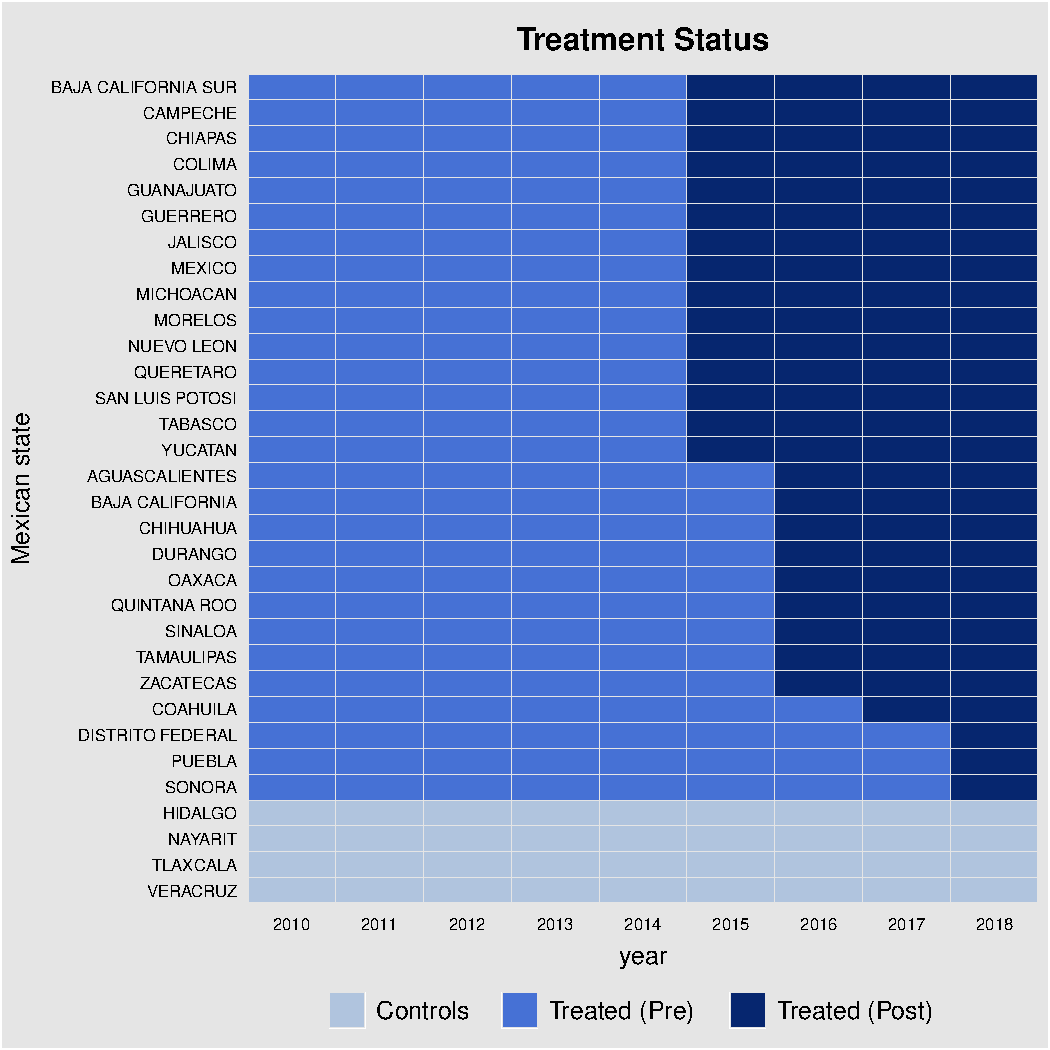
\includegraphics[width=0.75\textwidth]{Figures/reform_treatmentstatus.pdf}     
\captionsetup{justification=centering} 
\end{figure}   
 
\section{Data \label{sec:data}}  

To test the effect of the 2014 Term Limit Reform on public security provision and violence, I build a database on violence and effort placed by federal and municipal-level security forces for all municipalities in Mexico from 2010 to 2018.\footnote{Mexico has 2,467 municipalities. Thus, the total possible number of observation is 22,203 municipality-years (2,467 municipalities X 9 years).} The main outcome of interest is violence proxied by homicide related deaths collected by the National Institute of Statistics and Geography (INEGI for its acronym in Spanish). INEGI reports two homicide data. One the one hand, homicide related deaths that come from the total death certificates marked as ``presumed homicides''. On the other hand, homicide statistics made up of the number of previous investigations initiated for the crime of homicide, by year and state. As noted by \citet{rivera_2012} these datasets do not coincide for a simple reason: the former counts bodies, the latter counts cases. I choose homicides based on death certificates since those based on initiated investigations tend to miscalculate the total number of deaths.\footnote{For instance, borrowing a practical example by \citet{rivera_2012}, consider a mass grave with charred human remains. A preliminary investigation will count the number of deaths, and this will become part of the homicide related deaths figure. However, the investigation will only file one case, regardless of the number of victims found. I thus prefer to count victims rather than cases.} I measure homicides per capita to rule out municipality population differences. Population estimates come from the 2010 Census, the 2015 Population Count (both by INEGI), and CONAPO's population projections at the municipal level. Homicides per capita are highly skewed, with a long right tail of municipalities with substantially greater homicides than others. I therefore run the estimation on the impact of the reform on homicides per capita on logged values. For robustness, following \citet{mackinnon_maggie_1990}, I use the inverse hyperbolic sine (IHS) to transform the main outcome. For robustness, I run estimates based on a second homicide database build by the SNSP.\footnote{For more detail on the SNSP homicide database please see Appendix \ref{appendix:SNSP_homicides}.}



To approximate the level of effort placed by the military I build a novel database on narcotics, arms and laboratories eradicated by the military -army and marines- from 2006 to 2019 at the municipal level  based on information petitions through the Mexican portal INFOMEX.\footnote{Information petitions number 0000700274419 and 0000700274519.} The dataset includes narcotic eradication (kg) of marijuana, heroine, methamphetamine, and cocaine, as well as marijuana and poppy kg per hectare erradicated, eradicated laboratories, and secured cartridges, vehicles, planes, short and long weapons as well as the detection of clandestine airstrips. %I aggregate the data to the yearly level by municipality. 
Another information petition to INFOMEX was made for municipalities to report the number of criminal detentions made month by month to proxy local level police effort. Detentions were aggregated at the yearly and municipal level. As with homicides, detentions and narcotic eradication and laboratories detected are highly skewed. I transform detentions to per capita logged values (also IHS), and narcotic and laboratories using logged (IHS) values as well. 

I follow \citet{klasnja_titiunik_2017} to construct  a proxy for party-level incumbency advantage. %As in the case of Brazil noted by \citet{klasnja_titiunik_2017}, in Mexico mayors face a two-term limit. Parties in Mexico, however, are not subject to term-limits which allows to evaluate party level consequences for term limited candidates. 
I construct two measures to proxy party incumbency advantage. First, an indicator that takes the value of 1 if the party won office in the election at $t+1$ and was an incumbent on $t-1$, 0 otherwise. This analysis identifies the party that wins at $t-1$ and studies the effect of this party barely winning (or losing) at $t$ on outcomes at election $t+1$ following \citet{klasnja_titiunik_2017}. This measure requires at least three rounds of elections, and thus I consider all municipal level elections since 2010 to 2018.\footnote{Municipal electoral calendars vary by state. However, almost all municipalities have three year terms with the exception of some municipalities with non-aligned electoral calendars with State-level ones, or other political circumstances.} A second measure is an indicator that takes the value of 1 if the party won office in the election at $t+1$ and was an incumbent on $t$, 0 otherwise. Different from the Brazilian case discussed by \citet{klasnja_titiunik_2017} where parties do not contest in every election and thus need to adjust estimates unconditional on parties running,\footnote{\citet{klasnja_titiunik_2017} called this outcome ``unconditional victor on running" and measures if a party won at $t+1$ regardless of whether they had a candidate at that time period or not.} in Mexico the three main parties in this time period (PRI, PAN and PRD) always run in elections they have already participated in the past. Thus, there is no bias to be concerned of related to a party's decision to run at $t+1$ given anticipation of their performance at that same time period.  

Lastly, electoral data for recent Mexican elections at the governor and municipal level as well as data on the rollout of the electoral reform at the municipal level comes from \citet{magar_2012} and \citet{magar_2017}. The data compiled from multiple sources including state electoral institutes, Banamex Electoral Database, Voz y Voto, etc. contains voting counts per party as well as candidate lists at the governor level. I construct winning margins at the municipal and state level as the difference between the first and second runner. To measure the number of political parties by municipality, I use the Laakso-Taagepera effective number of parties index.\footnote{\citet{laakso_1979} computes the effective number of parties as the inverse of a Herfindhal-Hirschman Index using party vote shares.} Indicators to measure party-alignment between the Federal executive, state and municipal governors are also build. Appendix Table \ref{tab:descriptive} presents descriptive statistics of the variables used in the paper.

%Lastly, pre-reform municipal level covariates including area, come from INEGI and the Municipal... .

\section{Research Design: Cohort weighted even-study design \label{sec:design}}  
     
Recent literature has shown that in the presence of staggered treatment timing and heterogeneous treatment effects across cohorts, the coefficient from two-way fixed effects models are not causally interpretable \citep{goodman_bacon_2018, callaway_santana_2019, strezhnev_2018, chaisemarting_etal_2019}. Furthermore, for event-study designs \citet{abraham_sun_2020} find that even under strong parallel trends assumption, pre-reform coefficients may not be non-zero and the post-reform coefficients may not correspond with a convex weighted averages of cohort-specific treatment effects at particular lags and leads. In other words, coefficients of a given lag or lead can be biased by the effects from other time periods, and pretrends may be driven by treatment effect heterogeneity.  
  
 To account for potential cohort treatment heterogeneity, I estimate    a cohort weighted event-study design following \citet{abraham_sun_2020} that exploits the staggered implementation of the reform and state-level variation. I saturate the time and unit fixed effects structure so that treated units do not enter the test window as control units. Specifically, I replace the binary indicator variable for the start of the treatment reform with a series of lead/lag indicators $\gamma_k$ for being ``k" years away from treatment. I focus on the window from 8 years prior to treatment to three years afterwards i.e. for $k \in \{-8,3\} $ which correspond to the time period of 2010 to 2018, with 2015 the first year of Term Limit Reform implementation.\footnote{See Figure \ref{fig:treatment_status} where those treated in 2018 have 8 lags prior to treatment, while those treated in 2015 have 3 leads, the full window of analysis for $k \in \{-8,3\} $.} %In addition to including $\gamma_k$ for $k \in \{-8,3\} $, I saturate the model with indicators for years less than 3 years before treatment, and more than three years after treatment. 
I exclude the indicator on $\gamma_{-1}$ to avoid collinearity and for comparison: estimated coefficients are interpreted as the difference relative to $t-1$, i.e. one year prior to the implementation of the electoral reform. Following   \citet{abraham_sun_2020}, I also exclude $k=-8$ due to collinearity. The estimated equation is as follows:

\begin{comment}
\section{Naive Research Design}

 The estimating equation is as follows:
 
\begin{equation}
\label{eq:event_study} 
	y_{mt}=\mu_m + \mu_t  + \sum\limits^{3}_{k=-8, k \neq -1} \gamma_k R_{m} \mathbbm{1}(t-I_{m}=k)  + \sum\limits^{3}_{k=-8, k \neq -1} \Theta'X_{it} \mathbbm{1}(t-I_{m}=k) + \epsilon_{mt}
	%y_{it}=\mu_i + \mu_t  + \sum^3_{-8} \gamma_k + \sum^3_{-8} \Theta'X_{it} \mathbbm{1}(t- + \epsilon_{it}
 xcv\end{equation}
 
 where $\mu_i$ and $\mu_t$ are municipality and year fixed effects, respectively, $\gamma_k$ are the relevant time period indicators, and $X_{it}$ is a matrix of state level covariates interacted with a set of event-year fixed effects $(t-I_{m}=k)$ equal to one when the observation year is $k=-8,-7,...,-2,0,...,3$ years from $I_{m}$ the first year a municipality $m$ implemented reelection. $R_{m}$ is an indicator that takes the value of 1 if municipality $m$ implemented reelection, 0 otherwise; this is interacted with the event-year fixed effects. Conditional on municipal and period fixed effects, $\gamma_k$ represent the annual difference in mean logged homicides per capita between municipalities that implemented reelection relative to those that did not, $k$ years before a municipality implemented reelection. Throughout specifications, standard errors are clustered at the state-level as that is the treatment level.   

Besides pretrends, identification in this setting implies that the staggered roll-out of the electoral reform is orthogonal to municipal-specific characteristics, conditional on municipal and year fixed effects. In other words, this implies as-if random assignment to the treatment status visualized in Figure \ref{fig:treatment_status}. If say, strong governors delay or adjust the implementation of the reform according to their political agenda or calendar, then identification would fail. To address this problem equation \ref{eq:event_study} interacts the state-level covariates with the linear time trend to adjust for any changes correlated to the evolution of governors strength, the term $X_{it} \mathbbm{1}(t-I_{m}=k)$. Covariates include governor winning margin and an indicator of governor party alignment with the Federal Executive, since pressure from former President Enrique Peña Nieto modified state legislators approval of the electoral reform, particularly for PRI states. Identification assumption implies now that conditional on municipal and year fixed effects, and linear trends in state-level covariates, unobserved factors are not correlated with the electoral reform treatment assignment over time.\footnote{I'm in the process of adding municipal level covariates as well.} 
   
 Figure \ref{fig:event_study_wcovariates} presents the event-study estimates. The term-limit reform increased the number of homicides per capita since the first year of implementation onwards. Related to the pre-trend identification assumption, while there is some evidence that the trend is increasing homicides from period $t-5$ to $t-3$ this trend decreases two periods prior to treatment $t$. Thus, little evidence of pre-trends exist in the data.\footnote{Appendix Table \ref{tab:abraham_sun_transformations} shows the estimates of equation \ref{eq:event_study} considering various main outcome transformations, with no transformations in columns (1) and (2), normalizing estimates by population rates in column (3) and (4), and logged values of per capita homicides in column (5) and (6). Overall, we find evidence of pretrends and positive effects of the electoral reform on violence across specifications, albeit noisy when we do not consider population adjustments and logged values. These results suggest the need to rule out outlier observations and increase comparability across municipalities by considering population differences.} %To further probe results, the following analyses will attempt to tease out bias related to (a) potential violation of the parallel trend assumption, or (b) differential treatment effect across units and across time which might bias results. 
 
 %Further, note in Figure \ref{fig:event_study_did} that we violate the constant treatment effects assumption. As noted by \citet{goodman_bacon_2018} and \citet{strezhnev_2018}, even with no pre-trends, if there is heterogeneous treatment effects across units or time, two-way fixed effects (TWFEs) estimates are biased. We can see this if we estimate a TWFE model, which -not surprisingly- shows a negative effect of the electoral reform on homicides per capita. What explains such sign flip relative to the \emph{positive} ``event-study'' DiD estimate found in Figure \ref{fig:event_study_wcovariates}? The aforementioned violation of constant treatment effects across units and time. As noted by \citet{goodman_bacon_2018}, the decomposition of the probability limit of the TWFE DiD estimator is equal to the ``variance-weighted average treatment effect on the treated'' (VWATT) plus the ``variance weighted common trends'' (VWCT) (a generalized parallel trend with timing variation,\footnote{Captures the notion that different groups might not have the same underlying trend in outcome dynamics pre treatment, and could bias the DiD estimate} which equals zero, if such assumption holds) \emph{minus} the ``weighted sum of the change in treatment effects'' ($\Delta$ATT) or the difference between treatment units after treatment and control units after treatment. If positive and sizable, this last term can potentially flip the sign observed by the VWATT. I find this to be the case, and as such present an important source of bias in the TWFE estimation. 
 

 
\begin{figure}[h] 
\centering
\caption{Effect of Electoral Reform of 2014 on Homicides} 
\label{fig:event_study_wcovariates}

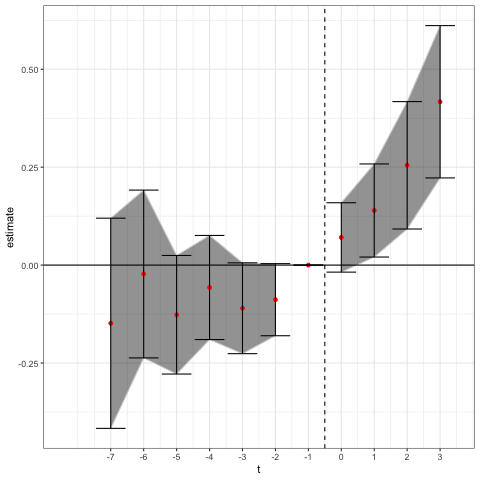
\includegraphics[width=0.8\textwidth]{Figures/event_study_wcovariates}
       \captionsetup{justification=centering} 

\bigskip
{\textbf Note: Estimates conditional on state-level covariates interacted with linear time trend. 95\% confidence intervals reported.}
\end{figure}    
 
 \subsection{Main Results and Identification}
 
  \end{comment}
  

 

 %Event-study designs rely on three identifying assumptions: (1) generalized form of parallel trends, (2) no anticipation of the treatment, and (3) no variation across cohorts. Furthermore,
 %As noted by \citet{abraham_sun_2020}, besides no pretrends, event study designs rely on the identifying assumption of no anticipation of treatment and treatment effect homogeneity across treated groups, i.e. that cohorts share the same path of treatment effect. After controlling for covariates (and covariates interacted by event-year fixed effects), cohorts may still vary if states selected their treatment timing based on treatment effects.\footnote{Note that no pretends is till compatible with cohort treatment heterogeneity, since parallel trends prior to treatment ``only rule out selection in the initial treatment timing based on the evolution of the baseline outcome" \citep{abraham_sun_2020}.} If pretrends and no anticipation of treatment hold (as is our case and will be shown later) but there is heterogeneous effects across cohorts, then non-zero pre-reform estimates for municipalities showed in Figure \ref{fig:event_study_wcovariates} are not evidence of pretends \citep{abraham_sun_2020}. In other words, heterogeneous effects across cohorts would imply spurious pretrends when actually none exist. 
 
 
 \begin{equation}
\label{eq:abraham} 
y_{mt}=\mu_m + \mu_t + \sum^{5}_{e=1} \sum^3_{k=-7, \neq {-8,-1}} \gamma_{e,k}(1\{E_i=e\} \cdot R^k_{m,t}) + \sum^{5}_{e=1} \sum^3_{k=-7, \neq {-8,-1}}  \Theta'X_{s(m)t} (1\{E_i=e\} \cdot R^k_{m,t}) + \epsilon_{mt}
%y_{mt}=\mu_m + \mu_t + \sum^5_{e=1} \sum^{3}_{k \neq {-8,-1}} \gamma_{e,k}(1\{E_i=e\} \cdot R^k_{m,t}) + \sum^5_{e=1} \sum^{3}_{k \neq {-8,-1}}  \Theta'X_{m(s)t} (1\{E_i=e\} \cdot R^k_{m,t}) + \epsilon_{mt}
%y_{mt}=\mu_m + \mu_t + \sum^5_{e=1} \sum^{3}_{k \neq {-1,-8}} \gamma_{e,k}(1\{E_i=e\} \mathbbm{1} (t-I_{m}=k)  ) + \sum\limits^{3}_{k=-8, k \neq -1} \Theta'X_{it} \mathbbm{1}(t-I_{m}=k) + \epsilon_{mt}
%y_{mt}=\mu_i + \mu_t + \sum^5_{e=1} \sum^{3}_{k \neq {-1,-8}} \gamma_{e,k}(1\{E_i=e\}\cdot R^k_{m,t} ) + \sum\limits^{3}_{k=-8, k \neq -1} \Theta'X_{it} \mathbbm{1}(t-I_{m}=k) + \epsilon_{mt}
\end{equation} 
  
where $E_i$ are cohort-specific indicators if a Mexican state removed term limits in a given year.\footnote{As noted in Figure \ref{fig:treatment_status}, there are five treatment cohorts including the never treated. The never-treated cohort is made up of the municipalities in the states of Hidalgo, Nayarit, Tlaxcala and Veracruz.} $R^k_{m,t}\in \{0,1\}$  is the Term Limit Reform treatment status indicator at period $k$ relative to treatment, for municipality $m$ at calendar time $t$.\footnote{$t=e+k$.} $X_{s(m)t}$ is a matrix of state $s$ (municipal $m$) level covariates interacted with the set of cohort-specific fixed effects including pre-treatment governor elections winning margin and governor partisanship with central government.  The year indicators by treatment cohort  $\gamma_{e,k}$ are the difference-in-difference (DiD) estimators for the Cohort Average Treatment Effects (CATTs). Conditional on municipal and period fixed effects, as well state-level covariates, these CATTs represent the annual difference in mean logged homicides per capita between municipalities that removed term-limits relative to those that did not, $k$ years before and after treatment. Standard errors are clustered at the state-level as that is the treatment level of the Term Limit Reform.    

I take the linear combination of the CATTs for each relative time period $k$, weighting each cohort by its relative share of the sample, to construct the interaction weighted (IW) estimator of \citet{abraham_sun_2020}:   

\begin{equation}
\hat{\nu}_g=\frac{1}{|g|}\sum_{k \in g}\sum_e \hat{\gamma_{e,k}} \hat{Pr}\{E_i=e | E_i \in [-k, T-k]\}	
\end{equation}

where $\hat{\gamma_{e,k}}$ is returned from equation \ref{eq:abraham} and $\hat{Pr}\{E_i=e | E_i \in [-k, T-k]\}$  are the estimated weights equal to the share of each cohort in the relevant time period, normalized by the size of  $g$, with $g$ the universe of the $k$ periods relative to treatment. Since I estimate a IW estimator per year $|g|=1$.


\subsection{Main Results \label{sec:main_results}}

\begin{figure}[h] 
\begin{center}
	
\caption{Effect of Term Limit Reform of 2014 on Violence \\ -log transformation, 95\% confidence intervals-}
\label{fig:event_study_log}

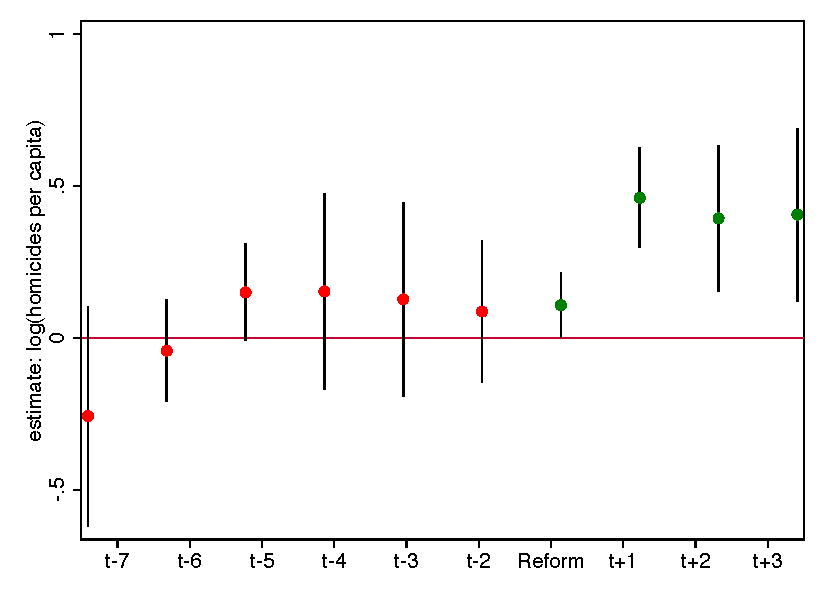
\includegraphics[width=1\textwidth]{Figures/event_study_log.pdf}
       \captionsetup{justification=centering}
\end{center}
 Note: Figure \ref{fig:event_study_log} shows the IW estimators following \citet{abraham_sun_2020} for each lead and lag relative to the first year a municipality implemented reelection. These estimates correspond to those of Table \ref{tab:abraham_sun_lagdv} column (1). Red points show pre-treatment estimates, while green ones are post-treatment. 
 
\end{figure}   
       
 

\begin{table}[htbp]\def\sym#1{\ifmmode^{#1}\else\(^{#1}\)\fi}
\centering
\caption{Effect of 2014 Term Limit Reform on Violence}
\label{tab:abraham_sun_lagdv}
\scalebox{1}{
\begin{tabular}{lcc}
\hline \hline
\\ \multicolumn{3}{l}{Dependent variable:}\\
& \multicolumn{1}{c}{log(homicide per capita)} & \multicolumn{1}{c}{log(homicide per capita)$^{a}$} \\
& \multicolumn{1}{c}{(1)} & \multicolumn{1}{c}{(2)} \\
\cmidrule(lrr){2-2}  \cmidrule(lrr){3-3}\\
\addlinespace
Lag 7 years &      $ 0.0360^{} $ &  $ 0.2352^{} $   \\
& ($ 0.0653$) & ($ 0.3443 $) \\
Lag 6 years &          $ 0.3874^{*} $ &   $ -0.0161^{} $  \\
& ($ 0.2212$) & ($ 0.1898 $) \\
Lag 5 years &        $ 0.3205^{} $ &   $ 1.5038^{***} $ \\
& ($ 0.1991$) & ($ 0.2806 $) \\
Lag 4 years &         $ 0.3264^{*} $ &      $ 1.5281^{***} $  \\
& ($ 0.1734$) & ($ 0.2335 $) \\
Lag 3 years &        $ 0.3200^{*} $ &     $ 1.8256^{***} $ \\
& ($ 0.1610$) & ($ 0.2652 $) \\
Lag 2 years &        $ 0.1083^{} $ &    $ 1.4292^{***} $  \\
& ($ 0.0901$) & ($ 0.2652 $) \\
Reform, time 0 &        $ 0.0420^{} $ &     $ -0.2415^{***} $ \\
& ($ 0.0264$) & ($ 0.0701 $) \\
Lead 1 year &         $ 0.1309^{**} $ &       $ 0.6128^{***} $ \\
& ($ 0.0529$) & ($ 0.1012 $) \\
Lead 2 years &         $ 0.3410^{***} $ &      $ 0.4352^{***} $  \\
& ($ 0.1162$) & ($ 0.0885 $) \\
Lead 3 years &        $ 0.4996^{**} $ &     $ -0.4281^{} $ \\
& ($ 0.2362$) & ($ 0.2647 $) \\
\addlinespace
Observations       &                 14,587        &          14,587  \\
R-squared        &              0.7157        &           0.8202   \\
Mun. FEs       &     \checkmark         &  \checkmark    \\
Year. FEs       &     \checkmark         &  \checkmark   \\
Controls$^b$   &          &   \checkmark     \\
Cohort weighted   &   \checkmark       &   \checkmark    \\
\hline \hline
\multicolumn{3}{p{0.8\textwidth}}{\footnotesize{Notes: Coefficients show IW estimators following \citet{abraham_sun_2020}. Two relative time periods (lag 8 and 1) are removed to avoid collinearity problems noted by \citet{abraham_sun_2020}. Standard errors in parentheses are clustered at the state level, with the following significance-level: $^{***}$ 1\%; $^{**}$ 5\%; and $^*$ 10\%, that refer to two-sided t-test with the null hypothesis equal to 0 for each relative time period. $^a$ Refers to the inverse hyperbolic sine transformation. $^b$ State-level controls include governor winning margin in last pre-treatment election and an indicator of whether the governor's party is the same as the federal incumbent party.}} \\
\end{tabular}
}
\end{table}
  

Table \ref{tab:abraham_sun_lagdv} reports the IW estimator\footnote{From here on all tables report IW estimators.} for each lead and lag relative to the first year a municipality implemented reelection.\footnote{Appendix Table \ref{tab:abraham_sun_transformations} compares cohort weighted vs non weighted IW estimators. There are no pretrends when we do not adjust for cohort weights. Non-weighted estimates should be interpreted with caution as noted by \citet{abraham_sun_2020}.} The first column reports logged values while the second shows IHS transformations. All specifications control for pre-treatment state characteristics  interacted with cohort-specific fixed effects, as well as municipal and year fixed effects. Dynamic time trends disappear when we account for violence trends when we include the lag of the outcome (see Appendix Table \ref{tab:abraham_sun_transformations} column 6).\footnote{Including a lag outcome may introduce Nickell bias. More importantly, the lagged outcome conflates controls for heterogeneity and modeling dynamic treatment effects. To avoid these problems I only control for pretreatment outcomes to deal with heterogeneity. Alternatively, I use matching on pre-treatment outcomes and find that results show similar effects. Moreover, if I remove the lagged outcome it does not affect results and shows the existence of dynamic time trends. These results are available upon request.}  

Column (1) shows that the reform increased homicides per capita in 10.8\% the first year of implementation, with an increase to 46.16\% one year after implementation (for a visual representation see Figure \ref{fig:event_study_log}). This effect remains relatively constant two and three years after implementation. Not only are results robust to the IHS transformation but higher that logged specifications as noted in column (2). Importantly, since we control for the lag of (logged or IHS) homicides per capita, we rule out effect is driven by violence time trends.  

%Here report a time-corrected Wald ratio (WALD-TC) as well as a changes-in-changes Wald ratio (WALD-CIC) following Chaisemartin (2017) fuzzy DiD design (Ali's suggestion).  

\subsection{Identification \label{sec:identification}}
 
Once we consider cohort weights, I find strong evidence of parallel trends using the logged and IHS transformation as noted in Appendix Table \ref{tab:abraham_sun_noweights} columns (2) and (4), respectively. As noted in columns (1) and (3) if cohort weights are not considered pretrends are found. These estimates, however, are considered biased since leads and lags are contaminated by the effects from other periods \citep{abraham_sun_2020}. 
 
Besides pretrends, identification in this setting implies that the staggered roll-out of the Term Limit Reform is orthogonal to municipal-specific characteristics, conditional on municipal and year fixed effects. This implies {\emph as-if} random assignment to the treatment status visualized in Figure \ref{fig:treatment_status}. If say, strong governors delay or adjust the implementation of the reform according to their political agenda or calendar, then identification would fail. To address this problem equation \ref{eq:abraham} interacts the state covariates with cohort-specific fixed effects to adjust for any changes correlated to the evolution of governors strength, the term $X_{s(m)t} (1\{E_i=e\} \cdot R^k_{m,t})$. Covariates include governor winning margin and an indicator of governor party alignment with the Federal Executive, since pressure from former President Enrique Pena Nieto modified state legislators approval of the electoral reform, particularly for PRI states (for more detail see Section \ref{sec:reform}). Identification assumption implies now that conditional on municipal and year fixed effects, and cohort specific linear trends in state-level covariates, unobserved factors are not correlated with the electoral reform treatment assignment over time.%\footnote{I'm in the process of adding municipal level covariates as well.}   
 

%First, if state-covariates are taken into account there is mean difference prior to treatment between treated and control municipalities. In other words, if we do not consider the involvement of governors in the implementation period of the electoral reform across states, state level characteristics are correlated with treatment assignment. This is to be expected as governors in control of state legislators determined the term-limit removal implementation time period as discussed in Section \ref{sec:reform}. Second, if we do not consider heterogeneous treatment effects, we might find spurious evidence of no pretrends: Appendix Table \ref{tab:event_study_noweights} shows non-cohort weighted estimates, with and without controlling for state-level differences across lags and leads and cohorts. Pretrends seem present across specifications. However, given variation in treatment timing across units, the coefficients of leads and lags are contaminated by the effects from other periods, arising apparent -but non-existent- pretrends \citep{abrahams_sun_2020}. That is why estimates from  Appendix Table \ref{tab:abraham_sun_noweights} columns (1) and (3) are considered biased. 
 

An additional identification assumption in event-study designs speaks to no anticipatory behavior from municipalities (or states) to the implementation of reelection. If states have private knowledge of the future treatment path this may change their behavior in anticipation to being treated and thus the potential outcome prior to treatment may not be that of baseline outcomes: estimated coefficients may reflect the anticipatory effects of the reform rather than differences in untreated potential outcomes between untreated and treated groups. %\citep{malani_rief_2015}.
In this setting, knowledge from incumbents of the term limit removal could lead to a decrease in public security (and public good) provision since this will be the period a term limited politician could extract rents or pursue clientelistic practices without the electoral penalty of reelection. The violation of this identification assumption would lead to a (positive) bias of concern. To see if this assumption holds I test whether early vs late adopters differed in their estimated effects. As seen in Appendix Figure \ref{fig:CDLZ}, this is not the case: there is wide variation in estimated coefficients across early (red) and late (blue) adopters of the reform, conditional and unconditional on state covariates.\footnote{For more detail on how I compare early to late adopters, please see Appendix \ref{appendix:CDLZ}.}


In short, taking together pretrends, evidence on no-anticipatory behavior from municipalities (states) and cohort weighted estimates that account for treatment effect heterogeneity, I find a robust and unbiased positive effect of reelection in homicides per capita.  The following section further probes the results through different robustness and falsification tests.%Other way to test this assumption is the no het effects of governor alignment with executive. 

\subsection{Robustness and Falsification tests, and Sensitivity Analysis \label{sec:robustness}}  
   
I run several robustness checks to confirm main findings. %Appendix Table \ref{tab:abraham_sun_lagdv} shows that results are robust (and actually stronger both in magnitude and significance) when we control for the lag of the outcome variable to account for time trends. Using logged values, we see an increase in homicides per capita from 23.4 to 40.6\% when take into account trends, while with the IHS transformation homicides per capita increase from 27.4 to 55.6\%. Importantly, short-term increasing dynamic trends disappear once we consider lagged violence. This suggests that there were important pre-treatment differential violence.
To rule out concerns regarding dataset selection, Appendix Table \ref{tab:abraham_sun_lagdv_voutcomes} compares the effect of the Term Limit Reform on logged homicides per capita from different sources, INEGI, and the old and new methodology of homicides based on criminal cases from the SNSP. All specifications show parallel trends, especially 4 years prior to treatment. Moreover, all show positive and significant effects (mostly to the 1\% level). If I combine through averaging homicide data from SNSP's old and new methodology there is evidence of pretrends four years prior to treatment, and strong positive and stable effects of the term limit reform on homicides per capita.\footnote{There is no agreement if data captured through the new methodology can be paired with the old one due to differences in the filing of criminal cases. Estimates of column (4) should be interpreted with caution.} Results remain unchanged if we consider IHS transformations instead of logged values. 

Two additional tests are done to increase the robustness of results. First, I check if results hold even with possible violations of parallel trends exist. As described in Appendix \ref{appendix:sensitivity}, results are robust even if we relax the parallel trend assumption to account for linear violations following \citet{rambachan_roth_2019}. 
  
%I run three additional robustness checks to asses the validity of main results and specially of the existence of pretrends. Appendix Figure \ref{fig:non_did} plots two non-difference-in-difference methods to test the electoral reform treatment effect on violence on panel data conceptually similar to DiD estimates. Panel A plots the results of estimating the generalized synthetic control method following \citet{xu_2017} while Panel B presents the matrix completion method following \citet{athey_etal_2020}. Two observations. First, both methods show strong pretrend evidence. Second, while there seems to be a short term negative treatment effect, followed by a potential reversal, the number of states with various post-treatment years is relatively small, creating large confidence intervals. Nonetheless, results seem to convey the general effect identified in the event-study design, a positive trend across time from $t+2$ onwards on homicides per capita due to reelection, as well as pretrends. 
 
   
I conduct a final analysis to validate main results. I perform a falsification test that checks whether the results are being driven by other mechanism that is not the electoral reform staggered rollout. I run 1,000 simulations following equation \ref{eq:abraham} and the specification of Table \ref{tab:abraham_sun_lagdv} column (1). This specification is the most robust specification that includes state covariates interacted with cohort-specific fixed effects, the lag of the main outcome to account for time trends, and municipal and year fixed effects. IW estimators are shown using cohort weights. In each simulation, I randomly assign each Mexican state to treatment and control using a random Bernoulli draw, keeping the proportion of treated units per year (e.g. there are 15 treated states out of 32 in the first treatment year (2015); this proportion is kept when assigning treatment randomly for the first year of treatment). In other words, I keep the same cohort size distribution of states. Thus, I randomly assign treatment following the observed treatment incidence. I then re-estimate the parameter of interest in each placebo simulation using the full sample of municipalities of Table \ref{tab:abraham_sun_lagdv}. Appendix Figure \ref{fig:falsification} shows the resulting distribution of the 1,000 estimated beta coefficients (cohort weighted) for each lag and lead (IW estimates). The average estimated effect of the placebo is very close to zero (red dashed line), and its highly statistically unlikely that the estimates of Table \ref{tab:abraham_sun_lagdv} column (1) (blue line) could have been drawn from such a distribution. 

If term limit removal strengthened voter accountability, what explains these paradoxical results? The following section delves into the mechanisms, specifically the role of electoral incentives on incumbents and the party on hold of the central government. Section \ref{sec:alternative_mechanism} proceeds by ruling out alternative potential mechanisms, including adverse candidate selection (Section \ref{sec:adverse_selection}), citizens public security demands (Section \ref{sec:alternative_voter_demand}) and state capture by criminal organizations (Section \ref{sec:alternative_capture}).

\section{Mechanisms: Reelection Reform and Incumbency Advantage \label{sec:mechanism}}

%\subsection{Reelection Reform and Incumbency Advantage}    
 
If reelection strengthen voter accountability, what explains this paradoxical result of increasing violence? As discussed in Section \ref{sec:theory}, incumbent politicians are accountable to both political parties and voters. Policy preference misalignment from both principals, however, may yield inefficient public good provision. While it may be clear that voters prefer criminal deterrence and a reduction in violence,\footnote{It may not be as evident that voters prefer more public security provision given the externalities that the War on Drugs may create. This is further discussed in Section \ref{sec:alternative_voter_demand}.} preferences of incumbent parties is not evident in this setting. the behavior of parties, however, depends on electoral incentives. As noted in Section \ref{sec:theory} if providing public security is costly, politicians may prefer to forbear the provision of public security. 

To test this mechanism I run %a %regression discontinuity design (RDD) of close elections as well as 
a difference-in-discontinuity design that exploits the staggered rollout of the electoral reform and compares only municipalities with close elections.%\footnote{I focus on close elections to rule out the potential omitted variable bias from party and candidate level characteristics and other idiosyncratic factors that may affect the incumbency advantage. While \citet{eggers_2017} shows that even in close election designs we cannot rule out quality-based incumbency advantage results, in Section \ref{sec:adverse_selection} I rule this specific mechanism out.}
 Specifically, I assess if the electoral reform led to an incumbency advantage that could trigger a decrease in the provision of public security and a subsequent increase in violence due to the vacuum of power left for grabs to DTOs.\footnote{I also run a regression discontinuity design of close elections, splitting the sample before and after the treatment of the reform. These results need to be considered as naive and biased since we would need to assume that that the value of incumbency in term limited and non-term limited cases is the same. \citet{fowler_hall_2014} make such quasi-parallel trend assumption but I prefer to actually test it using an difference-in-discontinuity in close elections design. The results of this exercise can be found in Appendix \ref{appendix:rdd}.}   
  

\subsubsection{Difference-in-Discontinuity of close elections design}  
      
Following \citet{grembi_2016} and \citet{gelman_imbens2014}, I fit a local linear regression for municipalities within an Imbens-Kalyanaraman optimal bandwidth distance $h$ to the cutoff (=0), using as forcing variable the winning margin of executive local elections.\footnote{A rectangular kernel would give the same results as taking $E[Y]$ at a given bin on the distance to the cutting threshold. Other types of kernels, such as a triangular kernel, gives more weight to observations closer to the cutoff. I choose the latter for all estimations presented while estimations using a rectangular kernel are available upon request. Results are almost unchanged using the latter.} In other words, I compare only municipalities in close elections and thus restrict the sample to those within a certain distance $h$ to the threshold, i.e. $D_{mt} \in [D_b-h, D_b+h]$ for municipality $m$ in time period $t$. By comparing municipalities where a party barely wins an election to municipalities where a party barely loses, the design allows to isolate the causal effect of winning office from the spurious correlation between current and future electoral success.\footnote{For example, potential correlation that could arise, noted by \citet{klasnja_titiunik_2017}, is that parties with good reputation or strong candidates are more likely to succeed in an electoral contest.} Furthermore, the difference-in-difference setup allows to tease out any time-variant and time variant confounding variation as long as parallel trends and no anticipatory behavior from municipalities (states) holds. Lastly, following \citet{abraham_sun_2020} I present IW estimators to account for potential treatment effect heterogeneity. Given the discontinuity implicit setup, the results are local by construction. 

The specification of the event-in-discontinuity in close elections design is the following:

\begin{equation}
\begin{split}
y_{mt}=\mu_m + \mu_t + \sum^5_{e=1} \sum^0_{k=-5, \neq {-6,-1}} \gamma_{e,k}(1\{E_i=e\} \cdot R^k_{m,t}) + \sum^5_{e=1} \sum^0_{k=-7, \neq {-5,-1}}  \Theta'X_{it} (\mathbbm{1}(E_i=e)\cdot R^k_{m,t})  \\
+ f_{(.)}(margin)_{mt} + \sum^5_{e=1} \sum^0_{k=-5, \neq {-6,-1}} \nu_{e,k}(1\{E_i=e\} \cdot R^k_{m,t} \cdot  f_{(.)}(margin)_{mt} )+ \epsilon_{mt}
\end{split}
\end{equation}     

where $f_{(.)}(margin)_{mt}$ is the RD polynomial on winning margin for municipal election $m$ at calendar time $t$, having $f_{(.)}$ take various polynomial approximations from quadratic to quartic. $\sum^5_{e=1} \sum^{0}_{k=-5, \neq {-6,-1}} \nu_{e,k}(1\{E_i=e\} \cdot R^k_{m,t} \cdot  f_{(.)}(margin)_{mt} ) $ is the RD polynomial interacting the $E_i$ cohort-specific indicators and the electoral reform treatment indicator. Given that municipal elections occur every three years at maximum, and the reform was enacted in 2014 and all municipalities in the study period had only one election, there are no leads. Thus $k$ relative time periods run from  $k \in\{-6,-5,...,0\}$. As with equation \ref{eq:abraham}, to avoid collinearity I exclude two time period indicators, in this case that of $k=-1$ and $-6$.  Period $k=-2$ does not exist since there are no municipal elections two periods prior to the implementation of the electoral reform. As before, the period indicators by treatment cohort  $\gamma_{e,k}$ are the DiD estimators for the Cohort Average Treatment Effects (CATTs). I take the linear combination of the CATTs and the relative cohort weights to construct the IW estimator. Standard errors are clustered at the state level as that is the level of treatment. 
 
 \begin{table}[htbp]\def\sym#1{\ifmmode^{#1}\else\(^{#1}\)\fi}
\centering
\caption{Event-in-Discontinuity in close elections model: Effect of 2014 Term Limit Reform on Incumbency Advantage}
\label{tab:incumbency_wpolynomials}
\scalebox{0.8}{
\begin{tabular}{lcc}
\hline \hline
\\ \multicolumn{3}{l}{Dependent variable:}\\
& \multicolumn{1}{c}{Incumbent at t-1 won at t+1}  & \multicolumn{1}{c}{Incumbent at t won at t+1} \\
& \multicolumn{1}{c}{(indicator)}  & \multicolumn{1}{c}{(indicator)} \\
& \multicolumn{1}{c}{(1)} & \multicolumn{1}{c}{(2)}  \\
\cmidrule(lrr){2-2}  \cmidrule(lrr){3-3} \\
\addlinespace
& \multicolumn{2}{c}{linear polynomial} \\
\cmidrule(lrr){2-3} \\
4 Elections prior &       $ -0.0006^{} $ &       $ 0.0578^{*} $  \\
& ($ 0.0681 $ ) & ($ 0.0320 $ ) \\
3 Elections prior &       $ 0.0747^{} $ &        $ -0.1118^{***} $ \\
& ($ 0.1660 $ ) & ($ 0.0343 $ ) \\
2 Elections prior &          $ 0.1262^{} $ &       $ 0.0773^{} $ \\
& ($ 0.0965 $ ) & ($ 0.1420 $ ) \\
Election after Reform &         $ -0.0025^{} $ &        $ 0.1355^{***} $ \\
& ($     . $ ) & ($     . $ ) \\
Observations          &              2,002     &              3,084 \\
R-squared        &          0.5605   &          0.5887 \\
\\
& \multicolumn{2}{c}{quadratic polynomial} \\
\cmidrule(lrr){2-3} \\
4 Elections prior &       $ -0.1093^{***} $ &       $ 0.0657^{} $  \\
& ($ 0.0144 $ ) & ($ 0.0433 $ ) \\
3 Elections prior &       $ 0.3221^{***} $ &        $ -0.2892^{***} $ \\
& ($ 0.0608 $ ) & ($ 0.0557 $ ) \\
2 Elections prior &          $ 0.0467^{} $ &       $ 0.0358^{} $ \\
& ($ 0.0801 $ ) & ($ 0.1267 $ ) \\
Election after Reform &         $ -0.1600^{***} $ &        $ 0.1111^{***} $ \\
& ($     . $ ) & ($     . $ ) \\
Observations          &              2,766     &              4,038 \\
R-squared        &          0.5478   &          0.4066 \\
\\
Mun. FEs        &     \checkmark         &  \checkmark   \\
Year. FEs     &     \checkmark         &  \checkmark  \\
Controls$^a$  &    \checkmark     &       \checkmark \\
Cohort weighted  &         \checkmark &         \checkmark \\
\hline \hline
\multicolumn{3}{p{0.9\textwidth}}{\footnotesize{Notes: Coefficients show IW estimators following \citet{abraham_sun_2020}. Two relative time periods (lag 6 and 1) are removed to avoid collinearity problems noted by \citet{abraham_sun_2020} or because they are collinear or inexistent, like lag time period 2. Standard errors in parentheses are clustered at the state level for estimates in saturaded model. Significance-level: $^{***}$ 1\%; $^{**}$ 5\%; and $^*$ 10\%, that refer to two-sided t-test with the null hypothesis equal to 0 for each relative time period. $^a$ State-level controls include governor winning margin in last pre-treatment election and an indicator of whether the governor's party is the same as the federal incumbent party. Logged homicides per capita at the municipality level are also included as controls.}} \\
\end{tabular}
}
\end{table}
               
 
Table \ref{tab:incumbency_wpolynomials} presents results. Column (1) shows the effect of the electoral reform on the probability of winning at $t+1$, if it was the incumbent on $t-1$ following \citet{klasnja_titiunik_2017}, while column (2) presents the effect on the probability of winning at $t+1$ if the incumbent won at t. Columns (2) and (4) present IW estimators. As noted, the electoral reform generated an incumbency advantage of 35 percentage points, a result significant to the 10\% level and robust across different polynomial approximations (column 1). Results are stronger if we compare incumbents at $t$ that barely won at $t+1$ relative to those that barely lost: the electoral reform increased the probability of winning in the following election between 53 to 77 percentage points depending on the specification, a result significant to the 1\% level (see column 2). Importantly, as noted by \citet{fowler_hall_2014} we need to divide the observed coefficients and their standard errors by 2 in order to get the actual incumbency advantage. ``The  incumbency advantage is doubled because the winning party has both the benefit of being the incumbent party and the benefit of the other party not having this advantage (p. 512).'' 
       
To validate causal effects three identification assumptions need to hold. First, cohort weighted specifications need to show parallel trends for both incumbency advantage measures. As seen in Table \ref{tab:incumbency_wpolynomials}  this is the case. Cohort weights further assure that parallel trends are not spurious due to correlation between the $k$ period indicators relative to treatment implementation. Second, no anticipatory behavior from municipalities should be found; since we are only taking into account one election cycle post-treatment, we don't anticipate incumbents reacting in such a short time window. %[MISSING]%this is the case when running an ``event-to-event" analysis following \citet{cengiz_etal_2019}: there is no clustering in estimated coefficients on early and late state adopters.\footnote{Results available upon request.} 
Third, the design would be invalid if parties could manipulate close elections and sort themselves to those that imply a higher probability of winning. Two tests are commonly used to show validity on the design: (a) no covariate jump at the discontinuity on relevant pre-treatment variables and (b) density tests to see whether the number of municipalities above (or below) the cutoff threshold is significantly different from the number of municipalities below (or above). Appendix Figure \ref{tab:incumbency_wpolynomials_pop} showes evidence of no significant jump at the discontinuity of municipal population.\footnote{Next iteration of this working paper will include validation on municipal GDP, revenue and expenditures, geographic location and previous victory.} Furthermore, Appendix Figure \ref{fig:mccrary} shows no density difference between municipalities just above and below the cutoff.\footnote{Given the reduction in sample size from Table \ref{tab:abraham_sun_lagdv} to Table \ref{tab:incumbency_wpolynomials} one could have a concern that main results no longer hold in this close election setting. Appendix Table \ref{tab:abraham_sun_local} shows this is not the case by estimating results of Table \ref{tab:abraham_sun_lagdv} using as sample only the municipalities of the sample of Table \ref{tab:incumbency_wpolynomials}.}   

Overall, results show the Term Limit Removal Reform increased incumbent probability of winning at future elections. If this is the case, then we should expect a decrease in the effort placed by security forces in the country, especially from the party in government, the PRI. Federal forces, particularly the military in charge of tackling DTOs, should decrease the amount of narcotic crackdowns and seizures. Furthermore, this should generate a downward effect to local proxies, i.e. mayors in charge of tackling down local crime. In fact, this is what I find. 

\subsection{Electoral Reform and Effort placed by Security Forces} 
   
Table \ref{tab:effort} columns (3) to (8) show IW estimates for the effect of the reform on the eradication of kilograms of heroine and methamphetamine, and laboratories seizures. Odd columns compare those municipalities with at least one activity performed by the military, while even columns include those municipalities with no activity at all. In other words, odd columns show the effect of the Term Limit Reform comparing municipalities with at least one security activity with those with multiple, while even columns present the effect of the reform on municipalities with security activity relative to no activity at all. As observed, the reform decreased the amount of cocaine and methamphetamine eradicated, a result particularly strong three years after the reform was implemented. Cocaine seized kilograms decrease in 2.9\% (a result significant to the 10\% level) if we consider only municipalities that saw some military activity to 1.2\% (significant to the  10\% level) if we consider all municipalities, with and without military intervention. Likewise, methamphetamine decrease in 20.43\%, significant to the 1\% level in municipalities with no military activity and 9.15\%, significant to the 1\% level, considering all municipalities. For the case of laboratories, seizures decreased in 3.8\% (significant to the 10\% level) for municipalities with military intervention and 2.01\% when we include all municipalities (significant to the 5\% level). All results show strong parallel trends.\footnote{Similar decreasing results are found for the eradication of poppy, marijuana, and the seizure of short and long arms, vehicles, clandestine air-paths, grenades and cartridges, but pretrends are found in these cases for all lags.}   

\begin{landscape}
\begin{table}[htbp]\def\sym#1{\ifmmode^{#1}\else\(^{#1}\)\fi}
\centering
\caption{Effect of 2014 Term Limit Reform Security Forces Effort, cohort weighted estimates}
\label{tab:effort}
\scalebox{0.70}{
\begin{tabular}{lcccccccc}
\hline \hline
\\ \multicolumn{9}{l}{Dependent variable:}\\
& \multicolumn{2}{c}{Local Police} & \multicolumn{6}{c}{Military}  \\
\cmidrule(lrr){2-3}  \cmidrule(lrr){4-9} \\
& \multicolumn{2}{c}{log(detained per capita)}  & \multicolumn{2}{c}{heroine, eradicated kg}  & \multicolumn{2}{c}{methamphetamine, eradicated kg} & \multicolumn{2}{c}{laboratories destroyed}  \\
&  & \multicolumn{1}{c}{(relative to none)} &  & \multicolumn{1}{c}{(relative to none)} &  & \multicolumn{1}{c}{(relative to none)} & & \multicolumn{1}{c}{(relative to none)} \\
& \multicolumn{1}{c}{(1)} & \multicolumn{1}{c}{(2)} & \multicolumn{1}{c}{(3)} & \multicolumn{1}{c}{(4)} & \multicolumn{1}{c}{(5)} & \multicolumn{1}{c}{(6)} & \multicolumn{1}{c}{(7)} & \multicolumn{1}{c}{(8)} \\
\cmidrule(lrr){2-2}  \cmidrule(lrr){3-3} \cmidrule(lrr){4-4} \cmidrule(lrr){5-5} \cmidrule(lrr){6-6} \cmidrule(lrr){7-7} \cmidrule(lrr){8-8} \cmidrule(lrr){9-9}\\
\addlinespace
Lag 7 years &     $ 0.3284^{*} $ &     $ 0.1674^{} $ & $ 0.2604^{} $ & $ 0.0700^{} $  &     $ 1.2051^{**} $   &     $ 0.3538^{**} $ & $ 0.1994^{**} $ & $ 0.0621^{**} $   \\
&     ($0.1727$) &     ($0.1162$) & ($0.2248$)& ($ 0.0592$)  &    ($0.5493$)   &   ($0.1612$) & ($0.0833$) & ($0.0244$)   \\
Lag 6 years &     $ 0.2310^{***} $ &     $ 0.0588^{} $ &  $ 0.2169^{**} $ &  $ 0.0508^{**} $  &     $ 0.3278^{**} $ &     $ 0.1010^{**} $ &  $ 0.0105^{} $ &  $ 0.0064^{} $  \\
&     ($0.0839$) &     ($0.0378$) & ($0.0987$)& ($ 0.0239$)  &    ($0.1640$)   &   ($0.0403$) & ($0.0161$) & ($0.0043$)   \\
Lag 5 years &     $ 0.0182^{} $ &     $ 0.0507^{} $ &  $ 0.0932^{} $ &  $ 0.0538^{} $ &     $ 0.2389^{*} $  &     $ 0.1377^{**} $ &  $ 0.0035^{} $ &  $ 0.0050^{} $ \\
&     ($0.1008$) &     ($0.0362$) & ($0.0687$)& ($ 0.0379$)  &    ($0.1233$)   &   ($0.0650$) & ($0.0300$) & ($0.0162$)   \\
Lag 4 years &     $ 0.1712^{} $ &     $ 0.0049^{} $ &   $ 0.0174^{} $ &   $ 0.0046^{} $  &     $ 0.0210^{} $ &     $ 0.0358^{} $ &   $ 0.0036^{} $ &   $ 0.0173^{} $  \\
&     ($0.1343$) &     ($0.0555$) & ($0.0283$)& ($ 0.0152$)  &    ($0.1263$)   &   ($0.0621$) & ($0.0258$) & ($0.0147$)   \\
Lag 3 years &     $ 0.4414^{***} $ &     $ 0.1019^{*} $ &   $ 0.0188^{} $ &   $ 0.0036^{} $  &     $ -0.0351^{} $ &     $ -0.0241^{} $ &   $ -0.0165^{} $ &   $ 0.0033^{} $  \\
&     ($0.1476$) &     ($0.0589$) & ($0.0367$)& ($ 0.0159$)  &    ($0.1152$)   &   ($0.0509$) & ($0.0236$) & ($0.0132$)   \\
Lag 2 years &     $ -0.0109^{} $ &     $ -0.0401^{} $ &  $ 0.0021^{} $  &  $ 0.0004^{} $  &     $ 0.0905^{} $ &     $ 0.0548^{} $ &  $ -0.0012^{} $  &  $ 0.0027^{} $ \\
&     ($0.1155$) &     ($0.0490$) & ($0.0284$)& ($ 0.0133$)  &    ($0.1165$)   &   ($0.0532$) & ($0.0193$) & ($0.0099$)   \\
Reform, time 0 &     $ -0.1131^{*} $ &     $ -0.0629^{**} $ &   $ -0.0324^{*} $   &   $ -0.0212^{**} $  &     $ -0.1863^{***} $ &     $ -0.1109^{***} $ &   $ -0.0324^{} $   &   $ 0.0064^{} $ \\
&     ($0.0614$) &     ($0.0272$) & ($0.0193$)& ($ 0.0100$)  &    ($0.0638$)   &   ($0.0325$) & ($0.0147$) & ($0.0074$)   \\
Lead 1 year &     $ -0.1314^{} $ &     $ -0.0940^{***} $ &    $ -0.0557^{**} $ &    $ -0.0316^{**} $ &     $ -0.3272^{***} $ &     $ -0.1822^{***} $ &    $ -0.0235^{} $ &    $ -0.0123^{} $ \\
&     ($0.0798$) &     ($0.0322$) & ($0.0228$)& ($ 0.0129$)  &    ($0.0731$)   &   ($0.0390$) & ($0.0179$) & ($0.0085$)   \\
Lead 2 years &     $ -0.0451^{} $ &     $ -0.0596^{} $ &   $ -0.0570^{**} $  &   $ -0.0299^{**} $ &     $ -0.3308^{***} $ &     $ -0.1715^{***} $ &   $ -0.0380^{**} $  &   $ -0.0179^{**} $ \\
&     ($0.0895$) &     ($0.0385$) & ($0.0237$)& ($ 0.0122$)  &    ($0.0736$)   &   ($0.0376$) & ($0.0148$) & ($0.0071$)   \\
Lead 3 years &     $ -0.1686^{*} $ &     $ -0.1746^{***} $ &   $ -0.0303^{} $  &   $ -0.0133^{} $ &     $ -0.2151^{***} $ &     $ -0.0944^{***} $ &   $ -0.0347^{} $  &   $ -0.0193^{**} $ \\
&     ($0.0968$) &     ($0.0504$) & ($0.0191$)& ($ 0.0082$)  &    ($0.0739$)   &   ($0.0325$) & ($0.0218$) & ($0.0096$)   \\
\\
\addlinespace
Observations       &              2,816    &              8,592    &           4,550      &           8,592  &              4,550    &              8,592    &           4,550      &           8,592 \\
R-squared        &          0.7884 &          0.7886    &    0.3371       &           0.3141 &          0.4069 &          0.3718    &           0.6701       &           0.6481    \\
Mun. FEs      &     \checkmark         &  \checkmark   &     \checkmark         &  \checkmark  &     \checkmark         &  \checkmark   &     \checkmark         &  \checkmark   \\
Year. FEs    &     \checkmark         &  \checkmark   &     \checkmark         &  \checkmark &     \checkmark         &  \checkmark   &     \checkmark         &  \checkmark   \\
State Controls$^b$  &    \checkmark     &       \checkmark  &    \checkmark      &   \checkmark &    \checkmark     &       \checkmark  &    \checkmark      &   \checkmark     \\
Cohort weighted  &   \checkmark      &       \checkmark  &   \checkmark       &   \checkmark  &   \checkmark      &       \checkmark  &   \checkmark       &   \checkmark    \\
Lag log(homicides per capita)  &   \checkmark      &       \checkmark  &   \checkmark       &   \checkmark  &   \checkmark      &       \checkmark  &   \checkmark       &   \checkmark    \\
\hline \hline
\multicolumn{9}{p{1.5\textwidth}}{\footnotesize{Notes: Coefficients show IW estimators following \citet{abraham_sun_2020}. Two relative time periods (lag 8 and 1) are removed to avoid collinearity problems noted by \citet{abraham_sun_2020}. Standard errors in parentheses are clustered at the state level for estimates in saturaded model. Significance-level: $^{***}$ 1\%; $^{**}$ 5\%; and $^*$ 10\%, that refer to two-sided t-test with the null hypothesis equal to 0 for each relative time period. $^a$ Even columns with outcomes with missing values where replaced by zeros assuming no activity was registered. $^b$ State-level controls include governor winning margin in last pre-treatment election and an indicator of whether the governor's party is the same as the federal incumbent party.}} \\
\end{tabular}
}
\end{table}
\end{landscape}
  
 

Military activity has two functions: on the one hand, deter criminal activity directly; on the other hand, monitor local police forces.  If military activity decreases, signaling a reduction in the level of effort placed by federal authorities, we should expect a decrease in local level security provision. This is what we find in Table \ref{tab:effort} columns (1) and (2): municipalities under-provide public security as seen by a decrease in the number of detentions per capita by 14.33 percentage points, significant to the 1\% level, three years after reform implementation; results are similar for one and two years after implementation of the reform. Overall evidence of pretrends is found, if slight positive difference between treated and non-treated municipalities three years prior to the implementation of the reform. Strong evidence points to a downward effect of local level security provision, triggered by both a reduction of the principal level of effort and its local proxy, the local mayor.  


\begin{comment}
	

 \subsection{Incumbent's Strategic Placement of Effort}
 
One could question the aforementioned results by stating that the incumbent party would be acting non-strategically by allowing crime to run rampant across the country. If crime increased dramatically this would reduce a party probability of reelection in the future since voters value peace. If this was the case, however, we would expect a decrease in the future probability of winning. This is not true given results of Table \ref{tab:incumbency_wpolynomials}. 

To provide further evidence that the incumbent is acting strategically, Table \ref{tab:abraham_sun_heteffects} shows that in municipalities ruled by the central government incumbent, the PRI, experience a decrease in violence. I interact the cohort-specific indicators with an indicator of partisan alignment between the municipal mayor and the Federal Government. Only the indicator variable from three years after reform implementation is showed since other lead indicators are omitted due to collinearity. Coefficients represent total interaction effects, i.e. they show the coefficient of alignment with Federal Government indicator plus the estimated coefficient of the interaction of alignment and the reform lead in $t+3$. For inference, I run a linear hypothesis with null hypothesis equal to 0. Column (1) and (3) show that PRI municipalities that removed term limits experience a decrease in homicides per capita of 14.18 and 18.33 percentage points for logged and IHS transformations, respectively. In other words, violence does decrease in municipalities ruled by the PRI.   
  
  

What about voter accountability then? Does it not trigger a response to crime and an increase in public security? Table \ref{tab:abraham_sun_heteffects} columns (2) and (4) show the total interaction effect of winning margin and electoral reform on violence: as expected, municipalities with close winning margins show a decrease of 33.35 and 47.45 percentage points in logged and IHS transformed homicides per capita, respectively. However, estimates are not significant. Power estimates show that an additional decrease of 0.105 standard deviations in winning margin would make homicides decrease with enough statistical confidence. Thus, while reelection increased accountability ties between voters and mayors, only when electoral competition is substantial, such constraint bite before that of the party. That is, in the presence of voter and party policy preference misalignment only when electoral competition is sufficiently high can bottom-up accountability tackle down misbehavior from top-down accountability.

\begin{table}[htbp]\def\sym#1{\ifmmode^{#1}\else\(^{#1}\)\fi}
\centering
\caption{Total Interaction Effect$^a$: the role of Alignment with Federal Government and Municipal Winning Margin}
\label{tab:abraham_sun_heteffects}
\scalebox{0.8}{
\begin{tabular}{lcccc}
\hline \hline
\\ \multicolumn{5}{l}{Dependent variable:}\\
& \multicolumn{2}{c}{log(homicide per capita)} & \multicolumn{2}{c}{ihs(homicide per capita)$^{b}$} \\
& \multicolumn{1}{c}{(1)} & \multicolumn{1}{c}{(2)} & \multicolumn{1}{c}{(3)} & \multicolumn{1}{c}{(4)} \\
\cmidrule(lrr){2-3}  \cmidrule(lrr){4-5}\\
\addlinespace
Reform (t+3)*Alignment Fed. Gov. &     $ -0.1397^{*} $ &  &  $ -0.1748^{**} $  & \\
&     ($ 0.0690 $) &  & ($ 0.0816 $)  & \\
Reform (t+3)*Winning Margin &    &   $ -0.3325^{} $ &  &  $ -0.4745^{} $ \\
&    &     ($ 0.4494 $) & & ($ 0.5430 $)  \\
\\
\addlinespace
Observations       &              2,966    &              2,966    &           2,966      &           2,966  \\
R-squared       &        0.8244    &        0.7759    &     0.8234      &     0.7748  \\
Mun. FEs      &     \checkmark         &  \checkmark   &     \checkmark         &  \checkmark    \\
Year. FEs    &     \checkmark         &  \checkmark   &     \checkmark         &  \checkmark   \\
State Controls$^c$  &  \checkmark       &       \checkmark  &  \checkmark        &   \checkmark    \\
Cohort weighted$^d$  &   \checkmark      &       \checkmark  &   \checkmark       &   \checkmark    \\
\hline \hline
\multicolumn{5}{p{1\textwidth}}{\footnotesize{Notes:$^a$ Total interaction effect tests the linear hypothesis of the estimated coefficient of alignment with Federal Government indicator (winning margin) + estimated coefficient of the interaction of alignment (winning margin)*lead t=3. This is a post-estimation test using the same specification as that of Table \ref{tab:abraham_sun_lagdv} column (1). Other leads and the indicator at time t=0 when reform came to effect are omitted due to collinearity. Standard errors of linear hypothesis test in parentheses with the following significance-level: $^{***}$ 1\%; $^{**}$ 5\%; and $^*$ 10\%, that refer to two-sided test with the null hypothesis equal to 0. Main regression with standard errors clustered at the state-level. $^b$ Refers to the inverse hyperbolic sine transformation. $^c$ State-level controls include governor winning margin in last pre-treatment election and an indicator of whether the governor's party is the same as the federal incumbent party. I also include the lag of the outcome, i.e. logged homicides per capita as control. $^d$ Estimates weighted by each cohort's relative share of the sample following \citet{abraham_sun_2020}.}} \\
\end{tabular}
}
\end{table}
 

On the other hand, we can test if the central government incumbent party during this time period, the PRI, had a spatial strategy across municipalities to dissuade crime in strategic positions. Table \ref{tab:abraham_sun_pri_effort} shows non-significant effects on logged cocaine and heroine eradicated kilograms for municipalities ruled by the PRI. Meanwhile, in municipalities ruled by the opposition (columns 2 and 4), the PAN, we see a positive and significant effect of 10 and 2.67 percentage points, significant to the 5 and 10\% level, respectively.\footnote{Similar results are found using other narcotics, as well as laboratory, arms and vehicle seizures.} Similar results are found for municipalities ruled by MORENA.\footnote{Results available upon request.} Thus, the Federal Government exerted a differential placement of effort by military forces in PRI vs opposition municipalities. 
 
  \begin{table}[htbp]\def\sym#1{\ifmmode^{#1}\else\(^{#1}\)\fi}
\centering
\caption{Total Interaction Effect of Partisanship on Public Security Effort$^a$}
\label{tab:abraham_sun_pri_effort}
\scalebox{1}{
\begin{tabular}{lcccc}
\hline \hline
\\ \multicolumn{5}{l}{Dependent variable:}\\
& \multicolumn{2}{c}{log(cocaine)$^b$} & \multicolumn{2}{c}{log(heroine)$^b$} \\
& \multicolumn{1}{c}{(1)} & \multicolumn{1}{c}{(2)} & \multicolumn{1}{c}{(3)} & \multicolumn{1}{c}{(4)} \\
\cmidrule(lrr){2-3}  \cmidrule(lrr){4-5}\\
\addlinespace
Reform (t+3)*PRI &     $ 0.0616^{} $ &  &  $ -0.0295^{} $  & \\
&     ($ 0.0561 $) &  & ($ 0.0429 $)  & \\
Reform (t+3)*PAN &    &   $ 0.1004^{**} $ &  &  $ 0.0267^{*} $ \\
&    &     ($ 0.0443 $) & & ($ 0.0147 $)  \\
\\
\addlinespace
Observations       &              4,550    &              4,550    &           4,550      &           4,550  \\
R-squared       &        0.4533    &        0.4537    &     0.3372      &     0.3373  \\
Mun. FEs      &     \checkmark         &  \checkmark   &     \checkmark         &  \checkmark    \\
Year. FEs    &     \checkmark         &  \checkmark   &     \checkmark         &  \checkmark   \\
State Controls$^c$  &  \checkmark       &       \checkmark  &  \checkmark        &   \checkmark    \\
Cohort weighted$^d$  &   \checkmark      &       \checkmark  &   \checkmark       &   \checkmark    \\
\hline \hline
\multicolumn{5}{p{0.65\textwidth}}{\footnotesize{Notes:$^a$ Total interaction effect tests the linear hypothesis of the estimated coefficient of PRI mayor (PAN mayor) + estimated coefficient of the interaction of PRI (PAN)*lead t=3. This is a post-estimation test using the same specification as that of Table \ref{tab:abraham_sun_lagdv} column (1). Other leads and the indicator at time t=0 when reform came to effect are omitted due to collinearity. Standard errors of linear hypothesis test in parentheses with the following significance-level: $^{***}$ 1\%; $^{**}$ 5\%; and $^*$ 10\%, that refer to two-sided test with the null hypothesis equal to 0. Main regression with standard errors clustered at the state-level. $^b$ Refers to the inverse hyperbolic sine transformation. $^c$ State-level controls include governor winning margin in last pre-treatment election and an indicator of whether the governor's party is the same as the federal incumbent party. I also include the lag of the outcome, i.e. logged homicides per capita as control. $^d$ Estimates weighted by each cohort's relative share of the sample following \citet{abraham_sun_2020}.}} \\
\end{tabular}
}
\end{table}
         
  
However, ass before, we could question if the PRI decision is rational: reducing the level of effort placed implies a potential increase in violence and long term decrease in the probability of winning in the following election. Table \ref{tab:abraham_sun_pri} shows that this is very unlikely: municipalities ruled by the PRI show a reduction (and non-significant) in the level of violence. Meanwhile, municipalities ruled by the opposition show an increase of 14.44 and 17.44 percentage points on logged and IHS transformed homicides per capita, results significant to the 10 and 5\% level, respectively. How can we reconcile these results? There exists a partisan preference for security provision: if violence is below certain ``acceptable" threshold according to the majority of voters, or if the size of the winning margin allows for an increase in local violence due to public security forbearance, incumbents will follow a ``peace at home, war abroad" strategy; they will burn to the ground opposition strongholds to deter State challengers while allowing smooth criminal activities at home. This strategy will be rational as long as placing effort to deter criminal activity implies a tradeoff for the party to pursue other electoral benefit at home, such as clientelistic practices for instance, and if the negative externalities of the War on Drugs are too big, which seems to be the case. 

\begin{table}[htbp]\def\sym#1{\ifmmode^{#1}\else\(^{#1}\)\fi}
\centering
\caption{Total Interaction Effect of Partisanship on Violence$^a$}
\label{tab:abraham_sun_pri}
\scalebox{1}{
\begin{tabular}{lcccc}
\hline \hline
\\ \multicolumn{5}{l}{Dependent variable:}\\
& \multicolumn{2}{c}{log(homicide per capita)} & \multicolumn{2}{c}{ihs(homicide per capita)$^{b}$} \\
& \multicolumn{1}{c}{(1)} & \multicolumn{1}{c}{(2)} & \multicolumn{1}{c}{(3)} & \multicolumn{1}{c}{(4)} \\
\cmidrule(lrr){2-3}  \cmidrule(lrr){4-5}\\
\addlinespace
Reform (t+3)*PRI &     $ -0.0920^{} $ &  &  $ -0.0979^{} $  & \\
&     ($ 0.0759 $) &  & ($ 0.0959 $)  & \\
Reform (t+3)*PAN &    &   $ 0.1444^{*} $ &  &  $ 0.1744^{**} $ \\
&    &     ($ 0.0733 $) & & ($ 0.0842 $)  \\
\\
\addlinespace
Observations       &              2,966    &              2,966    &           2,966      &           2,966  \\
R-squared       &        0.8244    &        0.7759    &     0.8234      &     0.7748  \\
Mun. FEs      &     \checkmark         &  \checkmark   &     \checkmark         &  \checkmark    \\
Year. FEs    &     \checkmark         &  \checkmark   &     \checkmark         &  \checkmark   \\
State Controls$^c$  &  \checkmark       &       \checkmark  &  \checkmark        &   \checkmark    \\
Cohort weighted$^d$  &   \checkmark      &       \checkmark  &   \checkmark       &   \checkmark    \\
\hline \hline
\multicolumn{5}{p{0.8\textwidth}}{\footnotesize{Notes:$^a$ Total interaction effect tests the linear hypothesis of the estimated coefficient of PRI mayor (PAN mayor) + estimated coefficient of the interaction of PRI (PAN)*lead t=3. This is a post-estimation test using the same specification as that of Table \ref{tab:abraham_sun_lagdv} column (1). Other leads and the indicator at time t=0 when reform came to effect are omitted due to collinearity. Standard errors of linear hypothesis test in parentheses with the following significance-level: $^{***}$ 1\%; $^{**}$ 5\%; and $^*$ 10\%, that refer to two-sided test with the null hypothesis equal to 0. Main regression with standard errors clustered at the state-level. $^b$ Refers to the inverse hyperbolic sine transformation. $^c$ State-level controls include governor winning margin in last pre-treatment election and an indicator of whether the governor's party is the same as the federal incumbent party. I also include the lag of the outcome, i.e. logged homicides per capita as control. $^d$ Estimates weighted by each cohort's relative share of the sample following \citet{abraham_sun_2020}.}} \\
\end{tabular}
}
\end{table}
    
\end{comment}

\section{(ruling out) Alternative Explanations \label{sec:alternative_mechanism}}

\subsection{Adverse politician selection \label{sec:adverse_selection}}

Improving the selection of incumbents is key to the improvement of local institutions and the provision of public goods. Better incumbents decrease government control by firms and market distortions \citep{canen_etal_2020}, as well as corruption \citep{ferraz_finan_2008}. Various theoretical (\citet{alt_etal_2011}, for example) and empirical papers \citep{ferraz_finan_2011} have showed that term limits are associated with lower incumbent quality making its removal an ``electoral accountability act as a powerful mechanism to align politicians' actions with voters' preferences" (p. 1277 from \citet{ferraz_finan_2011}). While we would expect term limit removal to increase incumbent's quality, potential adverse politician selection still exists, especially if an increase in party-level political survival is observed (as is our case). Table \ref{tab:incumbency_quality} shows the estimates of an event-in-discontinuity in close elections model on the effect of the 2014 Term Limit Removal Reform on incumbent's quality. To measure incumbent quality I web-scrape professional titles for all municipal mayors in Mexico from 2010 to 2019 from the National Information Municipal System (SNIM for its abbreviation in Spanish).\footnote{SNIM webpage can be found in \url{http://www.snim.rami.gob.mx}.} I then construct an indicator variable that takes a value of 1 if the mayor had at least a college degree, 0 otherwise. Column (1) of Table \ref{tab:incumbency_quality} shows estimates using as sample those from Table \ref{tab:incumbency_wpolynomials} column (1), while column (2) presents estimates using the sample of municipalities from Table \ref{tab:incumbency_wpolynomials} column (2). While non-significant, across different functional forms in column (1) we find that the reform increase the quality of politicians between 32 to 44 percentage points. No pretrends are found in column (1). Column (2) does show statistically significant increase  between 5 to 7\% in the quality of incumbents. However, there are pretrends: it seems that treated municipalities in pre-treatment periods suffered from incumbents with lower quality overall. In other words, the Reform did not trigger an adverse politician selection that could explain the increase in violence in treated municipalities in Mexico.  
 
    
    
 \begin{table}[htbp]\def\sym#1{\ifmmode^{#1}\else\(^{#1}\)\fi}
\centering
\caption{Event-in-Discontinuity in close elections model: Effect of 2014 Term Limit Reform on Incumbent's Quality }
\label{tab:incumbency_quality}
\scalebox{0.55}{
\begin{tabular}{lcc}
\hline \hline
\\ \multicolumn{3}{l}{Dependent variable:}\\
& \multicolumn{2}{c}{Incumbent quality indicator}   \\
& (1) & (2) \\
& \multicolumn{2}{c}{linear polynomial} \\
\cmidrule(lrr){2-3} \\
Lag 6 years &    &     $ -0.2823^{} $  \\
&      &    ($0.5614$)  \\
Lag 5 years &     $ -0.2970^{} $ &       $ -0.1287^{} $  \\
&     ($0.3884$) &    ($0.7494$)  \\
Lag 4 years &     $ -0.5169^{} $ &       $ -2.1075^{***} $\\
&     ($0.6868$) &    ($0.1415$)  \\
Lag 3 years &     $ -0.2636^{} $  &     $ -0.4291^{*} $ \\
&     ($0.6319$) &    ($0.2264$)  \\
Reform, time 0 &    $ 0.3228^{} $ &     $ 0.0692^{**} $\\
&     ($0.5141$) &    ($0.0275$)  \\
\\
Observations        &              1,662    &              1,985 \\
R-squared        &          0.7119  &          0.6784 \\
\\
& \multicolumn{2}{c}{quadratic polynomial} \\
\cmidrule(lrr){2-3} \\
Lag 6 years &    &     $ -0.2795^{} $  \\
&      &    ($0.5702$)  \\
Lag 5 years &     $ -0.4390^{} $ &       $ -0.0755^{} $  \\
&     ($0.3773$) &    ($0.7316$)  \\
Lag 4 years &     $ -0.3998^{} $ &       $ -2.0649^{***} $\\
&     ($0.6689$) &    ($0.1457$)  \\
Lag 3 years &     $ -0.0573^{} $  &     $ -0.4221^{*} $ \\
&     ($0.6061$) &    ($0.2179$)  \\
Reform, time 0 &    $ 0.4450^{} $ &     $ 0.0584^{} $\\
&     ($0.5035$) &    ($0.0452$)  \\
\\
Observations        &              1,813    &              1,985 \\
R-squared        &          0.7031  &          0.6816 \\
\\
& \multicolumn{2}{c}{cubic polynomial} \\
\cmidrule(lrr){2-3} \\
Lag 6 years &      &     $ -0.2937^{} $  \\
&     &    ($0.5520$)  \\
Lag 5 years &     $ -0.4578^{} $ &       $ -0.1441^{} $  \\
&     ($0.3705$) &    ($0.7359$)  \\
Lag 4 years &     $ -0.3220^{} $ &       $ -2.1105^{***} $\\
&     ($0.6621$) &    ($0.1586$)  \\
Lag 3 years &     $ -0.0033^{} $  &     $ -0.3978^{*} $ \\
&     ($0.5902$) &    ($0.2224$)  \\
Reform, time 0 &    $ 0.5064^{} $ &     $ 0.0691^{**} $\\
&     ($0.4934$) &    ($0.0275$)  \\
\\
Observations        &              1,813    &              1,985 \\
R-squared        &          0.7024  &          0.6816 \\
\\
& \multicolumn{2}{c}{quartic polynomial} \\
\cmidrule(lrr){2-3} \\
Lag 6 years &      &     $ -0.3117^{} $  \\
&      &    ($0.5664$)  \\
Lag 5 years &     $ -0.4604^{} $ &       $ -0.0706^{} $  \\
&     ($0.3828$) &    ($0.7357$)  \\
Lag 4 years &     $ -0.3562^{} $ &       $ -2.1169^{***} $\\
&     ($0.6761$) &    ($0.1292$)  \\
Lag 3 years &     $ 0.0009^{} $  &     $ -0.4071^{*} $ \\
&     ($0.6099$) &    ($0.2186$)  \\
Reform, time 0 &    $ 0.4846^{} $ &     $ 0.0577^{} $\\
&     ($0.5075$) &    ($0.0361$)  \\
\\
Observations        &              1,813    &              1,985 \\
R-squared        &          0.7010  &          0.6820 \\
\\
Mun. FEs      &     \checkmark         &  \checkmark    \\
Year. FEs    &     \checkmark         &  \checkmark   \\
State Controls$^b$  &    \checkmark     &       \checkmark \\
Mun Controls$^c$  &    \checkmark     &       \checkmark \\
Cohort weighted  &     \checkmark &        \checkmark \\
Sample Inc. Adv. DV & Inc. at t-1 won at t+1 & Inc. at t won at t+1 \\
\hline \hline
\multicolumn{3}{p{0.75\textwidth}}{\footnotesize{Notes: Coefficients show IW estimators following \citet{abraham_sun_2020}. Two relative time periods (lag 6 and 1) are removed to avoid collinearity problems noted by \citet{abraham_sun_2020} or because they are collinear or inexistent like lag 2. Standard errors in parentheses are clustered at the state level for estimates in saturaded model. Significance-levels: $^{***}$ 1\%; $^{**}$ 5\%; and $^*$ 10\%, that refer to two-sided t-test with the null hypothesis equal to 0 for each relative time period. $^a$ Even columns with outcomes where missing values where replaced by zeros assuming no activity was registered. $^b$ State-level controls include governor winning margin in last pre-treatment election and an indicator of whether the governor's party is the same as the federal incumbent party. $^c$ Municipal controls include logged homicides per capita interacted with cohort fixed effects pre-treatment.}} \\
\end{tabular}
}
\end{table}
  

\subsection{Variation in voters public security demands \label{sec:alternative_voter_demand}} 
 
  \begin{table}[htbp]\def\sym#1{\ifmmode^{#1}\else\(^{#1}\)\fi}
\centering
\caption{Effect of 2014 Term Limit Reform on Violence, controlling for citizens security perception}
\label{tab:abraham_sun_citizensdemands}
\scalebox{0.8}{
\begin{tabular}{lcccc}
\hline \hline
\\ \multicolumn{5}{l}{Dependent variable:}\\
& \multicolumn{2}{c}{log(homicide per capita)} & \multicolumn{2}{c}{ihs(homicide per capita)$^{a}$} \\
& \multicolumn{1}{c}{(1)} & \multicolumn{1}{c}{(2)} & \multicolumn{1}{c}{(3)} & \multicolumn{1}{c}{(4)} \\
\cmidrule(lrr){2-3}  \cmidrule(lrr){4-5}\\
\addlinespace
Lag 7 years &     $ -0.2569^{} $ &      & $ -0.3129^{} $ &   \\
&     ($0.1766$) &    & ($0.2584$) & \\
Lag 6 years &     $ -0.0416^{} $ &  $ -0.0111^{} $    &  $ -0.0535^{} $ &  $ -0.0053^{} $  \\
&     ($0.0820$) &   ($0.0580$) & ($0.1108$) & ($0.0748$) \\
Lag 5 years &     $ 0.1505^{*} $ &   $ -0.0072^{} $   &  $ 0.2019^{*} $ &  $ -0.0056^{} $ \\
&     ($0.0777$) &   ($0.0198$) & ($0.1011$) & ($0.0248$) \\
Lag 4 years &     $ 0.1534^{} $ &   $ 0.0469^{} $   &   $ 0.2315^{} $ &   $ 0.0704^{} $  \\
&     ($0.1571$) &   ($0.0801$) & ($0.1910$) & ($0.0967$) \\
Lag 3 years &     $ 0.1274^{} $ &   $ 0.3133^{} $   &   $ 0.2044^{} $ &   $ 0.4325^{*} $ \\
&     ($0.1551$) &   ($0.2082$) & ($0.1883$) & ($0.2407$) \\
Lag 2 years &     $ 0.0873^{} $ &     $ 0.1054^{} $ &  $ 0.1416^{} $  &  $ 0.1534^{} $  \\
&     ($0.1143$) &   ($0.1362$) & ($0.1386$) & ($0.1608$) \\
Reform, time 0 &     $ 0.1080^{**} $ &     $ 0.1477^{*} $ &   $ 0.1512^{**} $   &   $ 0.1978^{**} $ \\
&     ($0.0518$) &   ($0.0775$) & ($0.0610$) & ($0.0926$) \\
Lead 1 year &     $ 0.4616^{***} $ &     $ 0.2641^{**} $ &    $ 0.6111^{***} $ &    $ 0.3507^{***} $ \\
&     ($0.0804$) &   ($0.1038$) & ($0.0994$) & ($0.1176$) \\
Lead 2 years &     $ 0.3939^{***} $ &     $ 0.1894^{*} $ &   $ 0.5372^{***} $  &   $ 0.2686^{**} $  \\
&     ($0.1165$) &   ($0.0937$) & ($0.1485$) & ($0.1060$) \\
Lead 3 years &     $ 0.4061^{***} $ &     $ 0.2188^{*} $ &   $ 0.5564^{***} $ &   $ 0.3107^{**} $ \\
&     ($0.1386$) &   ($0.1068$) & ($0.1740$) & ($0.1261$) \\
\\
\addlinespace
Observations       &              8,592    &              7,574    &           8,592      &           7,574  \\
R-squared        &          0.7776 &          0.7889    &           0.7025       &           0.7164   \\
Mun. FEs      &     \checkmark         &  \checkmark   &     \checkmark         &  \checkmark    \\
Year. FEs    &     \checkmark         &  \checkmark   &     \checkmark         &  \checkmark   \\
State Controls$^b$  &    \checkmark      &       \checkmark  &    \checkmark      &   \checkmark    \\
Cohort weighted  &   \checkmark      &       \checkmark  &   \checkmark       &   \checkmark    \\
Lag DV &  \checkmark      &       \checkmark  &    \checkmark      &   \checkmark    \\
Citizens' Security Perception$^c$ &    &   \checkmark  &         &   \checkmark    \\
\hline \hline
\multicolumn{5}{p{0.9\textwidth}}{\footnotesize{Notes: Coefficients show IW estimators following \citet{abraham_sun_2020}. Two relative time periods (lag 8 and 1) are removed to avoid collinearity problems noted by \citet{abraham_sun_2020}; lag 7 is removed in columns (2) and (4) due to collinearity. Standard errors in parentheses are clustered at the state level, with the following significance-level: $^{***}$ 1\%; $^{**}$ 5\%; and $^*$ 10\%, that refer to two-sided t-test with the null hypothesis equal to 0 for each relative time period. $^a$ Refers to the inverse hyperbolic sine transformation. $^b$ State-level controls include governor winning margin in last pre-treatment election and an indicator of whether the governor's party is the same as the federal incumbent party. $^c$ Citizens' Security Perception are state-level covariates that include the percentage of citizens who see narcotraffick as the most worrisome issue in the country, the percentage of citizens who see a lack of punishment of criminals as the most worrisome public issue, the amount of money (in thousands) spend to protect from crime, and citizens trust on local police forces and the army.}} \\
\end{tabular}
}
\end{table}
  
  
A reason that may limit the political accountability of reelection is spatial heterogeneity in constituents public good preferences. %There may be settings where voters may prefer certain public good above others. 
Given negative externalities in public good provision, voters may prefer higher public good provision but elsewhere. For instance, all constituents may prefer peace rather than violence, but would only desire public security deployment away rather than at home given the negative externalities of fighting crime. This could generate a decrease in public security provision and thus an increase in crime. 

An example is handy. On October 17, 2019, Mexican military forces detained Ovidio Guzman, son of Joaquin Guzman Loera, ``El Chapo", former leader of the Sinaloa Cartel. After the detention, hundres of \emph{sicarios} blocked several streets in the city of Culiacan, had as hostages more than 20 family members of military forces, wounded civilians and attacked multiple buildings where military forces lived. As a response, President Andres Manuel Lopez Obrador gave the command to set Ovidio Guzman free. %, and saw a decrease in its presidential approval from 64 to 60\% in few days. 
Since, 56\% of citizens in Mexico belive they can suffer an event similar to that of Culiacan, and disapprove any military intervention in the city against DTOs.\footnote{For more details see Forbes article ``56\% cree que puede sufrir un evento como el de Culiacán: encuesta De las Heras" from \url{https://www.forbes.com.mx/56-cree-que-puede-sufrir-un-evento-violento-como-el-de-culiacan-encuesta-de-las-heras/}.}$^,$\footnote{Another example is that of nuclear energy generation. Constituents may prefer higher electricity provision but due to the potential negative externalities they may not like having a nuclear plant in their city. In such settings, local executives may not be hold accountable for the provision of public goods, decreasing bottom-up accountability and focus on particularistic spending. If there is high demand of a specific public good with high negative externalities, from a party perspective, particularistic spending would be targeted in regions with strong party support, while public good provision would targeted in opposition regions.} %These leads to the following hypothesis framed in terms of public security provision as in Section \ref{sec:theory}:%, and certain definitions of welfare compared to others. 

%\bigskip

 
%\textbf{H5a:} Municipalities with strong party support will \emph{decrease} public security provision if there are strong negative externalities.  
%\\


%\bigskip

%\textbf{H5b:} Municipalities with weak party support will \emph{increase} public good provision if there are strong negative externalities.  
%\\
 
%Table \ref{tab:abraham_sun_pri_effort} and \ref{tab:abraham_sun_pri} present evidence in favor of both H5a and H5b: municipalities ruled by the PRI exhibit negative and not significant military activity, while opposition ruled municipalities show a positive and significant increase in the level of effort placed by the military. As a result, we only identify an increase in violence in opposition municipalities. These results coincide with those by \citet{dell_2015} who shows that troops deployment played an important role in the escalation of violence in Mexico, one that has harmed civilians directly or collaterally.  

Is variation in citizens public security demands driving the main results? Table \ref{tab:abraham_sun_citizensdemands} shows this is not the case. Estimates show the effect of the 2014 Term Limit Reform on homicides, controlling for citizens security perception. Columns (1) and (3) mimic the results of Table \ref{tab:abraham_sun_lagdv}, for logged and IHS homicides per capita. Columns (2) and (4) control for citizens security perception which include the percentage of citizens who see narcotraffic as the most worrisome issue in the country, the percentage of citizens who see a lack of punishment of criminals as the most worrisome public issue, the amount of money spend to protect from crime and citizens' trust on local police and the army, all at the state level. These citizens' perceptions come from the 2011 to 2019 National Survey of Victims Perception (ENVIPE for its abbreviation in Spanish) from INEGI. As noted, controlling for citizen's security perception does not fade away the results found previously. However, estimates do decrease in magnitude approximately 20 percentage points in the years following the implementation of the reform, for both logged and IHS transformations. Thus, conditional on citizens' public security demands, there are still positive and significant effects of term limit removal on violence.
      
       
\subsection{Captured incumbent \label{sec:alternative_capture}}
%we get exactly the opposite from a capture perspective: a positive rather than negative het effect on cartel presence and a negative effect on proximity to the US
%and results are already controlling for lag DV, that is potential violence exhorted to control a mayor
%Here add the paragraph from the theory on capture.
%say presence of DTOs is measured also by violence. I could do het effects of pre-treatment violence levels following Acemoglu and Santos and Ch et al (2018).

%\subsubsection{A third principal: captured incumbent \label{sec:capture}} 

A reason why reelection would not yield political accountability is state capture. Public good provision entails, sometimes, the interaction with a third player. For example, incumbents interrelate with firms who compete for procurement bids. In the process, however, incumbents may be captured, changing the market structure and decreasing welfare. This is even more prevalent with longer tenures \citep{coviello_etal_2017}. As noted by  \citet{canen_etal_2020} firms are strategic and react to the uncertainty of the political environment. Thus if some bidders are favored locally, this may reduce the number of bidders per auction and of winners, and increase the cost of procurement and the cost of the associated public goods \citep{coviello_etal_2017}. Likewise, incumbents may be captures by non-state armed groups who modify local institutions in favor of their self interest \citep{ch_etal_2018}, including a reduction in state-led violence agains them.\footnote{Furthermore, as noted in Section \ref{sec:weak_oversight}, if voters perceive incumbents are captured, information from the first period in office may not be enough to determine the performance of a second term in office. The result is incumbency disadvantage \citep{weaver_2020}.}  

In the paper thus far, I have assumed that DTOs are non-strategic players. However, this assumption is hard to defend: incumbents with longer tenures are more likely to be captured by DTOs. In such case, we would expect a reduction in violence in municipalities with high DTO presence. This is not what we find. Table \ref{tab:abraham_sun_dto_het} presents the interaction of Term Limit Reform and proximity to the U.S. to proxy for market value, as well as the interaction of the reform with cartel presence. %triple interaction of Term Limit Reform, cartel presence and proximity to the U.S. to proxy for market value.
\footnote{I assume that municipalities closer to the U.S. have higher market value for DTOs than those located far away, specially since most DTOs in Mexico revenue comes from distribution rather than narcotic generation.} To measure DTO presence I use \citet{camilo_etal_2018} measure of cartel presence. I average indicators from 2006 to 2010 of whether a cartel was present in a given municipality. I also borrow the proximity to the U.S. measure from \citet{camilo_etal_2018}, a variable highly correlated with drug trafficking networks. Both measures are pretreatment. First, columns (1) and (3) show that municipalities further away from the U.S. -i.e. municipalities with lower drug market value- see a decrease in the percentage of homicides per capita of 31 and 37\% for logged or IHS transformations, respectively. However, contrary to the state capture hypothesis which expects a decrease in homicides we observe in columns (2) and (4) an increase in the number of homicide related deaths by 14\% for both logged and IHS transformations, significant to the 5 and 10\% level, respectively. Furthermore, if we run a triple interaction of the reform, cartel presence and proximity to the U.S. we find a negative effect of -39.51\% in logged homicides per capita (-54\% using an IHS transformation) significant to the 5\% (1\%).\footnote{Results available upon request.} This implies that only in municipalities with cartel presence with low market value we find a decrease in homicides. However, settings with high market value and DTO presence an increase in homicides is observed. In general, we observe that the positive effect of term limit removal on violence is not explained by captured incumbents who decrease public security. 

 
  \begin{table}[htbp]\def\sym#1{\ifmmode^{#1}\else\(^{#1}\)\fi}
\centering
\caption{Total Interaction Effect of Term Limit Reform and Drug Trafficking Organization Presence on Violence$^a$}
\label{tab:abraham_sun_dto_het}
\scalebox{0.8}{
\begin{tabular}{lcccc}
\hline \hline
\\ \multicolumn{5}{l}{Dependent variable:}\\
& \multicolumn{2}{c}{log(homicide per capita)} & \multicolumn{2}{c}{ihs(homicide per capita)$^{b}$} \\
& \multicolumn{1}{c}{(1)} & \multicolumn{1}{c}{(2)} & \multicolumn{1}{c}{(3)} & \multicolumn{1}{c}{(4)} \\
\cmidrule(lrr){2-3}  \cmidrule(lrr){4-5}\\
\addlinespace
Reform (t+3) X Proximity to U.S.  &     $ -0.3094^{**} $ &  &  $ -0.3761^{**} $  & \\
&     ($ 0.1210 $) &  & ($ 0.1539 $)  & \\
Reform (t+3) X Cartel presence (indicator) &    &   $ 0.1412^{**} $ &  &  $ 0.1398^{*} $ \\
&    &     ($ 0.0670 $) & & ($ 0.0818 $)  \\
\addlinespace
Observations       &              8,592    &              8,592    &           8,592      &           8,592  \\
R-squared       &        0.7779    &        0.7030    &     0.7778      &     0.7027  \\
Mun. FEs      &     \checkmark         &  \checkmark   &     \checkmark         &  \checkmark    \\
Year. FEs    &     \checkmark         &  \checkmark   &     \checkmark         &  \checkmark   \\
State Controls$^c$  &  \checkmark       &       \checkmark  &  \checkmark        &   \checkmark    \\
Cohort weighted$^d$  &   \checkmark      &       \checkmark  &   \checkmark       &   \checkmark    \\
Lag DV &  \checkmark      &       \checkmark  &    \checkmark      &   \checkmark    \\
\hline \hline
\multicolumn{5}{p{1.1\textwidth}}{\footnotesize{Notes:$^a$ Total interaction effect tests the linear hypothesis of the estimated coefficient of proximity to the US (Cartel presence indicator) + estimated coefficient of the interaction of proximity (cartel presence)*lead t=3. This is a post-estimation test using the same specification as that of Table \ref{tab:abraham_sun_lagdv}. Other leads and the indicator at time t=0 when reform came to effect are omitted due to collinearity. Standard errors of linear hypothesis test in parentheses with the following significance-level: $^{***}$ 1\%; $^{**}$ 5\%; and $^*$ 10\%, that refer to two-sided test with the null hypothesis equal to 0. $^b$ Refers to the inverse hyperbolic sine transformation. $^c$ State-level controls include governor winning margin in last pre-treatment election and an indicator of whether the governor's party is the same as the federal incumbent party. $^d$ Estimates weighted by each cohort's relative share of the sample following \citet{abraham_sun_2020}.}} \\
\end{tabular}
}
\end{table}
 
  
  One last alternative mediator explaining the increase of violence is local executives refusing to take responsibility or be involved any further in the provision of public security. With reelection, non-term limited incumbents may choose to sign security cooperation agreements with upper administrative levels, including those with the state or the federal government. Some of this agreements may imply a full delegation of public security provision to governors or the president. I do not find evidence that this mechanism is driving results. For more detail please see Appendix \ref{appendix:acuerdos}.
  

\section{Conclusion}
   
As presented in this paper, term limit removal may be a necessary but not sufficient condition to ensure political accountability. In democratic representative systems with reelection local incumbents are accountable to both voters and their political parties. However, if principals are misaligned, this leads to potential disastrous public outcomes. In the case of Mexico, a country characterized by a now 14 year old internal conflict between the government and multiple drug trafficking organizations, an electoral reform that introduced reelection did not yield the expected benefits of political accountability. In turn, reelection created a party incumbency advantage, that generated incentives for the central government to decrease its level of public security, and lead to an overall increase in crime due to a vacuum of power in territories up for grabs for drug trafficking organizations. Moreover, the decrease of central government security provision made local proxies to decrease public security provision as well. In other words, failing to predict how principals will behave rather than agents only, may lead to public good underprovision, and in the case of security provision, widespread violence.

%Following these results, I conclude with a corollary, a possible ``accountability paradox". Under reelection, parties strong capacity to oversight its members may lead voters to create an incumbency advantage; however, an incumbency advantage decreases the willingness of parties to do so. These results suggest the need of encompassing reforms that strengthen bottom-up accountability from voters to incumbents as well as horizontal oversight such as judicial and regulatory reforms to hold central and local governments accountable of public good provision. For the case of public security provision, this paper points to overarching political reforms instead of individual policies that center in crime and drug trafficking deterrence.     

         
                
\clearpage   
%APPENDIX -----------------------------------------------

%%%%%%%%%%%%
\bibliographystyle{aer} 
\bibliography{References}    

\clearpage
%APPENDIX -----------------------------------------------
\begin{appendix}
\renewcommand{\thetable}{A-\arabic{table}}
\setcounter{table}{0}
 
\renewcommand{\thefigure}{B-\arabic{figure}}
\setcounter{figure}{0}

%%%%%%%%% TABLES  

\section{Tables}

%Table
\begin{table}[h]
\centering 
\caption{Descriptive statistics}
 
\label{tab:descriptive}
\scalebox{0.65}{ 
{
\def\sym#1{\ifmmode^{#1}\else\(^{#1}\)\fi}
\begin{tabular}{l*{1}{ccccc}}
\hline\hline
            &        \textbf{Mean}&  \textbf{SD}&  \textbf{Min}&  \textbf{Max}& \textbf{N}\\
\hline
 
\emph{Panel A - Violence:} 	&		&		&		&		\\
deaths by homicide per capita (INEGI)&       23.99&      128.24&           0&       8,462&      21,375\\
log(deaths by homicide per capita) (INEGI)&       -8.34&        1.04&         -13&        -2.4&      21,375\\
asinh(deaths by homicide per capita) (INEGI)&        2.33&        1.91&           0&         9.7&      21,375\\

\\
\emph{Pane B - 2014 Electoral Reform:} 	&		&		&		&		\\
rel\_year==    -8.0000&        0.02&        0.13&           0&           1&      18,000\\
rel\_year==    -7.0000&        0.02&        0.14&           0&           1&      18,000\\
rel\_year==    -6.0000&        0.06&        0.24&           0&           1&      18,000\\
rel\_year==    -5.0000&        0.11&        0.31&           0&           1&      18,000\\
rel\_year==    -4.0000&        0.11&        0.31&           0&           1&      18,000\\
rel\_year==    -3.0000&        0.11&        0.31&           0&           1&      18,000\\
rel\_year==    -2.0000&        0.11&        0.31&           0&           1&      18,000\\
rel\_year==    -1.0000&        0.11&        0.31&           0&           1&      18,000\\
rel\_year==     0.0000&        0.11&        0.31&           0&           1&      18,000\\
rel\_year==     1.0000&        0.09&        0.29&           0&           1&      18,000\\
rel\_year==     2.0000&        0.09&        0.29&           0&           1&      18,000\\
rel\_year==     3.0000&        0.05&        0.22&           0&           1&      18,000\\


\\
\emph{Panel C - Mechanisms:} 	&		&		&		&		\\
Topic that worries most: narcotraffic (average pre-treatment)&        0.15&        0.05&           0&         .27&      21,375\\
Topic that worries most: insecurity (average pretreatment)&        0.52&        0.08&           0&         .68&      21,375\\
Topic that worries most: punishment of criminals (average pretreatment)&        0.12&        0.02&           0&         .19&      21,375\\
Topic that worries most: poverty (average pretreatment)&        0.37&        0.07&           0&          .5&      21,375\\
Topic that worries most: unemployment (average pretreatment)&        0.46&        0.04&           0&         .52&      21,375\\
Topic that worries most: inflation (average pretreatment)&        0.37&        0.03&           0&         .41&      21,375\\
Topic that worries most: natural disaster (average pretreatment)&        0.05&        0.01&           0&        .088&      21,375\\
Topic that worries most: water scarcity (average pretreatment)&        0.15&        0.03&           0&          .2&      21,375\\
Topic that worries most: corruption (average pretreatment)&        0.24&        0.04&           0&         .34&      21,375\\
Topic that worries most: health (average pretreatment)&        0.24&        0.03&           0&         .29&      21,375\\
Topic that worries most: education (average pretreatment)&        0.31&        0.06&           0&          .4&      21,375\\
Trust in Municipal Security Forces&        0.21&        0.05&           0&          .4&      21,375\\
Trust in State Security Forces&        0.22&        0.05&           0&         .37&      21,375\\
Trust in Federal Security Forces, including the military&        0.55&        0.16&           0&         .77&      21,375\\
Identify Municipal Security Forces&        0.70&        0.06&           1&         .87&      21,375\\
Identify State Security Forces&        0.51&        0.07&           0&          .7&      21,375\\
Identify Federal Security Forces, including the military&        0.53&        0.08&           0&         .75&      21,375\\
Corruption of Municipal Security Forces&        1.24&        0.15&           1&         1.7&      21,375\\
Corruption of State Security Forces&        1.24&        0.14&           1&         1.6&      21,375\\
Corruption of Federal Security Forces, including the military&        1.07&        0.14&           1&         1.6&      21,375\\
Efficiency of Municipal Security Forces&        0.24&        0.06&           0&         .42&      21,375\\
Efficiency of State Security Forces&        0.25&        0.06&           0&         .41&      21,375\\
Efficiency of Federal Security Forces, including the military&        0.57&        0.15&           0&         .78&      21,375\\
Detained by local police per capita (in flagrancy, SNSP)&       10.29&      133.10&           0&      11,408&      21,375\\
log(Detained by local police per capita) (in flagrancy, SNSP)&       -9.06&        1.32&         -14&        -2.2&      21,375\\
log(heroine kg), SEDENA&        0.01&        0.15&           0&         5.4&      21,375\\
log(meth kg), SEDENA&        0.05&        0.48&           0&          10&      21,375\\
log(cocaine kg), SEDENA&        0.04&        0.36&           0&         7.8&      21,375\\
log(poppy kg), SEDENA&        0.19&        0.82&           0&         8.8&      21,375\\
log(laboratories erradicated), SEDENA&        0.02&        0.17&           0&         4.1&      21,375\\
 
\\
\emph{Panel D - Controls:} 	&		&		&		&		\\
Population (INEGI and CONAPO projections)&      53,389&     141,924&         409&   1,714,709&       2,227\\
 
Winning margin: first - second runner (governor)&        0.15&        0.13&           0&           1&      21,375\\
alignment with federal executive=1; 0 otherwise&        0.77&        0.42&           0&           1&      17,962\\
alignment with state executive=1; 0 otherwise&        0.37&        0.48&           0&           1&      17,962\\
Winning margin: first - second runner&        0.11&        0.11&           0&           1&      17,962\\
PAN mayor=1; 0 otherwise&        0.29&        0.46&           0&           1&      17,962\\
PRI mayor=1; 0 otherwise&        0.46&        0.50&           0&           1&      17,962\\
Incidence of Cartel Presence&        0.22&        0.35&           0&           1&      21,375\\

\\ 
\emph{Panel E - Alternative mechanisms:} 	&		&		&		&		\\
Incumbent undergraduate or graduate title (indicator)&        0.06&        0.24&           0&           1&       7,851\\
Narcotraffick most worrisome public topic (state-level, \%)&        0.15&        0.05&           0&         .37&      17,129\\
Lack of punishment to criminals most worrisome public topic (state-level, \%)&        1.52&        3.58&           0&          11&      19,576\\
Money spend to protect from crime ('000) (state-level)&     5368.71&     1337.29&         929&      12,689&      22,023\\
Trust in local police (state-level)&        0.69&        0.10&           0&           1&      22,023\\
Trust in army (state-level)&        0.36&        0.15&           0&         .88&      22,023\\
 
\\ 
 
   
\hline\hline
\multicolumn{6}{p{1.3\textwidth}}%{\footnotesize{Note: .        
 % }} \\  

\end{tabular} 
} 
}
\end{table}

\pagebreak

%Table
\begin{table}[htbp]\def\sym#1{\ifmmode^{#1}\else\(^{#1}\)\fi}
\centering
\caption{Effect of 2014 Electoral Reform on Violence, cohort weighted vs non-weighted estimates}
\label{tab:abraham_sun_noweights}
\scalebox{0.8}{
\begin{tabular}{lcccc}
\hline \hline
\\ \multicolumn{5}{l}{Dependent variable:}\\
& \multicolumn{2}{c}{log(homicide per capita)} & \multicolumn{2}{c}{ihs(homicide per capita)$^{a}$} \\
& \multicolumn{1}{c}{(1)} & \multicolumn{1}{c}{(2)} & \multicolumn{1}{c}{(3)} & \multicolumn{1}{c}{(4)} \\
\cmidrule(lrr){2-3}  \cmidrule(lrr){4-5}\\
\addlinespace
Lag 7 years &     $ -0.2569^{} $ &     $ 0.0000^{} $ & $ -0.3129^{} $ & $ 0.0000^{} $   \\
\\
Lag 6 years &     $ -0.0815^{} $ &     $ -0.0416^{} $ &  $ -0.0981^{} $ &  $ -0.0530^{} $  \\
\\
Lag 5 years &     $ -0.2188^{***} $ &     $ 0.1505^{*} $ &  $ -0.2512^{***} $ &  $ 0.1800^{*} $ \\
\\
Lag 4 years &     $ -0.4719^{***} $ &     $ 0.1534^{} $ &   $ -0.5390^{***} $ &   $ 0.2043^{} $  \\
\\
Lag 3 years &     $ -0.4908^{***} $ &     $ 0.1274^{} $ &   $ -0.5556^{***} $ &   $ 0.1768^{} $ \\
\\
Lag 2 years &     $ -0.2981^{***} $ &     $ 0.0873^{} $ &  $ -0.3398^{***} $  &  $ 0.1213^{} $  \\
\\
Reform, time 0 &     $ -0.0410^{} $ &     $ 0.1080^{**} $ &   $ -0.0469^{} $   &   $ 0.1396^{**} $ \\
\\
Lead 1 year &     $ -0.2657^{***} $ &     $ 0.4616^{***} $ &    $ -0.3025^{***} $ &    $ 0.5740^{***} $ \\
\\
Lead 2 years &     $ -0.6188^{***} $ &     $ 0.3939^{***} $ &   $ -0.6996^{***} $  &   $ 0.4933^{***} $  \\
\\
Lead 3 years &     $ -0.5766^{***} $ &     $ 0.4061^{***} $ &   $ -0.6502^{***} $  &   $ 0.5086^{***} $ \\
\addlinespace
Observations       &              8,592    &              8,592    &           8,592      &           8,592  \\
R-squared        &          0.7728 &          0.7776    &           0.6989       &           0.7047   \\
Mun. FEs      &     \checkmark         &  \checkmark   &     \checkmark         &  \checkmark    \\
Year. FEs    &     \checkmark         &  \checkmark   &     \checkmark         &  \checkmark   \\
State Controls$^b$  &     \checkmark     &       \checkmark  &   \checkmark       &   \checkmark    \\
Cohort weighted  &        &       \checkmark  &          &   \checkmark    \\
Lag DV  &   \checkmark      &       \checkmark  &   \checkmark       &   \checkmark    \\
\hline \hline
\multicolumn{5}{p{0.75\textwidth}}{\footnotesize{Notes: Linear combination of the Cohort Average Treatment Effects (CATTs) for reach relative time period, weighting by each cohort's relative share of the sample following \citet{abraham_sun_2020}. Two relative time periods (lag 8 and 1) are removed in columns (2) and (4) to avoid collinearity problems noted by \citet{abraham_sun_2020}; lag 7 is removed due to collinearity in columns (1) and (3). Standard errors in parentheses are clustered at the state level, with the following significance-levels: $^{***}$ 1\%; $^{**}$ 5\%; and $^*$ 10\%, that refer to two-sided t-test with the null hypothesis equal to 0 for each relative time period. $^a$ Refers to the inverse hyperbolic sine transformation. $^b$ State-level controls include governor winning margin in last pre-treatment election and an indicator of whether the governor's party is the same as the federal incumbent party.}} \\
\end{tabular}
}
\end{table}
  



%Table:
\begin{table}[!htbp]\def\sym#1{\ifmmode^{#1}\else\(^{#1}\)\fi}
\caption{Event-Study Estimates on the effect of 2014 Electoral Accountability Reform on Violence, non-cohort weighted estimates}
\label{tab:event_study_noweights}
\begin{center} 
\scalebox{1}{
\begin{tabular}{lcccc}
 
\hline \hline   
\\
  
\multicolumn{4}{l}{Dependent variable:}\\
\\[-1.8ex] & \multicolumn{2}{c}{log(homicides per capita)} & \multicolumn{2}{c}{ihs(homicides per capita)$^a$} \\ 
\\[-1.8ex] & \multicolumn{1}{c}{(1)} & \multicolumn{1}{c}{(2)} & \multicolumn{1}{c}{(3)} & \multicolumn{1}{c}{(4)}\\ 


\\\cmidrule(lr){2-3}\cmidrule(lr){4-5}


Lag 7 years & -0.105 & -0.149 & -0.137 & -0.206 \\ 
  & (0.091) & (0.137) & (0.097) & (0.147) \\ 
  & & & & \\ 
Lag 6 years & 0.037 & -0.023 & 0.066 & 0.009 \\ 
  & (0.062) & (0.109) & (0.067) & (0.117) \\ 
  & & & & \\ 
Lag 5 years & -0.035 & -0.127 & -0.033 & -0.129 \\ 
  & (0.050) & (0.077) & (0.053) & (0.083) \\ 
  & & & & \\ 
Lag 4 years & 0.026 & -0.057 & 0.030 & -0.053 \\ 
  & (0.047) & (0.068) & (0.051) & (0.073) \\ 
  & & & & \\ 
Lag 3 years & 0.010 & -0.110^{*} & 0.015 & -0.112^{*} \\ 
  & (0.042) & (0.059) & (0.045) & (0.063) \\ 
  & & & & \\ 
Lag 2 years & -0.016 & -0.088^{*} & -0.006 & -0.096^{*} \\ 
  & (0.038) & (0.047) & (0.041) & (0.050) \\ 
  & & & & \\ 
Reform, time 0 & 0.013 & 0.071 & 0.017 & 0.080 \\ 
  & (0.043) & (0.045) & (0.047) & (0.048) \\ 
  & & & & \\ 
Lead 1 year & 0.022 & 0.139^{**} & 0.037 & 0.167^{**} \\ 
  & (0.055) & (0.061) & (0.059) & (0.065) \\ 
  & & & & \\ 
Lead 2 years & 0.047 & 0.255^{***} & 0.048 & 0.284^{***} \\ 
  & (0.066) & (0.083) & (0.071) & (0.089) \\ 
  & & & & \\ 
Lead 3 years & 0.167^{**} & 0.417^{***} & 0.150^{*} & 0.432^{***} \\ 
  & (0.085) & (0.099) & (0.091) & (0.106) \\ 
  & & & & \\  
\\
Observations & \multicolumn{1}{c}{11,629} & \multicolumn{1}{c}{11,629} & \multicolumn{1}{c}{11,629} & \multicolumn{1}{c}{11,629} \\ 
R$^{2}$ & \multicolumn{1}{c}{0.290} & \multicolumn{1}{c}{0.296} & \multicolumn{1}{c}{0.263} & \multicolumn{1}{c}{0.270} \\ 
 
Mun. FE & \checkmark & \checkmark & \checkmark & \checkmark \\  
Year FE & \checkmark & \checkmark & \checkmark & \checkmark \\  
State controls &  & \checkmark &  & \checkmark \\      
   
     
\hline \hline   
\multicolumn{5}{p{0.8\textwidth}}{\footnotesize{Notes: Standard errors in parentheses are clustered at the state level, with the following significance-levels: $^{***}$ 1\%; $^{**}$ 5\%; and $^*$ 10\%, that refer to two-sided t-test. $^a$ Refers to the inverse hyperbolic sine transformation.
  }} \\  
\end{tabular}
}
\end{center}
\end{table} 
\clearpage 
 

%Table:
\begin{table}[!htbp]\def\sym#1{\ifmmode^{#1}\else\(^{#1}\)\fi}
\caption{Event-Study Estimates on the effect of 2014 Electoral Accountability Reform on Violence, various main outcome transformations} 
\label{tab:abraham_sun_transformations} 
\begin{center}   
\scalebox{1}{
\begin{tabular}{lcccccc}
 
\hline \hline   
\\ 
  
\multicolumn{4}{l}{Dependent variable:}\\
\\[-1.8ex] & \multicolumn{2}{c}{homicides} & \multicolumn{2}{c}{homicides per capita} & \multicolumn{2}{c}{log(hom. per capita)} \\ 
\\[-1.8ex] & \multicolumn{1}{c}{(1)} & \multicolumn{1}{c}{(2)} & \multicolumn{1}{c}{(3)} & \multicolumn{1}{c}{(4)} & \multicolumn{1}{c}{(5)} & \multicolumn{1}{c}{(6)}\\ 
   

\\\cmidrule(lr){2-3}\cmidrule(lr){4-5}\cmidrule(lr){6-7}


Lag 7 & -4.197 & -3.586 & -17.605 & -29.630 & -0.105 & -0.149 \\ 
  & (7.817) & (6.184) & (18.114) & (27.465) & (0.091) & (0.137) \\ 
  & & & & & & \\ 
Lag 6 & 10.397^{*} & 10.261^{**} & 4.185 & -4.560 & 0.037 & -0.023 \\ 
  & (5.389) & (4.263) & (12.488) & (21.927) & (0.062) & (0.109) \\ 
  & & & & & & \\ 
Lag 5 & 0.459 & 0.703 & -8.048 & -21.799 & -0.035 & -0.127 \\ 
  & (4.303) & (3.404) & (9.971) & (15.491) & (0.050) & (0.077) \\ 
  & & & & & & \\ 
Lag 4 & -0.099 & 0.411 & -3.289 & -18.400 & 0.026 & -0.057 \\ 
  & (4.093) & (3.238) & (9.484) & (13.605) & (0.047) & (0.068) \\ 
  & & & & & & \\ 
Lag 3 & 0.941 & 1.545 & 0.896 & -8.837 & 0.010 & -0.110^{*} \\ 
  & (3.658) & (2.894) & (8.477) & (11.867) & (0.042) & (0.059) \\ 
  & & & & & & \\ 
Lag 2 & 1.403 & 0.976 & -7.667 & -15.100 & -0.016 & -0.088^{*} \\ 
  & (3.275) & (2.591) & (7.589) & (9.421) & (0.038) & (0.047) \\ 
  & & & & & & \\ 
Reform, time 0 & 1.886 & 1.563 & 0.411 & 6.686 & 0.013 & 0.071 \\ 
  & (3.753) & (2.969) & (8.696) & (9.065) & (0.043) & (0.045) \\ 
  & & & & & & \\ 
Lead 1 & 4.445 & 3.083 & 4.084 & 16.415 & 0.022 & 0.139^{**} \\ 
  & (4.773) & (3.776) & (11.061) & (12.164) & (0.055) & (0.061) \\ 
  & & & & & & \\ 
Lead 2 & 5.649 & 4.477 & 9.814 & 29.356^{*} & 0.047 & 0.255^{***} \\ 
  & (5.685) & (4.498) & (13.174) & (16.647) & (0.066) & (0.083) \\ 
  & & & & & & \\ 
Lead 3 & 7.077 & 6.409 & 6.201 & 31.908 & 0.167^{**} & 0.417^{***} \\ 
  & (7.343) & (5.809) & (17.017) & (19.903) & (0.085) & (0.099) \\ 
  & & & & & & \\ 
   & & & & & & \\ 
Observations & \multicolumn{1}{c}{11,629} & \multicolumn{1}{c}{11,629} & \multicolumn{1}{c}{11,629} & \multicolumn{1}{c}{11,629} & \multicolumn{1}{c}{11,629} & \multicolumn{1}{c}{11,629} \\ 
R$^{2}$ & \multicolumn{1}{c}{0.079} & \multicolumn{1}{c}{0.424} & \multicolumn{1}{c}{0.024} & \multicolumn{1}{c}{0.025} & \multicolumn{1}{c}{0.290} & \multicolumn{1}{c}{0.296} \\ 


 
Mun. FE & \checkmark & \checkmark & \checkmark & \checkmark & \checkmark & \checkmark\\  
Year FE & \checkmark & \checkmark & \checkmark & \checkmark & \checkmark & \checkmark\\  
State controls &  & \checkmark &  & \checkmark &  & \checkmark\\      
    
       
\hline \hline     
\multicolumn{7}{p{0.9\textwidth}}{\footnotesize{Notes: Standard errors in parentheses are clustered at the state level, with the following significance-levels: $^{***}$ 1\%; $^{**}$ 5\%; and $^*$ 10\%, that refer to two-sided t-test.
  }} \\  
\end{tabular}
}
\end{center} 
\end{table}
 
 
    
\clearpage 

\begin{table}[htbp]\def\sym#1{\ifmmode^{#1}\else\(^{#1}\)\fi}
\centering
\caption{Effect of 2014 Term Limit Reform on Violence, using different homicide databases}
\label{tab:abraham_sun_lagdv_voutcomes}
\scalebox{1}{
\begin{tabular}{lcccc}
\hline \hline
\\ \multicolumn{5}{l}{Dependent variable: log(homicides per capita)}\\
\\
Source: & \multicolumn{1}{c}{INEGI} & \multicolumn{3}{c}{SNSP} \\
\cmidrule(lrr){2-2}  \cmidrule(lrr){3-5}\\
&  & \multicolumn{1}{c}{(old measure)} & \multicolumn{1}{c}{(new measure)} & \multicolumn{1}{c}{(combined)}\\
& \multicolumn{1}{c}{(1)} & \multicolumn{1}{c}{(2)} & \multicolumn{1}{c}{(3)} & \multicolumn{1}{c}{(4)} \\
\cmidrule(lrr){2-2} \cmidrule(lrr){3-3}  \cmidrule(lrr){4-4} \cmidrule(lrr){5-5}\\
\addlinespace
Lag 7 years &     $ -0.2569^{} $ &     &  &    \\
&     ($0.1766$) &    &  &  \\
Lag 6 years &     $ -0.0416^{} $ &      &  $ -0.0826^{**} $ &  $ -0.0711^{**} $  \\
&     ($0.0820$) &    & ($0.0381$) & ($0.0343$) \\
Lag 5 years &     $ 0.1505^{*} $ &      &  $ -0.0398^{*} $ &  $ -0.0387^{*} $ \\
&     ($0.0777$) &   & ($0.0210$) & ($0.0198$) \\
Lag 4 years &     $ 0.1534^{} $ &      &   $ 0.0482^{} $ &   $ 0.1170^{} $  \\
&     ($0.1571$) &   & ($0.0769$) & ($0.0776$) \\
Lag 3 years &     $ 0.1274^{} $ &      &   $ -0.0813^{} $ &   $ 0.1105^{} $ \\
&     ($0.1551$) &   & ($0.1318$) & ($0.1524$) \\
Lag 2 years &     $ 0.0873^{} $ &     $ -0.0107^{} $ &  $ -0.0638^{} $  &  $ 0.0766^{} $  \\
&     ($0.1143$) &   ($0.0261$) & ($0.0964$) & ($0.0972$) \\
Reform, time 0 &     $ 0.1080^{**} $ &     $ 0.0130^{} $ &   $ 0.0825^{} $   &   $ 0.1898^{**} $ \\
&     ($0.0518$) &   ($0.0230$) & ($0.0702$) & ($0.0711$) \\
Lead 1 year &     $ 0.4616^{***} $ &     $ 0.0479^{} $ &    $ 0.3014^{***} $ &    $ 0.5458^{***} $ \\
&     ($0.0804$) &   ($0.0335$) & ($0.0921$) & ($0.1258$) \\
Lead 2 years &     $ 0.3939^{***} $ &     $ 0.0490^{**} $ &   $ 0.0782^{} $  &   $ 0.4253^{**} $  \\
&     ($0.1165$) &   ($0.0198$) & ($0.0831$) & ($0.1574$) \\
Lead 3 years &     $ 0.4061^{***} $ &     $ 0.2470^{***} $ &    &   $ 0.5446^{***} $ \\
&     ($0.1386$) &   ($0.0810$) &  & ($0.1589$) \\
\\
\addlinespace
Observations       &              8,592    &              3,088    &           5,452      &           6,515  \\
R-squared        &          0.7776 &          0.8479    &           0.7359       &           0.7312   \\
Mun. FEs      &     \checkmark         &  \checkmark   &     \checkmark         &  \checkmark    \\
Year. FEs    &     \checkmark         &  \checkmark   &     \checkmark         &  \checkmark   \\
State Controls$^b$  &    \checkmark      &       \checkmark  &    \checkmark      &   \checkmark    \\
Cohort weighted  &   \checkmark      &       \checkmark  &   \checkmark       &   \checkmark    \\
Lag DV &    \checkmark    &       \checkmark  &    \checkmark      &   \checkmark    \\
\hline \hline
\multicolumn{5}{p{0.8\textwidth}}{\footnotesize{Notes: Coefficients show IW estimators following \citet{abraham_sun_2020}. Two relative time periods (lag 8 and 1) are removed to avoid collinearity problems noted by \citet{abraham_sun_2020} in column (1). Missing values correspond to missingness in the data. Standard errors in parentheses are clustered at the state level, with the following significance-level: $^{***}$ 1\%; $^{**}$ 5\%; and $^*$ 10\%, that refer to two-sided t-test with the null hypothesis equal to 0 for each relative time period. $^a$ Refers to the inverse hyperbolic sine transformation. $^b$ State-level controls include governor winning margin in last pre-treatment election and an indicator of whether the governor's party is the same as the federal incumbent party.}} \\
\end{tabular}
}
\end{table}
  
  

 \clearpage
  
 \begin{table}[htbp]\def\sym#1{\ifmmode^{#1}\else\(^{#1}\)\fi}
\centering
\caption{Effect of 2014 Term Limit Reform on Violence, controlling for security cooperation agreements}
\label{tab:abraham_sun_lagdv_mandounico}
\scalebox{1}{
\begin{tabular}{lcc}
\hline \hline
\\ \multicolumn{3}{l}{Dependent variable:}\\
& \multicolumn{1}{c}{log(homicide per capita)} & \multicolumn{1}{c}{ihs(homicide per capita)$^{a}$} \\
& \multicolumn{1}{c}{(1)} & \multicolumn{1}{c}{(2)} \\
\cmidrule(lrr){2-2}  \cmidrule(lrr){3-3}\\
\addlinespace
Lag 7 years &      $ -0.2675^{} $ &  $ -0.3293^{} $   \\
& ($ 0.1675$) & ($ 0.2478 $) \\
Lag 6 years &          $ -0.0463^{} $ &   $ -0.0607^{} $  \\
& ($ 0.0789$) & ($ 0.1071 $) \\
Lag 5 years &        $ 0.1419^{*} $ &   $ 0.1893^{*} $ \\
& ($ 0.0793$) & ($ 0.1034 $) \\
Lag 4 years &         $ 0.1367^{} $ &      $ 0.2069^{} $  \\
& ($ 0.1565$) & ($ 0.1913 $) \\
Lag 3 years &        $ 0.1132^{} $ &     $ 0.1833^{} $ \\
& ($ 0.1544$) & ($ 0.1887 $) \\
Lag 2 years &        $ 0.0785^{} $ &    $ 0.1282^{} $  \\
& ($ 0.1139$) & ($ 0.1887 $) \\
Reform, time 0 &        $ 0.1045^{**} $ &     $ 0.1472^{**} $ \\
& ($ 0.0506$) & ($ 0.0600 $) \\
Lead 1 year &         $ 0.4623^{***} $ &       $ 0.6120^{***} $ \\
& ($ 0.0783$) & ($ 0.0975 $) \\
Lead 2 years &         $ 0.3721^{***} $ &      $ 0.5068^{***} $  \\
& ($ 0.1132$) & ($ 0.1456 $) \\
Lead 3 years &        $ 0.3938^{***} $ &     $ 0.5380^{***} $ \\
& ($ 0.1355$) & ($ 0.1713 $) \\
\addlinespace
Observations       &                  8,442        &           8,442  \\
R-squared        &              0.7786        &           0.7035   \\
Mun. FEs       &     \checkmark         &  \checkmark    \\
Year. FEs       &     \checkmark         &  \checkmark   \\
State Controls$^b$   &    \checkmark      &   \checkmark    \\
Cohort weighted   &   \checkmark       &   \checkmark    \\
Lag DV &          \checkmark         &   \checkmark    \\
Security Coop. Agreement &          \checkmark         &   \checkmark    \\
\hline \hline
\multicolumn{3}{p{0.9\textwidth}}{\footnotesize{Notes: Coefficients show IW estimators following \citet{abraham_sun_2020}. Two relative time periods (lag 8 and 1) are removed to avoid collinearity problems noted by \citet{abraham_sun_2020}. Standard errors in parentheses are clustered at the state level, with the following significance-level: $^{***}$ 1\%; $^{**}$ 5\%; and $^*$ 10\%, that refer to two-sided t-test with the null hypothesis equal to 0 for each relative time period. $^a$ Refers to the inverse hyperbolic sine transformation. $^b$ State-level controls include governor winning margin in last pre-treatment election and an indicator of whether the governor's party is the same as the federal incumbent party.}} \\ 
\end{tabular}
}
\end{table}
 
 
 \clearpage   
 
  \begin{table}[htbp]\def\sym#1{\ifmmode^{#1}\else\(^{#1}\)\fi} 
\centering
\caption{Effect of 2014 Term Limit Reform on Violence, comparing municipalities with security cooperation agreements with other levels of government}
\label{tab:abraham_sun_lagdv_splitmandounico}
\scalebox{0.8}{
\begin{tabular}{lcccc} 
\hline \hline
\\ \multicolumn{5}{l}{Dependent variable:}\\
& \multicolumn{2}{c}{log(homicide per capita)} & \multicolumn{2}{c}{ihs(homicide per capita)$^a$}\\
\cmidrule(lrr){2-3}  \cmidrule(lrr){4-5} \\

& \multicolumn{1}{c}{w/o Security} & \multicolumn{1}{c}{w/ Security} & \multicolumn{1}{c}{w/o Security} & \multicolumn{1}{c}{w/ Security} \\
& \multicolumn{1}{c}{Coop. Agreement} & \multicolumn{1}{c}{Coop. Agreement} & \multicolumn{1}{c}{Coop. Agreement} & \multicolumn{1}{c}{Coop. Agreement}\\
& \multicolumn{1}{c}{(1)} & \multicolumn{1}{c}{(2)}  & \multicolumn{1}{c}{(3)} & \multicolumn{1}{c}{(4)}\\
\cmidrule(lrr){2-2}  \cmidrule(lrr){3-3} \cmidrule(lrr){4-4} \cmidrule(lrr){5-5}\\
\addlinespace
Lag 7 years &      $ -0.2021^{} $ &  $ 0.0246^{} $   &      $ -0.2262^{} $ &  $ 0.1679^{***} $ \\
& ($ 0.3766$) & ($ 0.0401 $)  & ($ 0.6022$) & ($ 0.0472 $) \\
Lag 6 years &      $ -0.0469^{} $ &  $ 0.0611^{***} $   &      $ -0.0511^{} $ &  $ 0.1012^{***} $ \\
& ($ 0.1480$) & ($ 0.0217 $)  & ($ 0.2273$) & ($ 0.0261 $) \\
Lag 5 years &      $ -0.1506^{} $ &  $ 0.0483^{} $   &      $ -0.1462^{} $ &  $ 0.0798^{} $ \\
& ($ 0.1496$) & ($ 0.1067 $)  & ($ 0.2347$) & ($ 0.1360 $) \\
Lag 4 years &      $ -0.3269^{} $ &  $ 0.0646^{} $   &      $ -0.3166^{} $ &  $ 0.1117^{} $ \\
& ($ 0.2536$) & ($ 0.2568 $)  & ($ 0.3827$) & ($ 0.3072 $) \\
Lag 3 years &      $ -0.2887^{} $ &  $ 0.1102^{} $   &      $ -0.2591^{} $ &  $ 0.1712^{} $ \\
& ($ 0.2529$) & ($ 0.2336 $)  & ($ 0.3821$) & ($ 0.2770 $) \\
Lag 2 years &      $ -0.3230^{*} $ &  $ 0.0609^{} $   &      $ -0.3226^{} $ &  $ 0.1038^{} $ \\
& ($ 0.1799$) & ($ 0.1533 $)  & ($ 0.2564$) & ($ 0.1899 $) \\
Reform, time 0 &      $ 0.0540^{} $ &  $ 0.1955^{**} $   &      $ 0.0949^{} $ &  $ 0.2617^{**} $ \\
& ($ 0.0582$) & ($ 0.0847 $)  & ($ 0.0844$) & ($ 0.1039 $) \\
Lead 1 year &      $ -0.0560^{} $ &  $ 0.4414^{***} $   &      $ 0.0182^{} $ &  $ 0.5927^{***} $ \\
& ($ 0.1402$) & ($ 0.1125 $)  & ($ 0.1988$) & ($ 0.1396 $) \\
Lead 2 years &      $ -0.1195^{} $ &  $ 0.1858^{} $   &      $ -0.0420^{} $ &  $ 0.2690^{} $ \\
& ($ 0.2629$) & ($ 0.2048 $)  & ($ 0.4107$) & ($ 0.2532 $) \\
Lead 3 years &      $ 0.2335^{} $ &  $ 0.1631^{} $   &      $ 0.3814^{} $ &  $ 0.2468^{} $ \\
& ($ 0.3005$) & ($ 0.2203 $)  & ($ 0.4463$) & ($ 0.2722 $) \\
\addlinespace
Observations       &                  3,835        &           4,607 &                  3,835        &           4,607  \\
R-squared        &              0.8459        &           0.8102  &              0.7935        &           0.7504  \\
Mun. FEs       &     \checkmark         &  \checkmark  &     \checkmark         &  \checkmark  \\
Year. FEs       &     \checkmark         &  \checkmark   &     \checkmark         &  \checkmark \\
State Controls$^b$   &    \checkmark      &   \checkmark &    \checkmark      &   \checkmark   \\
Cohort weighted   &   \checkmark       &   \checkmark &   \checkmark       &   \checkmark    \\
Lag DV &          \checkmark         &   \checkmark &          \checkmark         &   \checkmark    \\
\hline \hline
\multicolumn{5}{p{1.1\textwidth}}{\footnotesize{Notes: Coefficients show IW estimators following \citet{abraham_sun_2020}. Two relative time periods (lag 8 and 1) are removed to avoid collinearity problems noted by \citet{abraham_sun_2020}. Standard errors in parentheses are clustered at the state level, with the following significance-level: $^{***}$ 1\%; $^{**}$ 5\%; and $^*$ 10\%, that refer to two-sided t-test with the null hypothesis equal to 0 for each relative time period. $^a$ Refers to the inverse hyperbolic sine transformation. $^b$ State-level controls include governor winning margin in last pre-treatment election and an indicator of whether the governor's party is the same as the federal incumbent party.}} \\
\end{tabular}
}
\end{table}
 
 
 \clearpage    
   
 
 \begin{table}[htbp]\def\sym#1{\ifmmode^{#1}\else\(^{#1}\)\fi}
\centering
\caption{Total Interaction Effect:$^a$ the role of security cooperation agreements}
\label{tab:abraham_sun_mando_unico}
\scalebox{0.8}{
\begin{tabular}{lcccc}
\hline \hline
\\ \multicolumn{5}{l}{Dependent variable:}\\
& \multicolumn{2}{c}{log(homicide per capita)} & \multicolumn{2}{c}{ihs(homicide per capita)$^{b}$} \\
& \multicolumn{1}{c}{(1)} & \multicolumn{1}{c}{(2)} & \multicolumn{1}{c}{(3)} & \multicolumn{1}{c}{(4)} \\
\cmidrule(lrr){2-3}  \cmidrule(lrr){4-5}\\
\addlinespace
Reform (t+3)*Coop. Agreement &     $ -0.2689^{**} $ &  &  $ -0.3197^{**} $  & \\
&     ($ 0.1094 $) &  & ($ 0.1313 $)  & \\
Reform (t+3)*Coop. Agreement (other measure)$^e$ &    &   $ -0.2230^{**} $ &  &  $ -0.2646^{**} $ \\
&    &     ($ 0.0935 $) & & ($ 0.1111 $)  \\
\\
\addlinespace
Observations       &              8,008    &              8,008    &           8,442      &           8,442  \\
R-squared       &        0.7820    &        0.7092    &     0.7792      &     0.7064  \\
Mun. FEs      &     \checkmark         &  \checkmark   &     \checkmark         &  \checkmark    \\
Year. FEs    &     \checkmark         &  \checkmark   &     \checkmark         &  \checkmark   \\
State Controls$^c$  &  \checkmark       &       \checkmark  &  \checkmark        &   \checkmark    \\
Cohort weighted$^d$  &   \checkmark      &       \checkmark  &   \checkmark       &   \checkmark    \\
\hline \hline
\multicolumn{5}{p{1.2\textwidth}}{\footnotesize{Notes:$^a$ Total interaction effect tests the linear hypothesis of the estimated coefficient of alignment with Federal Government indicator (winning margin) + estimated coefficient of the interaction of alignment (winning margin)*lead t=3. This is a post-estimation test using the same specification as that of Table \ref{tab:abraham_sun_lagdv} column (1). Other leads and the indicator at time t=0 when reform came to effect are omitted due to collinearity. Standard errors of linear hypothesis test in parentheses with the following significance-level: $^{***}$ 1\%; $^{**}$ 5\%; and $^*$ 10\%, that refer to two-sided test with the null hypothesis equal to 0. Main regression with standard errors clustered at the state-level. $^b$ Refers to the inverse hyperbolic sine transformation. $^c$ State-level controls include governor winning margin in last pre-treatment election and an indicator of whether the governor's party is the same as the federal incumbent party. I also include the lag of the outcome, i.e. logged homicides per capita as control. $^d$ Estimates weighted by each cohort's relative share of the sample following \citet{abraham_sun_2020}.} $^e$ Measure taken from reasons to modify police structure questionnaire from the National Census of Municipal Governments from INEGI.} \\
\end{tabular}
}
\end{table}
 
   
 \clearpage    
 
\begin{table}[htbp]\def\sym#1{\ifmmode^{#1}\else\(^{#1}\)\fi}
\centering
\caption{Event-in-Discontinuity in close elections model: testing no discontinuous jump of covariates}
\label{tab:incumbency_wpolynomials_pop}
\scalebox{0.6}{
\begin{tabular}{lcc}
\hline \hline
\\ \multicolumn{3}{l}{Dependent variable:}\\
& \multicolumn{2}{c}{population ('000)}   \\
& \multicolumn{1}{c}{(w/o cohort weights)} & \multicolumn{1}{c}{(w/ cohort weights)} \\
& \multicolumn{1}{c}{(1)} & \multicolumn{1}{c}{(2)} \\
\cmidrule(lrr){2-2}  \cmidrule(lrr){3-3} \\
\addlinespace
& \multicolumn{2}{c}{linear polynomial} \\
\cmidrule(lrr){2-3} \\
Lag 5 years &     $ 0.9885^{} $ &     $ 0.4920^{} $  \\
\\
Lag 4 years &     $ 33.4369^{} $ &     $ 25.5176^{} $ \\
\\
Lag 3 years &     $ 19.7357^{} $ &     $ 9.8474^{} $  \\
\\
Reform, time 0 &     $ -1.2e+02^{***} $ &     $ 8.4008^{} $ \\
\\
Observations       &              1,668    &              1,668  \\
R-squared        &          0.9995 &          0.9995 \\
\\tex & \multicolumn{2}{c}{quadratic polynomial} \\
\cmidrule(lrr){2-3} \\
Lag 5 years &     $ 1.6867^{} $ &     $ 0.8394^{} $  \\
\\
Lag 4 years &     $ 33.3792^{*} $ &     $ 25.4736^{*} $ \\
\\
Lag 3 years &     $ 17.5997^{} $ &     $ 9.3557^{} $  \\
\\
Reform, time 0 &     $ -1.3e+02^{***} $ &     $ 7.9320^{} $ \\
\\
Observations       &              1,840    &              1,840  \\
R-squared        &          0.9993 &          0.9993 \\
\\
& \multicolumn{2}{c}{cubic polynomial} \\
\cmidrule(lrr){2-3} \\
Lag 5 years &     $ 2.5971^{} $ &     $ 1.2925^{} $  \\
\\
Lag 4 years &     $ 33.0294^{*} $ &     $ 25.2066^{*} $ \\
\\
Lag 3 years &     $ 19.3518^{} $ &     $ 9.5349^{} $  \\
\\
Reform, time 0 &     $ -1.3e+02^{***} $ &     $ 8.1340^{} $ \\
\\
Observations       &              1,840    &              1,840  \\
R-squared        &          0.9993 &          0.9993 \\
\\
& \multicolumn{2}{c}{quartic polynomial} \\
\cmidrule(lrr){2-3} \\
Lag 5 years &     $ 1.7280^{} $ &     $ 0.8600^{} $  \\
\\
Lag 4 years &     $ 33.2123^{*} $ &     $ 25.3462^{*} $ \\
\\
Lag 3 years &     $ 17.5776^{} $ &     $ 9.3860^{} $  \\
\\
Reform, time 0 &     $ -1.3e+02^{***} $ &     $ 8.1269^{} $ \\
\\
Observations       &              1,840    &              1,840  \\
R-squared        &          0.9993 &          0.9993 \\
\\
Mun. FEs      &     \checkmark         &  \checkmark  \\
Year. FEs    &     \checkmark         &  \checkmark  \\
State Controls$^a$  &    \checkmark     &       \checkmark \\
Cohort weighted  &   \checkmark      &       \checkmark  \\
\hline \hline
\multicolumn{3}{p{0.65\textwidth}}{\footnotesize{Notes: Coefficients in column (1) show non-cohort weighted estimates; coefficients of column (2) show IW estimators following \citet{abraham_sun_2020}. Two relative time periods (lag 6 and 1) are removed to avoid collinearity problems noted by \citet{abraham_sun_2020}. Standard errors in parentheses are clustered at the state level for estimates in saturaded model. Significance-level: $^{***}$ 1\%; $^{**}$ 5\%; and $^*$ 10\%, that refer to two-sided t-test with the null hypothesis equal to 0 for each relative time period. $^a$ State-level controls include governor winning margin in last pre-treatment election and an indicator of whether the governor's party is the same as the federal incumbent party. I also control for logged homicides per capita at the municipality level.}} \\
\end{tabular}
}
\end{table}
   

\clearpage   

\begin{table}[htbp]\def\sym#1{\ifmmode^{#1}\else\(^{#1}\)\fi}
\centering
\caption{Effect of 2014 Term Limit Reform on Violence, sample from incumbency advantage estimates}
\label{tab:abraham_sun_local}
\scalebox{0.8}{
\begin{tabular}{lcccc}
\hline \hline
\\ \multicolumn{5}{l}{Dependent variable:}\\
& \multicolumn{2}{c}{log(homicide per capita)} & \multicolumn{2}{c}{ihs(homicide per capita)$^{a}$} \\
& \multicolumn{1}{c}{(1)} & \multicolumn{1}{c}{(2)} & \multicolumn{1}{c}{(3)} & \multicolumn{1}{c}{(4)} \\
\cmidrule(lrr){2-3}  \cmidrule(lrr){4-5}\\
\addlinespace
Lag 7 years &     $ -0.0485^{} $ &     $ -0.2498^{} $ & $ -0.0459^{} $ & $ -0.2996^{} $   \\
\\
Lag 6 years &     $ 0.4916^{} $ &     $ -0.0194^{} $ &  $ 0.5580^{} $ &  $ -0.0247^{} $  \\
\\
Lag 5 years &     $ 0.0895^{} $ &     $ 0.2731^{} $ &  $ 0.1035^{} $ &  $ 0.3449^{} $ \\
\\
Lag 4 years &     $ 0.1085^{} $ &     $ 0.3896^{} $ &   $ 0.1344^{} $ &   $ 0.5102^{} $  \\
\\
Lag 3 years &     $ 0.1022^{} $ &     $ 0.3614^{} $ &   $ 0.1348^{} $ &   $ 0.4864^{} $ \\
\\
Lag 2 years &     $ 0.0263^{} $ &     $ 0.2260^{} $ &  $ 0.0359^{} $  &  $ 0.3068^{} $  \\
\\
Reform, time 0 &     $ 0.0405^{} $ &     $ 0.1371^{} $ &   $ 0.0551^{} $   &   $ 0.1830^{} $ \\
\\
Lead 1 year &     $ 0.1994^{*} $ &     $ 0.6290^{} $ &    $ 0.2269^{*} $ &    $ 0.8104^{} $ \\
\\
Lead 2 years &     $ 0.2755^{*} $ &     $ 0.7704^{} $ &   $ 0.3049^{*} $  &   $ 0.9843^{} $  \\
\\
Lead 3 years &     $ 0.3493^{} $ &     $ 0.7581^{} $ &   $ 0.4027^{} $  &   $ 0.9722^{} $ \\
\\
\addlinespace
Observations       &              8,756    &              6,972    &           8,756      &           6,972  \\
R-squared        &          0.7529 &          0.7564    &           0.6761       &           0.6844   \\
Mun. FEs      &     \checkmark         &  \checkmark   &     \checkmark         &  \checkmark    \\
Year. FEs    &     \checkmark         &  \checkmark   &     \checkmark         &  \checkmark   \\
State Controls$^b$  &    \checkmark      &       \checkmark  &    \checkmark      &   \checkmark    \\
Cohort weighted  &   \checkmark      &       \checkmark  &   \checkmark       &   \checkmark    \\
Lag DV &       &       \checkmark  &         &   \checkmark    \\
\hline \hline
\multicolumn{5}{p{0.75\textwidth}}{\footnotesize{Notes: Coefficients show IW estimators following \citet{abraham_sun_2020}. Two relative time periods (lag 8 and 1) are removed to avoid collinearity problems noted by \citet{abraham_sun_2020}. Standard errors in parentheses are clustered at the state level, with the following significance-level: $^{***}$ 1\%; $^{**}$ 5\%; and $^*$ 10\%, that refer to two-sided t-test with the null hypothesis equal to 0 for each relative time period. $^a$ Refers to the inverse hyperbolic sine transformation. $^b$ State-level controls include governor winning margin in last pre-treatment election and an indicator of whether the governor's party is the same as the federal incumbent party.}} \\
\end{tabular}
}
\end{table}


\clearpage 
 
 
%%%%%%%%% FIGURES
\section{Figures}
 
\begin{figure}[h] 
\centering
 \caption{Evolution of Homicides and Treatment Status by Mexican State, 2010-2018}
 \label{fig:homicides_evolution}
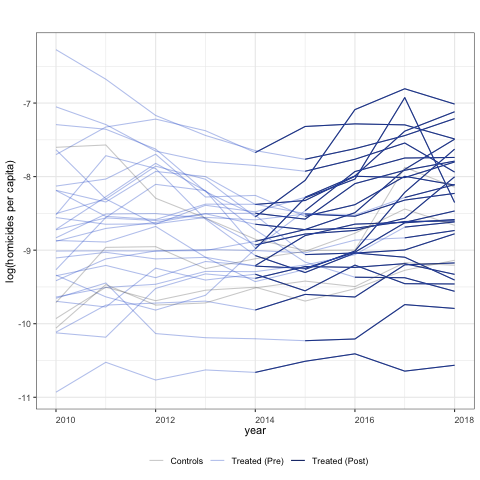
\includegraphics[width=0.9\textwidth]{Figures/reform_treatment_defunciones.png}
       \captionsetup{justification=centering}
\end{figure}    
 
 	

\begin{figure}[h] 
\centering
\caption{Effect of Term Limit Reform of 2014 on Violence \\ -IHS transformation, 95\% confidence intervals-}
\label{fig:event_study_ihs}

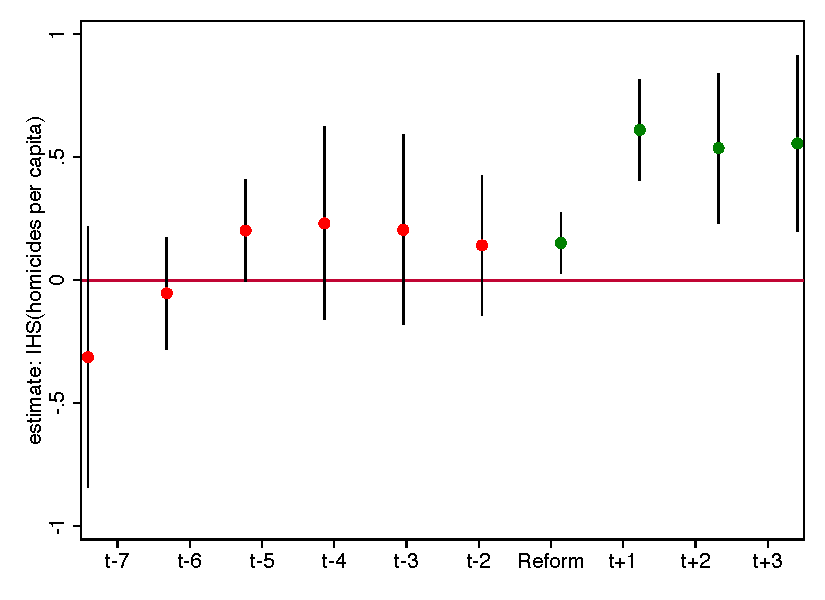
\includegraphics[width=1\textwidth]{Figures/event_study_ihs.pdf}
       \captionsetup{justification=centering}
 Note: Figure \ref{fig:event_study_ihs} shows the IW estimators following \citet{abraham_sun_2020} for each lead and lag relative to the first year a municipality implemented reelection. Red points show pre-treatment estimates, while green ones are post-treatment. 

\end{figure}    
 
  \begin{comment}  
   
 
\begin{figure}[h] 
\centering
\caption{Effect of Electoral Reform of 2014 on Violence \\ -95\% confidence intervals-} 
\label{fig:event_study_ihs}

\begin{center}
	{\textbf Figure A: w/o covariates} 
\end{center}
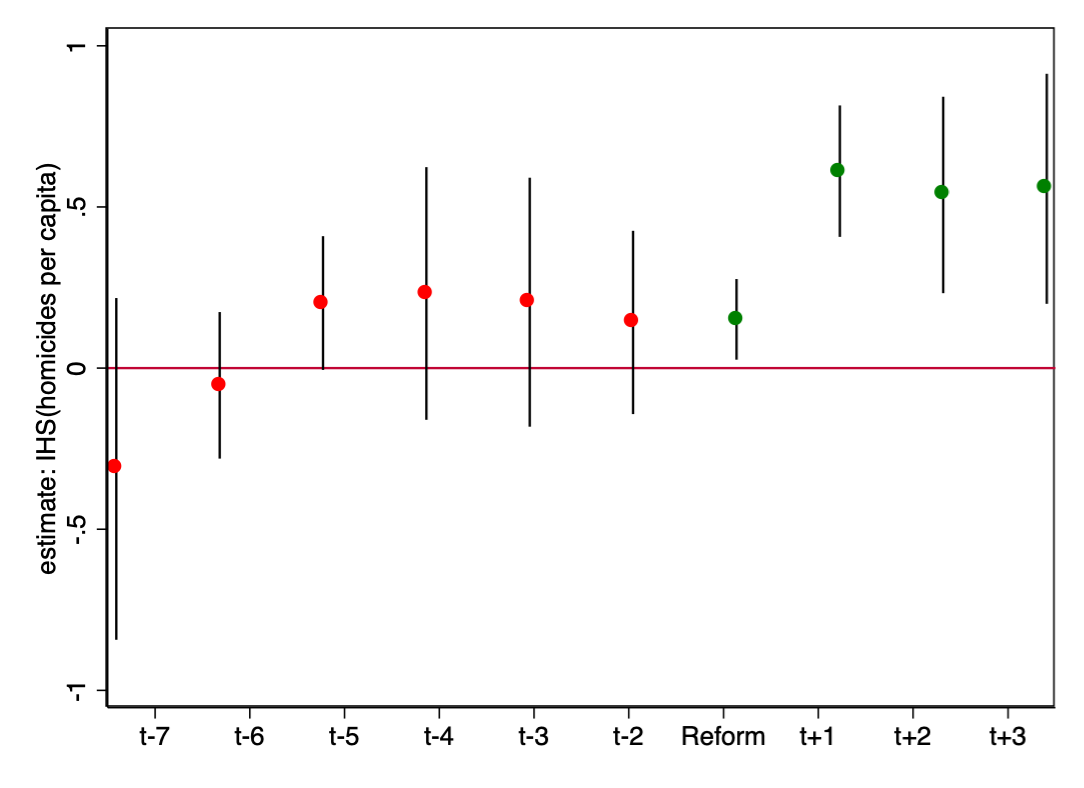
\includegraphics[width=0.6\textwidth]{Figures/event_study_ihs.png}
\begin{center}
	{\textbf Figure B: with covariates} 
\end{center}
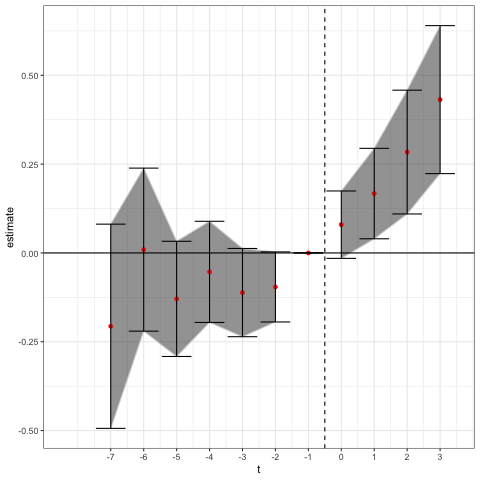
\includegraphics[width=0.6\textwidth]{Figures/event_study_ihs_wcovariates.png}
       \captionsetup{justification=centering}
 \\
 {\textbf Note: I use the inverse hyperbolic transformation sine to transform the dependent variable instead of a natural log. } 
\end{figure}    

 \end{comment}


\clearpage 
 
\begin{comment}
	

\begin{figure}[H]
\centering
\caption{Effect of Electoral Reform on Violence using other methods\\ -95\% confidence intervals-} 
\label{fig:non_did}

\begin{center} 
	{\textbf Figure A: Generalized Synthetic Control following \citet{abraham_sun_2020} }
\end{center}
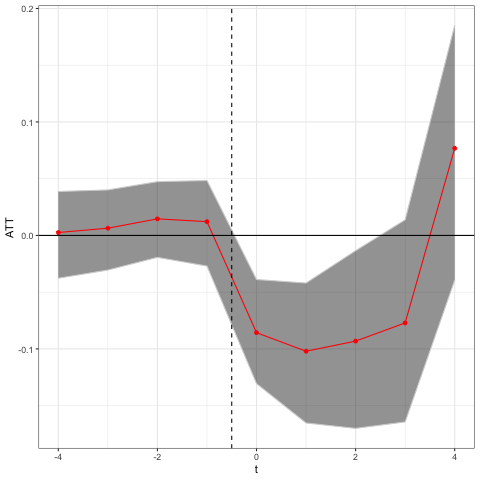
\includegraphics[width=0.55\textwidth]{Figures/gsynth.png}
\begin{center}
	{\textbf Figure B: Matrix Completion following \citet{abraham_sun_2020} }
\end{center}
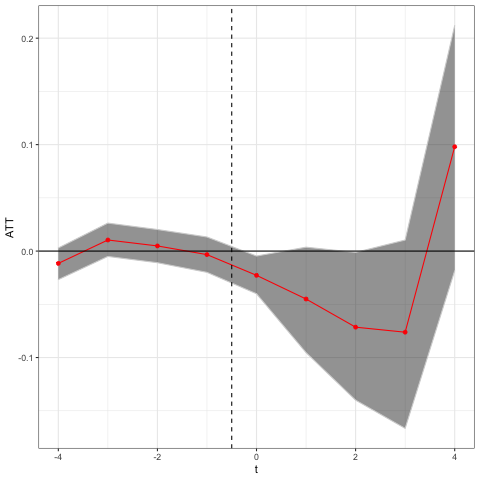
\includegraphics[width=0.55\textwidth]{Figures/matrix_completion.png}
       \captionsetup{justification=centering}
       \\
 %{\textbf Note: .} .   
\end{figure}   
 \end{comment}

\clearpage

\begin{figure}[h]  
\centering
\caption{Sensitivity Analysis for $\theta=\tau_3$ with monotonicity using $\Delta = \Delta^{SDD}(M)$} 
\label{fig:pretrend_violations}

\begin{center} 
	{\textbf Figure A: Monotonically decreasing pre-trend violation}
\end{center} 
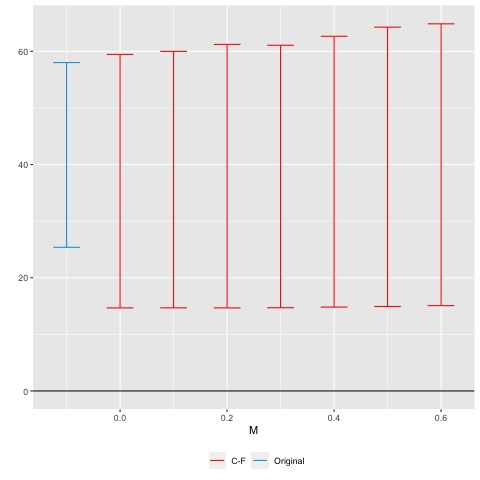
\includegraphics[width=0.55\textwidth]{Figures/pretrends_sensitivity_decreasing.png}
\begin{center}
	{\textbf Figure B: Monotonically increasing pre-trend violation}
\end{center}
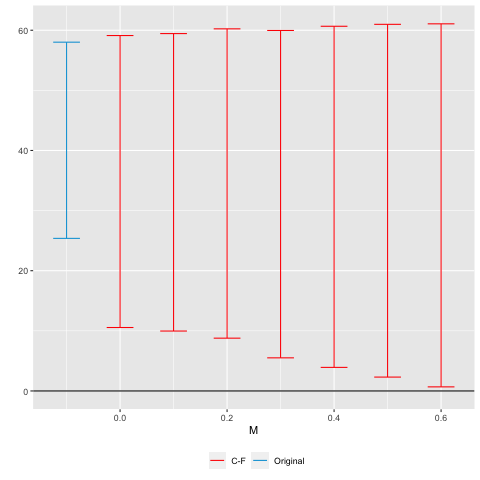
\includegraphics[width=0.55\textwidth]{Figures/pretrends_sensitivity_increasing.png}
       \captionsetup{justification=centering}
       \\  
       
 {\textbf Note: $M$ lower bound=0; $M$ upper bound=0.5536. Blue confidence interval shows the most robust specification of the third lag after treatment in Table \ref{tab:abraham_sun_lagdv} column (2) with a point estimate of 0.4061. C-F stands for conditional fixed length confidence intervals given different values of $M$.} 
\end{figure} 
      
 \clearpage
       



\begin{comment}
	

\begin{figure}[H]
\label{fig:transformations}
\centering
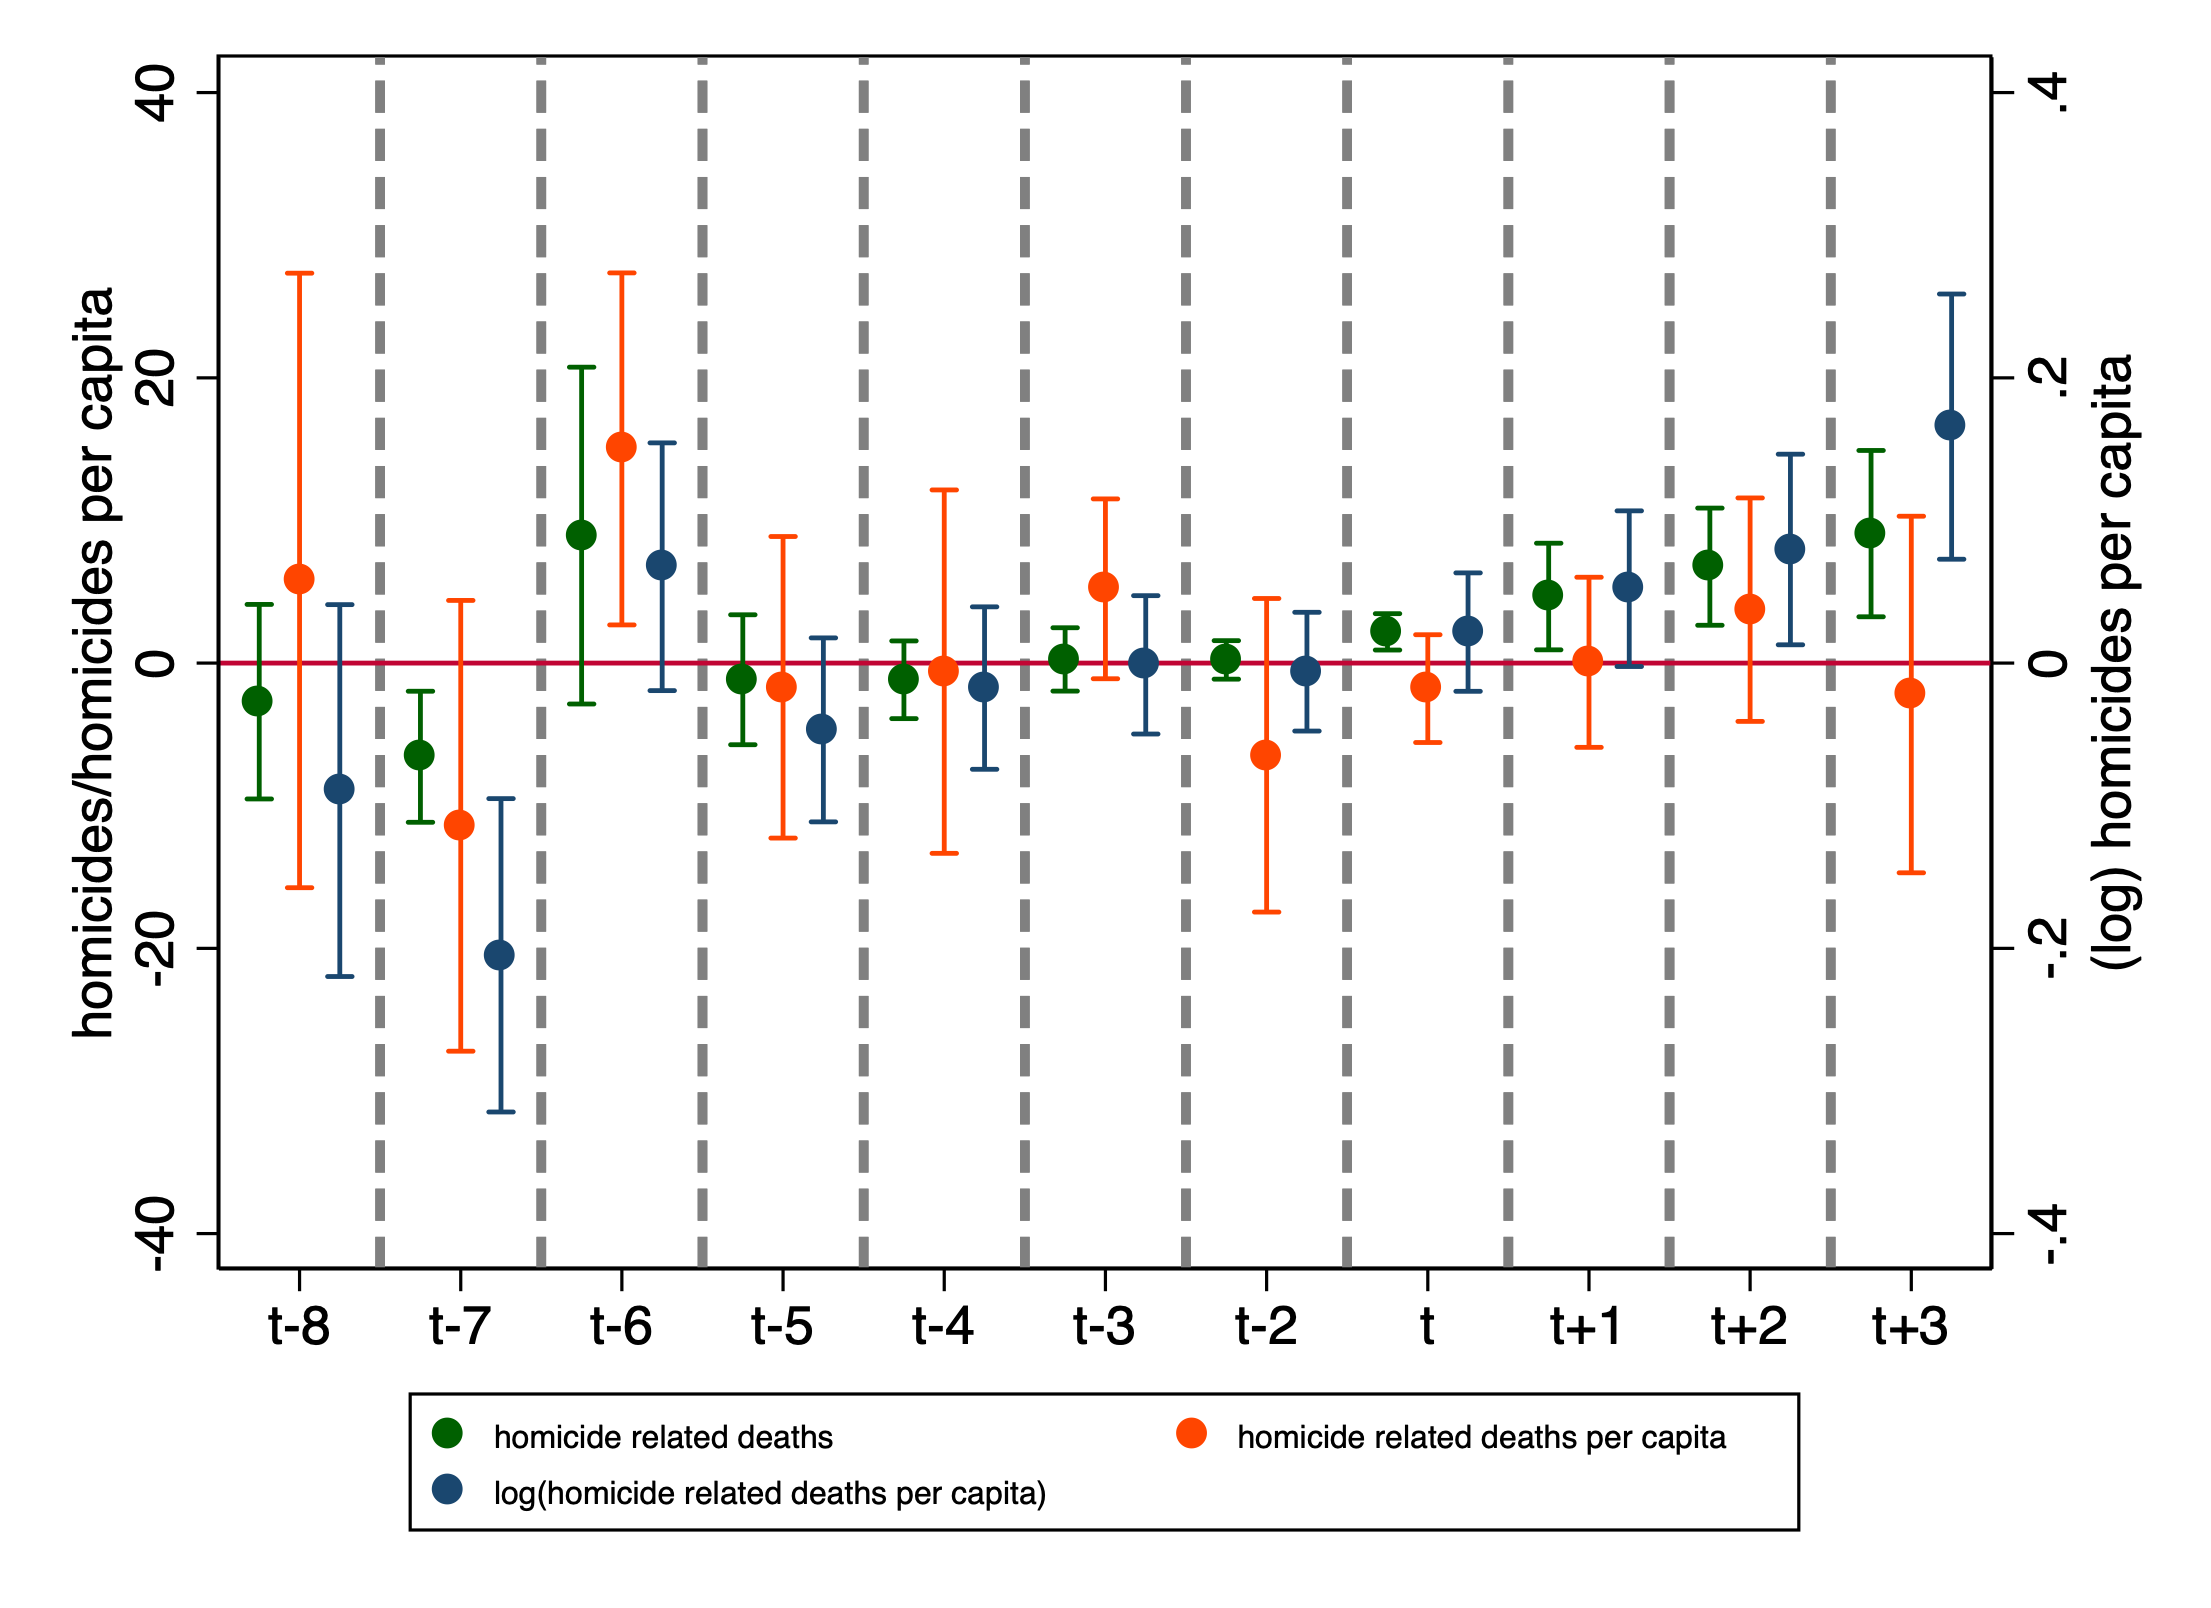
\includegraphics[width=1\textwidth]{Figures/various_transformations_long.png}
       \captionsetup{justification=centering}
\caption{Effect of Electoral Reform of 2014 on Homicides, various DV transformations}
\end{figure}  

\begin{figure}[H]
\label{fig:diff_outcomes}
\centering
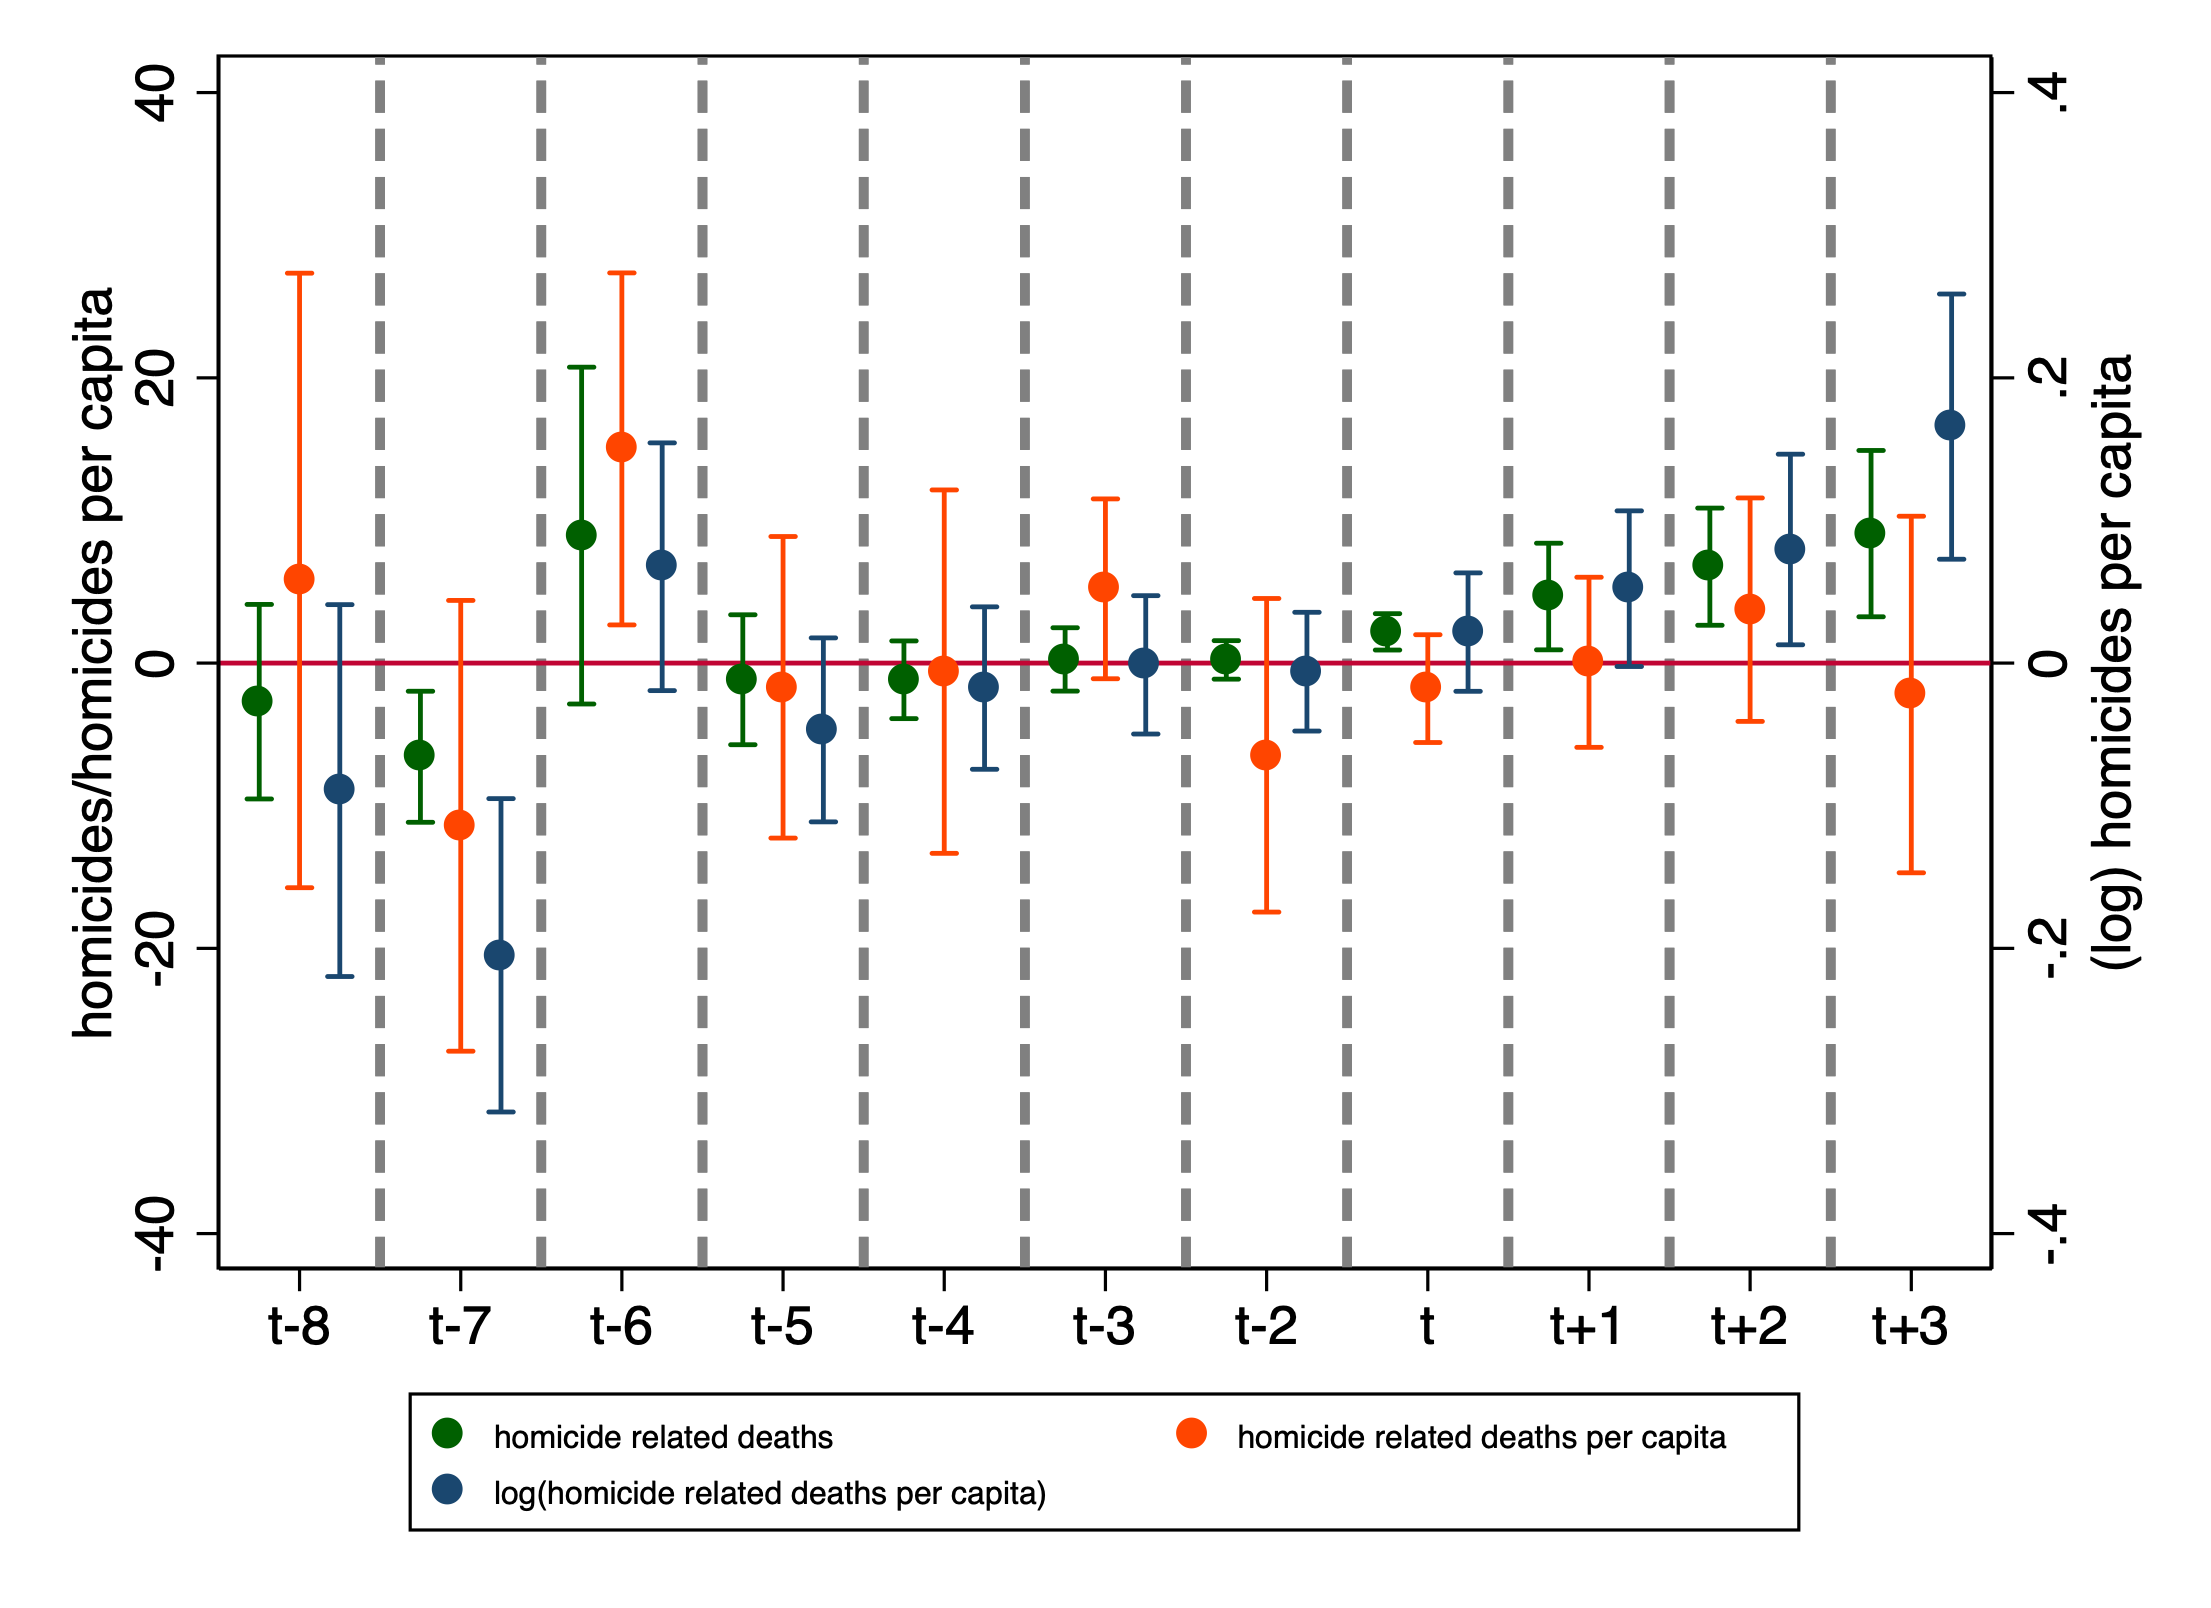
\includegraphics[width=1\textwidth]{Figures/various_transformations_long.png}
       \captionsetup{justification=centering}
\caption{Effect of Electoral Reform of 2014 on Homicides, various outcomes}
\end{figure}   

\begin{figure}[H]
  \label{fig:decomposition}
\centering
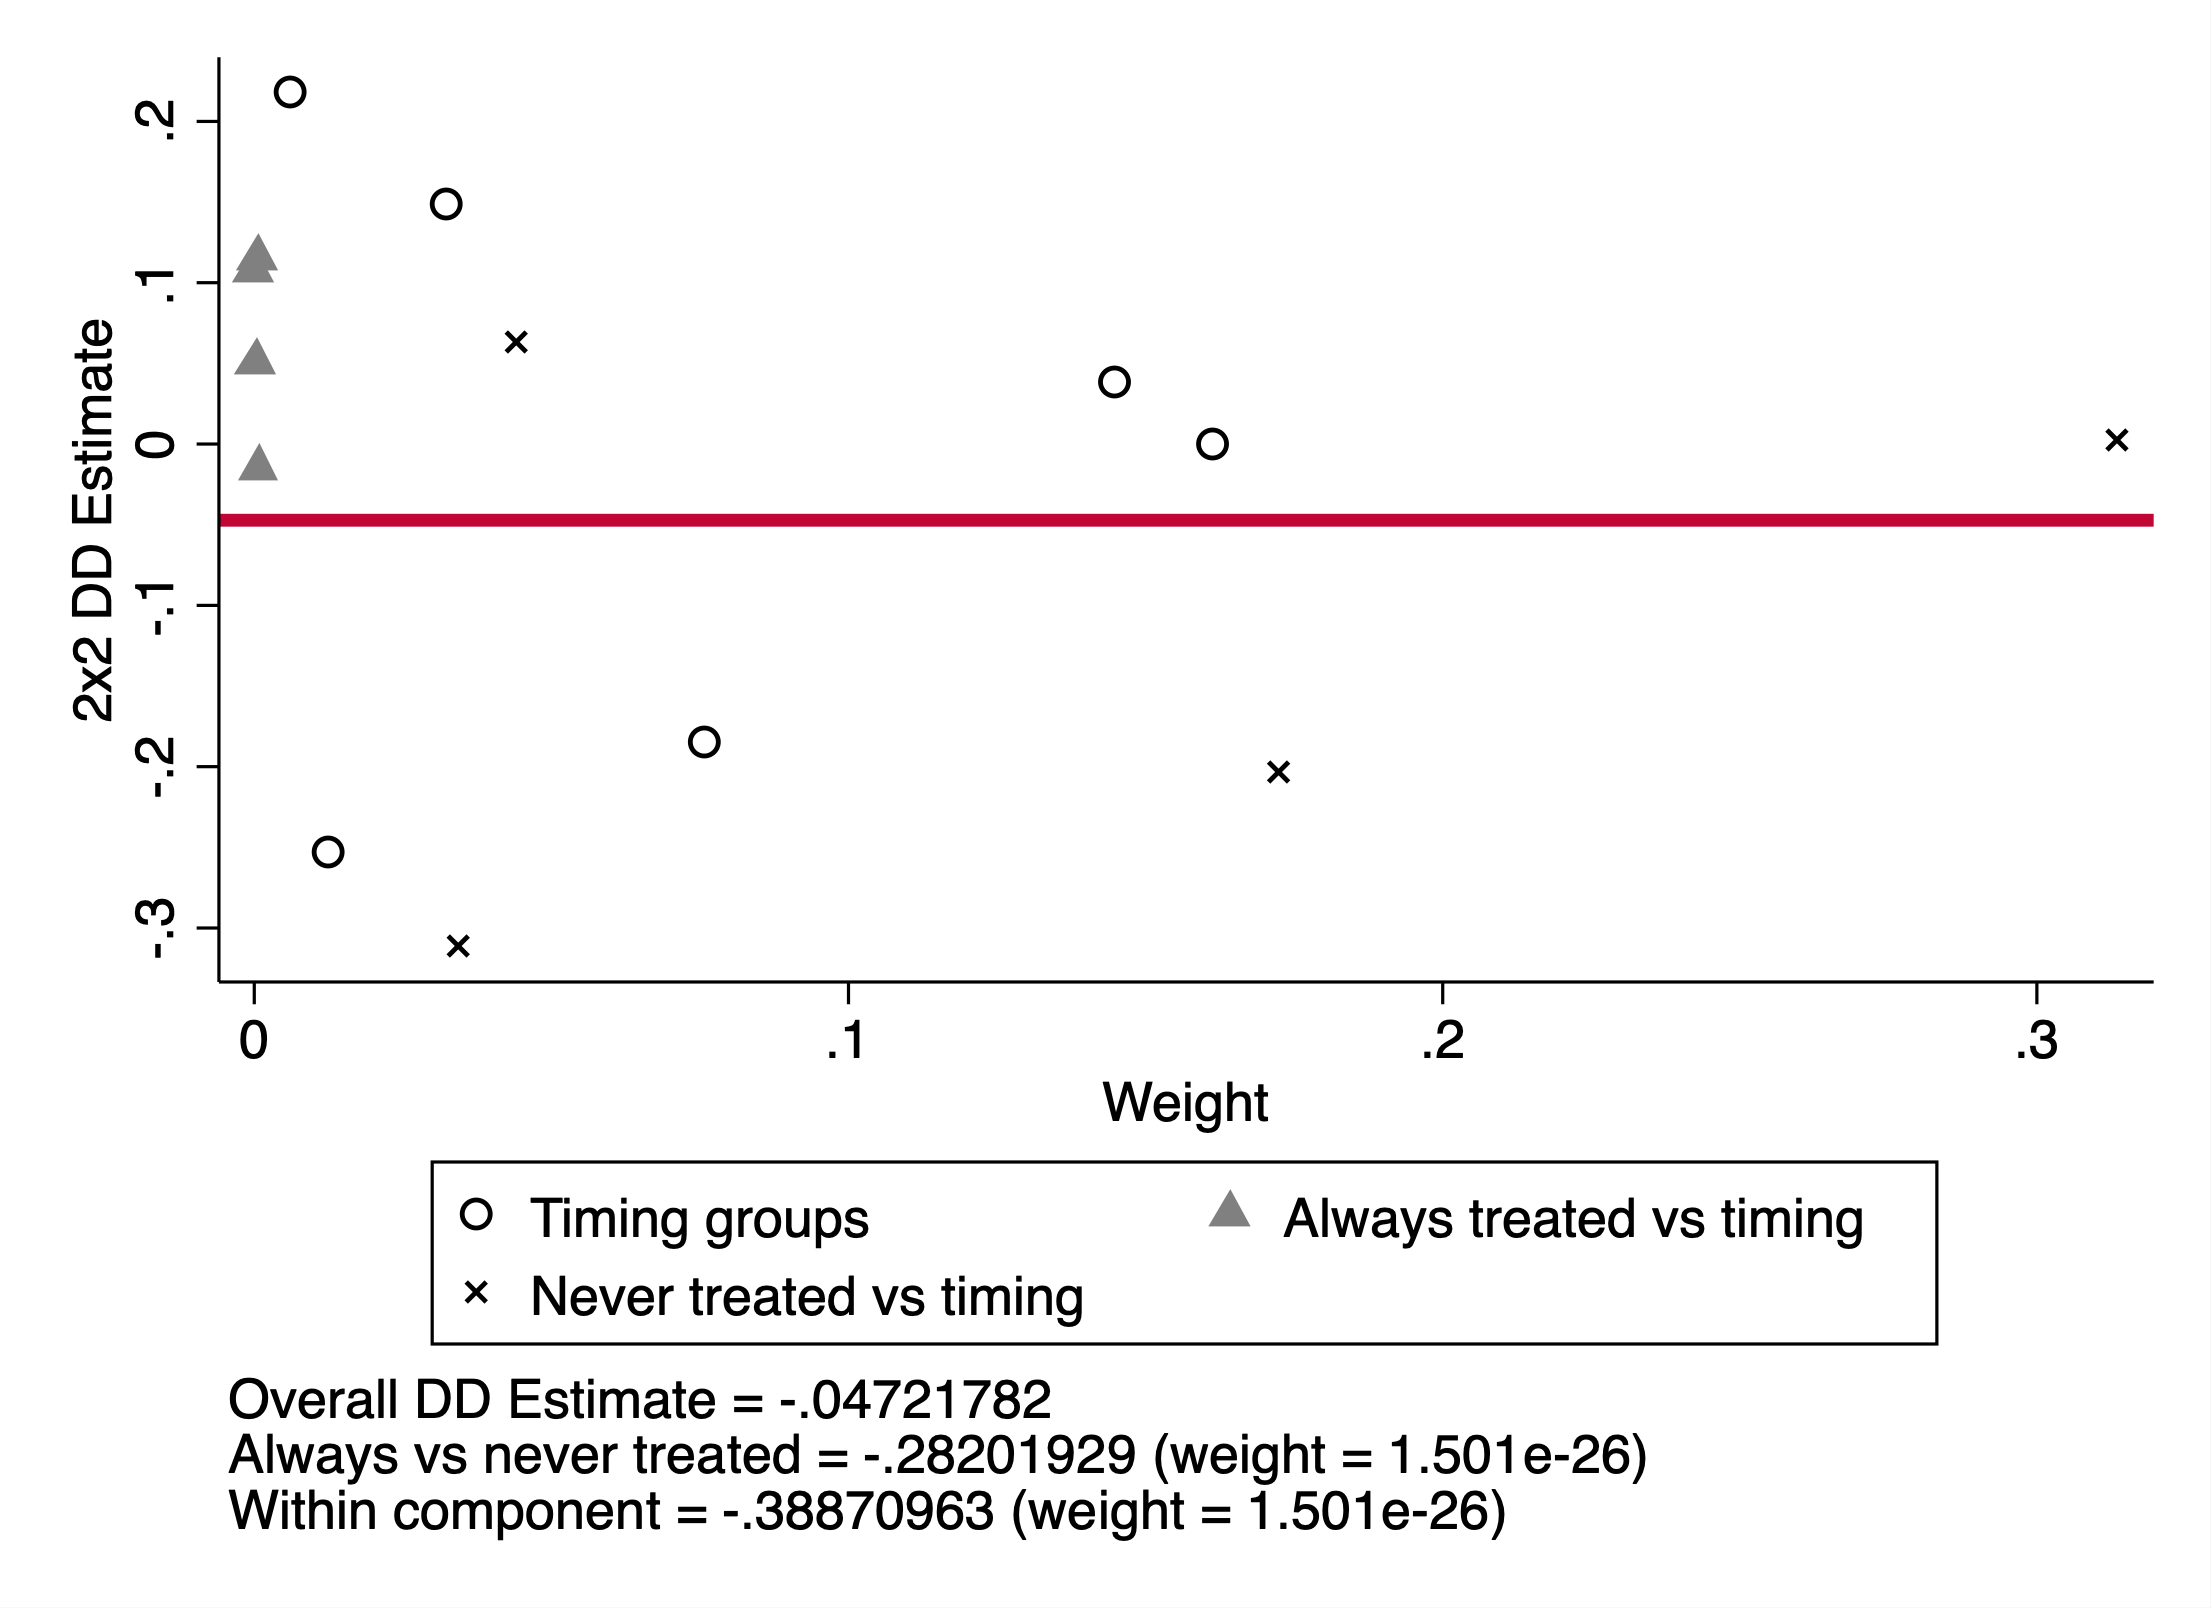
\includegraphics[width=1\textwidth]{Figures/bacon_decomposition_robustSEs.png}
       \captionsetup{justification=centering}
\caption{\citet{goodman_bacon_2018} decomposition}
\end{figure} 

\begin{figure}[H]
  \label{fig:incumbency_event_study}
\centering
\caption{Effect of Electoral Reform of 2014 on Incumbency Advantage}
 
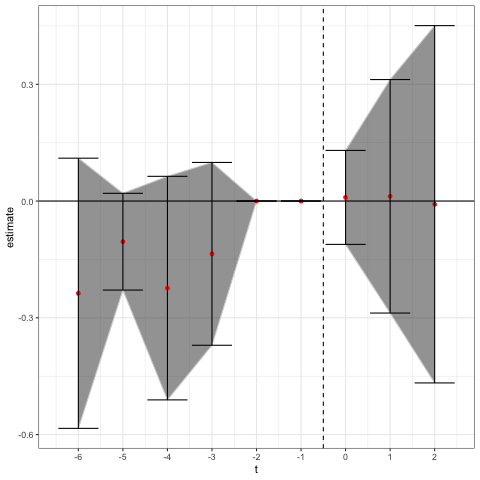
\includegraphics[width=0.8\textwidth]{Figures/event_study_incumbency.png}
       \captionsetup{justification=centering}
\end{figure} 
  \end{comment}
  
  



\begin{figure}[h]  
\centering
\caption{Falsifying Term-Limit Reform Treatment Assignment} 
\label{fig:falsification}

\begin{center} 
	{\textbf Figure A: Pre-treatment}
\end{center} 
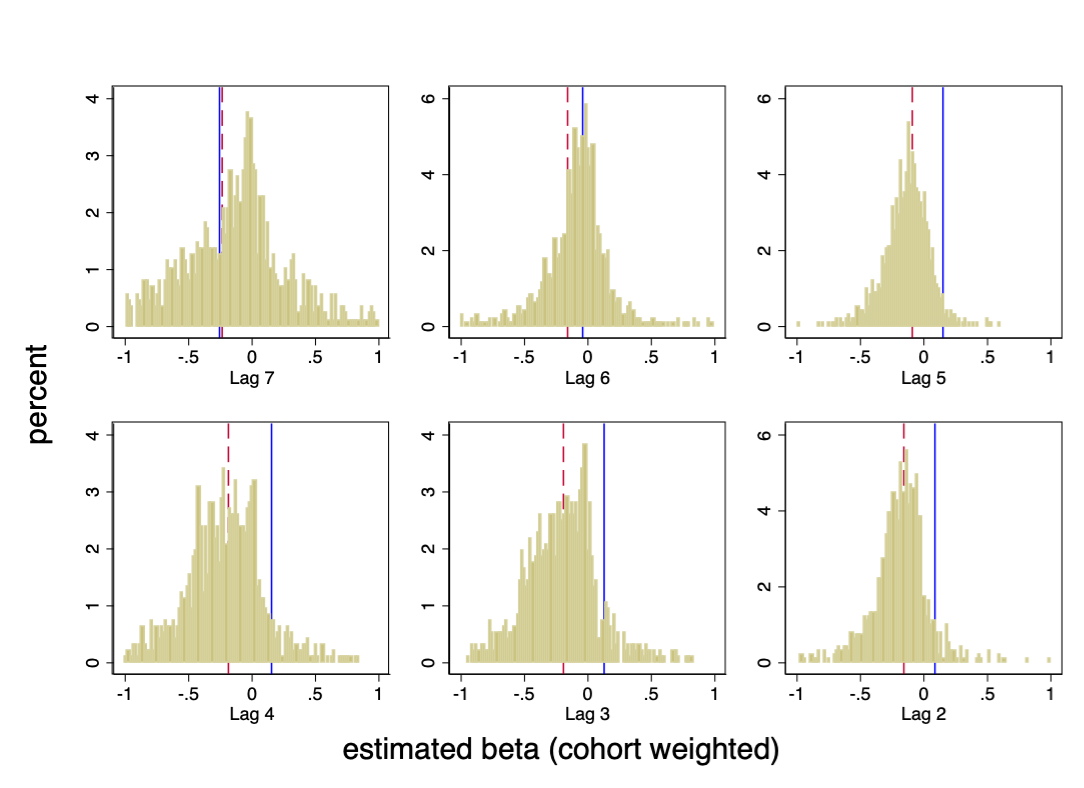
\includegraphics[width=0.8\textwidth]{Figures/falsification_pre2.png}
\begin{center}
	{\textbf Figure B: Post-treatment}
\end{center}
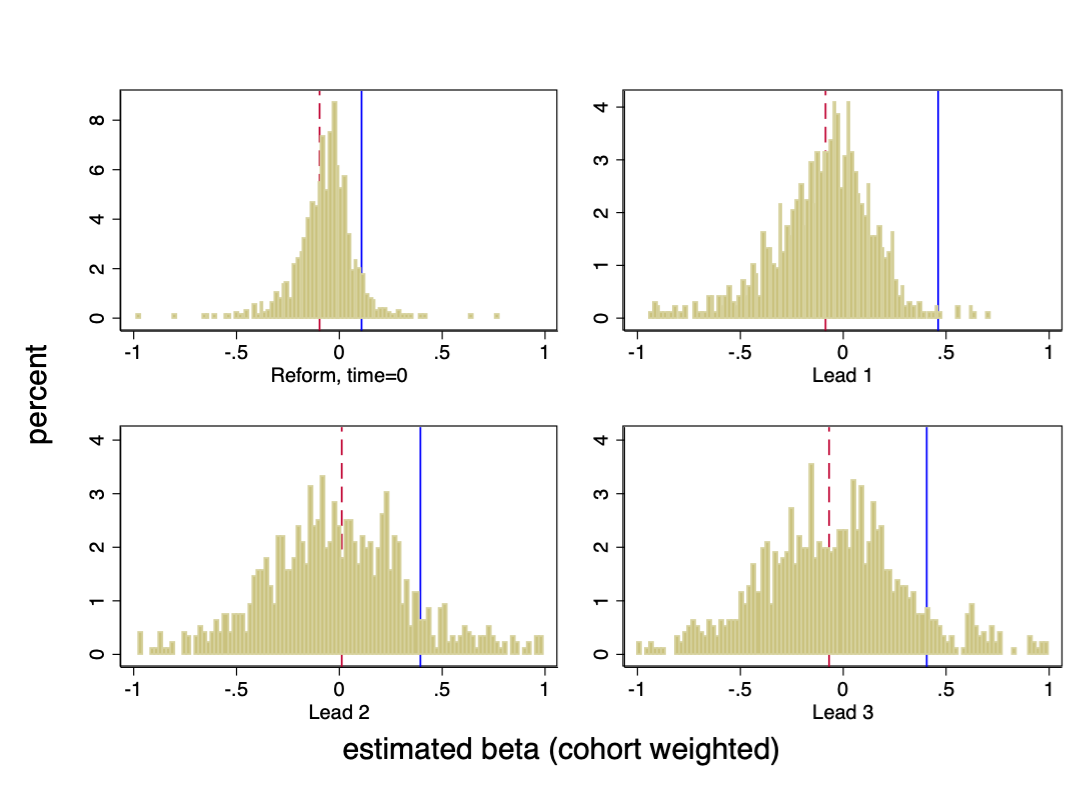
\includegraphics[width=0.8\textwidth]{Figures/falsification_post.png}
       \captionsetup{justification=centering}
       \\  
  {\textbf Note: Estimated (cohort weighted) beta coefficients distribution of 1,000 simulations following equation \ref{eq:abraham}. For each simulation I carry a random Bernoulli draw with success rate equal to the proportion of treated states by the Electoral Reform by time period. Blue line displays the estimated effect of the electoral reform on logged homicides per capita of column (2) o Table \ref{tab:abraham_sun_lagdv}. Red line shows the average estimated effect of the simulations.}     
 
\end{figure}  
   
\clearpage  



\begin{figure}[H]
\centering
\caption{McCrary Test, quadratic polynomial}
  \label{fig:mccrary}

 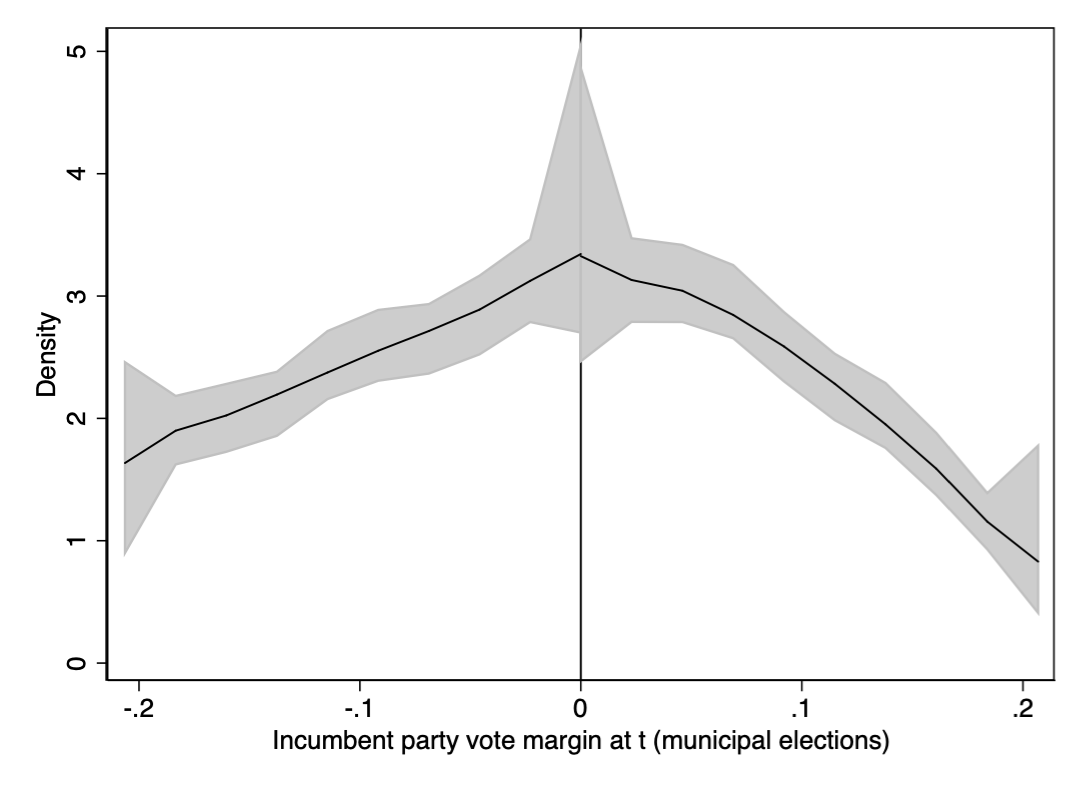
\includegraphics[width=1\textwidth]{Figures/mccrary_test_pol2.png}
       \captionsetup{justification=centering}
 %{\textbf Note: .}     
 
\end{figure} 


    
   
 \clearpage
 
\begin{comment}
\section{George Downs Prize Grant Budget Justification}

Thus far, these results suggest that the vertical accountability of local-level re-election may fail to yield political accountability when accountability from national parties is weak.\footnote{Or accountability from the national executive who's interest is the same as the dominant political party.} A third potential mechanism to explore is the role of political selection. If there is something stressed by the literature on term limit removal, it is the selection of ``good'' candidates to office, or the change in local politician incentives to address citizens interests when their political careers are more dependent on them. However, in Mexico there does not exist a candidate characteristic database to carry on such analysis.   

The George Downs Prize funding will allow for the construction of candidate characteristic database from 2010 to 2019. The database will include data on candidates education level, gender, age, political party and private and public positions hold in the past to proxy experience. With such, a generalized difference-in-difference estimation will allow to test whether the 2014 Mexican Electoral Reform indeed lead to higher voter accountability and politician selection. Also, the database will allow for further research on political selection and state capture.\footnote{Another line of research of mine. See \url{https://papers.ssrn.com/sol3/papers.cfm?abstract_id=3567523}.}   

Specifically, the George Downs Prize will be used to hire two graduate-level research assistants (RAs) to (a) web-scrape municipal candidates from the National System of Municipal Information (\emph{Sistema Nacional de Informaci\'on Municipal)}, (b)  collect candidate-level information from state and municipal-level electoral institutes, (c) security state capacity data, and (d) collect municipal local level covariates spanning from 2010 to 2019 in order to incorporate covariates in a semi-parametric weighting estimator for multi-period difference-in-difference design following \citet{anton_2018}. I expect each RA to work for 60 hours, at an hourly rate of USD \$16.00, i.e. a total of USD \$1,920.00 ($=60*2*16$). Their work will help me reach August 2020 with a full version of the paper, and have a final draft ready to present at APSA 2020. 
 \end{comment}
 
  \clearpage 
  
%%%%%%%%% Scope condidtions

\section{Scope conditions \label{sec:scope}} 

I leverage the staggered implementation of the 2014 Electoral Reform in Mexico  to test the effect that reelection incentives had on violence as a proxy of welfare, and public security provision as a proxy for incumbents performance in office (for details on the War on Drugs see Section \ref{sec:war} and on the Reform see Section \ref{sec:reform}). Mexico has specific traits that make it an ideal case to study the disconnection between reelection and political accountability. Furthermore, these characteristics help in the identification of the effect of the reform on violence and public security provision.

First, the War on Drugs that started in December 2006 after former President Felipe Calderon's military intervention agains DTOs in the state of Michoacan, generated substantial violence and drug trafficking activity across states, municipalities and time (see Figure \ref{fig:homicides_evolution} on state-level homicides variation across time). Second, there is strong decentralization in the provision of public security. Since 2006 the military -army and marine forces- led the battle against DTOs. Locally, however, public security provision is in charge of municipal police forces, alongside state and federal police bodies for specific cases. A third characteristic is Mexico's strong party system and strong parties. Following \citet{mainwaring_scully_1995}, Mexico's party system is strong due to the stability pattern of competition (mainly a three party system during the last 30 years), strong partisanship in society, constant and legitimate elections -even during the autocratic totalitarian party-system; see \citet{magaloni_2009}-, and strong hierarchical party organization, i.e. the strong capacity parties have to constraint party members behavior. Furthermore, the central government in Mexico has various degrees of delegation of public security to mayors. Likewise, political parties have various degrees of delegation in terms of local electoral strategies and clienteles targeting. Deviation from party lines, however, is punished through removal of nomination candidacy. In a system where party switching is existing but small, party whip is strong both a the local executive level and local and federal legislatures. This party strength is found in both big and small parties. Thus, Mexico provides a case with parties with the capacity to monitor its members, but not necessarily the willingness to do it given electoral and clientelistic incentives.  

As noted by \citet{schedler_2001}, the democratic transition in Mexico since 2000 led paradoxically to the strengthening of clientelistic activities in Mexico, particularly in rural areas. As a result of the PRI of loosing the Presidency to the right-wing PAN in 2000 and 2006, and multiple legislative and local level elections since, the PRI shifted to vote buying behavior and different forms of clientelism. Moreover, with fiscal decentralization reforms from the early 90s, state and municipal executives developed clientelistic practices in exchange of federal funds, following party line \citep{cornelius_2002}. These funds allowed for the expansion of local clientelistic networks, a dynamic deeply studied by \citet{larreguy_2013}.

%It is important to note that prior to 2000, the President in Mexico hold metaconstitutional powers: he controlled the Federal Executive, was appointed the \emph{de facto} head of the majoritarian party, and was the chair of the candidate nomination committee. As a result extreme discipline was forced not only from the leadership of the party but from the presidential office \citep{weldon_1997}. After 2000, the majoritarian party the PRI lost the presidency and till 2012 lost control of the lower house in Congress. As a result, a PRI president no longer sat in the candidate nomination committee of the PRI. It was till 2017 that a PRI President, Pena Nieto, led again the Permanent Political Commission in charge of selecting every single candidate of the PRI.  
 
Fourthly, to avoid problematics in terms of identification related to heterogeneity in the preference of public goods, Mexico provides a case with an  overwhelming demand for a specific good, peace, with potential variation in the degree of public security provision. Throughout the study time period from 2010 to 2018, violence is the primary concern in the country. In Section \ref{sec:alternative_voter_demand} I explore the role of differential public security demands from citizens, given that they may prefer peace across the country, but only public security deployment away rather than at home given strong externalities on fighting crime.   
 
In short, we are facing a specific context: Mexico, characterized by high variation in crime and public security provision, a political environment with strong clientelistic parties, one mayor public good of interest -peace-, and legitimate democratic institutions.  

%Diagram: voters and parties. Agent. Two things affect it: (a) relative strength and (b) degree of oversight. (a) is affected by institutional framework of either, reelection and winning margin. (b) is affected by whether they are strong or weak, again affected by reelection and the institutional framework. Cases: (i) voter > party, (ii) party>voter, and (iii) same force. Cases of (b): (i) voter oversight > party oversight; (ii) party oversight > voter oversight; (iii) same. I cannot differentiate but can know what happens with overall effect. there can be (i) and (i) then we have greater public good provision and welfare; (i) and (ii) or (ii) and (i) then it depends. and equal, then its mixed too. But very important, if strong party then voters can use reelection to measure incumbents performance. Then incumbency advantage, that decreases incumbent party incentive. 
\clearpage

%%%%%%%%% Electoral Reform 2014
\section{Political Background of the 2014 Electoral Reform}\label{appendix:reform_backgorund}


It is important to understand the electoral reform political motivation, which involved a bargaining process with the opposition as well as the incorporation of pending laws from the political reform of 2012 under the PAN presidency. In the last year of Felipe Calderon presidency, a political reform was introduced in Congress including a term limit removal for all political actors. This reform was proposed and introduced during the electoral period of that year, increasing political tensions among the incumbent and opposition parties. The PRI -at the time part of the opposition and in control of the lower legislative house- blocked the reform and targeted reelection and the introduction of a second electoral round for the presidential election. 
 
  The 2012 presidential election was won by the coalition ``Alliance for Mexico'' with its presidential candidate Enrique Peña Nieto.\footnote{The PRI won with 38.2\% of total votes, followed by the PRD with 32.6\% and the PAN with 25.390\%.} However, the election suffered multiple electoral irregularities exposed by the national media. Among anomalies, opposition parties led by Andres Manuel Lopez Obrador -the second runner of presidential election and at the time presidential candidate for the left-wing party PRD-, argued PRI's financial expenses above campaign caps and vote-buying practices including the distribution of gift cards from several institutions, including one of the country's largest supermarket chains, Soriana, to voters in the State of Mexico and Mexico city. \citet{cantu_2019} finds not only an effect of the gift cards in PRI electoral return, but a magnitude that increases given proximity of electoral precincts to stores. While the special commission in the Chamber of Deputies found that the PRI invested \$5,200 million pesos in the campaign, an amount 15 times larger than the finance cap of \$336 million pesos, and the Inspection Unit from the Federal Electoral Institute (IFE for its acronym in Spanish) detailed the financing network where Soriana, Banamex, Monex and other firms where involved, the Unit did not point to any law violation. Without a public discussion, the ministers of the Federation Judicial Electoral Tribunal (TEPJF for its acronym in Spanish) deemed the appeal filed by the PRD unfounded and endorsed IFE's  criterion that the PRI was not obliged to register the agreement with Soriana, Banamex or Monex as campaign expenses.\footnote{In his presentation, magistrate Manuel Gonzalez Oropeza stated that the analysis carried by the Inspection Unit showed that ``neither the allegedly hidden financing was accredited individually or jointly" by any member of the PRI. See \url{https://www.jornada.com.mx/2013/01/24/politica/013n2pol} for more detail.} The final resolution of IFE's Council and the TEPJF increased citizens and opposition mistrust on electoral institutions. 

By early 2013, the Pena Nieto administration pushed an aggressive set of reforms to privatize the energy sector and modify the existent fiscal institutions in the country. To increase the probability of success, the PRI with the PAN and PRD, the three main political parties at the time, lead the construction of the Mexican Pact Accord, a series of roundtables intended to negotiate the energy sector reform along a set of structural reforms that had fail to pass through congress due to political gridlocks.\footnote{The PRD was no longer under the Lopez Obrador leadership who left the party to build a new left-wing party called MORENA once the leaders from the PRD agreed to form part of the Mexican Pact Accord.} While the Electoral Reform was not under PRI's set of desired reforms, the opposition utilize it as a bargaining chip to approve those pursued by the PRI \citep{zamitiz_2017}. By the end of May 2013, a roundtable to discuss the electoral reform was installed. Specifically, commitment 94 of the Pact Accord introduced reelection for discussion. However, due to lack of consensus, the Mexican Pact Accord did not submit an electoral reform proposal to Congress and left the bargaining process to the Senate. Two months later, on July 24, 2013, PAN and PRD pushed a political-electoral reform with 36 law changes that included  the creation of a National Electoral Institute (INE for its acronym in Spanish) that would be in charge of federal, state and local elections and reelection for federal and local legislators and mayors. In the words of the current Chairman of the INE, Lorenzo Cordova, ``[w]ith the reform, we went from an electoral model made up of a federal electoral system and thirty-two electoral systems, to a national election system in which a national authority and thirty-two local authorities coexist; a national administrative body was created, with clear powers and powers for local elections, and an authority was created that coordinates and guarantees the same parameters for the application of laws by local authorities, in order to standardize the conditions of the electoral competition in all elections and to promote a more transparent and impartial democracy throughout the country€.\footnote{From Cfr. Compendio de Legislacion Nacional Electoral, Mexico, INE, FEPADE, UNAM, TEPJF, Tomo II, 2014, p. XXXIX.} 


The reaction of governors was not smooth since reelection would limit the influence of governors and local elites on the electoral processes of the 32 states. Strong governors like the priista Eruviel Avila Villegas from the State of Mexico labeled this initiative as ``democratic regression".\footnote{For more detail see ``Regresion democratica, creacion del Instituto Nacional de Elecciones€, La Jornada, 30 de octubre, 2013, p. 15. \url{https://www.20minutos.com.mx/noticia/b82075/regresion-democratica-creacion-del-instituto-nacional-de-elecciones/}} Given the state-level opposition, Senate leaders from the PAN and PRD chose to approve the electoral reform in December 2, 2013, before the energy reform, and thus increased their political grip over the PRI.\footnote{The electoral reform approved by the Senate included reelection for federal legislators and governors for up to 12 years, as well as reelection for local legislators and mayors. Congress, however, modified the proposal removing governors reelection. The electoral reform was approved with 408 votes in favor and 69 against in Congress on December 3, 2013, and weeks later by the Senate due to modifications of the original reform project.} By January 2014, PAN and PRD threatened to back the energy reform  if the PRI did not push local state legislatures from approving the electoral reform, a constraint imposed by the Mexican constitution, which at the time where blocking the reform given pressure from various PRI governors.\footnote{For more detail see Enrique Mendez, ``PAN: estancados, cambios en materia politica por presion de los gobernadores€, La Jornada, 9 de enero de 2014, p. 5., \url{https://jornada.com.mx/2014/01/09/politica/005n3pol}.} The political gridlock led former President Pena Nieto to ``exhort" local legislators to approve the electoral reform. On January 31, 2014, the reform was promulgated by the President and contained three main changes: (1) the creation of the INE; (2) removal of term limits of mayors, local and federal legislators for up to 2 terms; (3) the introduction of a ``party-lock"	where mayors or legislators who wish to reelected could not switch parties. As a result, while voter accountability increased, party control remained unchanged since candidate nominations and campaign funding still depended strongly on them. 
 \clearpage 
  
%%%%%%%%% SNSP
\section{Sistema Nacional de Seguridad P\'ublica Homicide Database}\label{appendix:SNSP_homicides}
   
The Sistema Nacional de Seguridad P\'ublica Homicide Database database is fed by the reports of local prosecutors offices. Thus it inherits the same flaw of INEGI's second homicide database counting cases rather than victims. The difference is that INEGI reports figures in an annual basis (and a six month delay) while the SNSP reports data in a monthly to monthly basis. In 2015, the SNSP updated their methodology to classify homicide related criminal investigations.\footnote{The new methodology allows to differentiate crimes against women, and add complementary information from emergency numbers 911. There is no agreement if data captured through the new methodology can be paired with the old one due to differences in the filing of criminal cases.} This new methodology captured data from 2015 onwards, while the old methodology stopped capturing data in 2018. Two problems arise with the SNSP database, however. First, given the data collection effort to produce monthly estimates, there is high data inaccuracy. Second, this inaccuracy is tied to governors' political agenda. \citet{ch_rivera_2013} note, for example, a crime rate drop of 28\% three months prior to the governor election of Veracruz in 2010. Three months after the election, cases with pre-election date are added by the end of that year. Noteworthy, this pre-election decrease in homicides is not observed in INEGI's homicide related deaths database.  States manipulate statistics so the story is the one governors want to tell.
  
 \clearpage
 
%%%% NO ANTICIPATORY ASSUMPTION   
\section{Validating the no-anticipatory assumption \label{appendix:CDLZ}}


One way to address the no-anticipatory behavior is to assume that it can only occur in a fixed window prior to the electoral reform, say of one year, especially since the reform was announced in early 2013. However, for states that implemented reelection later this fixed window assumption would not suffice. In other words, only those early adopters of the reform would show unbiased estimates. Late adopters, however, would anticipate the term limit removal an act accordingly biasing the results upwardly.  
 
Another way to assess the no-anticipatory behavior from incumbents in this setting is test whether early vs late adopters differed in their estimated effects. Appendix Figure \ref{fig:CDLZ} presents \citet{cengiz_etal_2019} ``event-by-event analysis" that estimates treatment effects for each treated Mexican state (28 states) in the sample. States color differs if they are early (2015-2016, red color) or late adopters (2017-2018, blue color). Specifically, I create state-event specific panel datasets and estimate state-specific estimates using separate regressions for each state. Each state dataset contains the treated state and all other states that never received treatment or received treatment after the sample window of $t+1$. For each state I estimate the following DiD regression: 

\begin{equation}
y_{mt}=\mu_m	 + \mu_t + \gamma Reform_{mt} + \epsilon_{mt}
\end{equation}

where $Reform_{mt}$ is an indicator variable that takes the value of 1 if the state implemented reelection. If there was evidence of strong incumbent anticipatory behavior, conditional on state covariates such as governor winning margin and alignment with Federal Executive, we would expect strong color clustering across similar estimated effects. In other words, if there is an endogenous response by states to implement the electoral reform, we would see that the positive (or negative) treatment effect would be only by those that implemented reelection earlier or later (events with the same color would be clustered). However, as seen in Appendix Figure \ref{fig:CDLZ}, this is not the case: there is wide variation in estimated coefficients across early (red) and late (blue) adopters of the reform, conditional and unconditional on state covariates.    

Given the proportion of states with null-effects (16 out of 28) in  Figure \ref{fig:CDLZ}, we could be concerned that the average treatment effect of all these events would yield null results. For robustness, Appendix Figure \ref{fig:stacked_wcontrols} presents the ``stacked dataset analysis" from \citet{cengiz_etal_2019}. I take each of the ``event-by-event'' datasets from Figure \ref{fig:CDLZ}, stack estimates by cohort and estimate one set of lead and lag variables not using prior treated units as controls. Panel B shows that conditional on state-level covariates, there is strong evidence of pretrends as well as strong positive effect of reelection on logged homicides per capita. While there might be evidence of an increasing dynamic trend, it disappears if we include the lag of the main outcome.\footnote{Results available upon request.}  

     
\begin{figure}[H]
\centering
\caption{``Event-by-event analysis'' following \citet{cengiz_etal_2019}\\ -95\% confidence intervals-} 
\label{fig:CDLZ}

\begin{center} 
	{\textbf Figure A: w/o covariates }
\end{center}
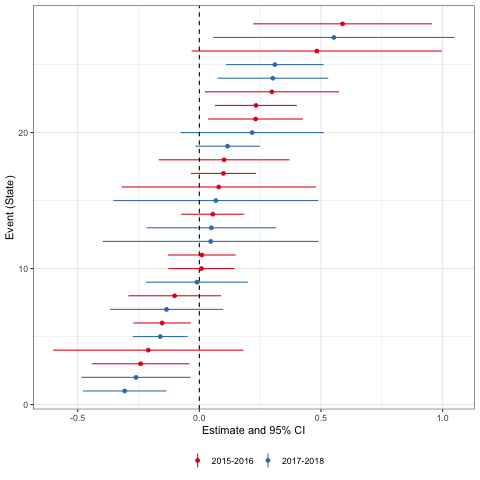
\includegraphics[width=0.4\textwidth]{Figures/CDLZ.png}
\begin{center} 
	{\textbf Figure B: with covariates } 
\end{center}
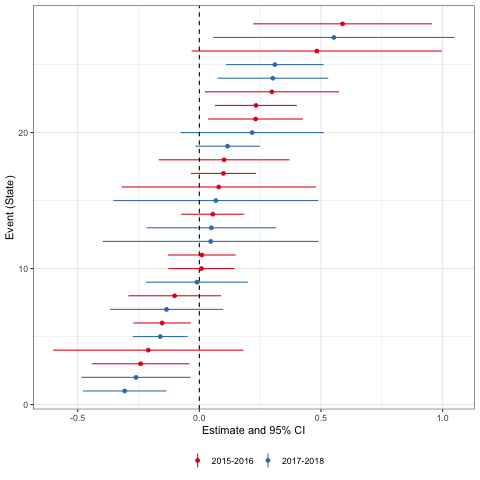
\includegraphics[width=0.4\textwidth]{Figures/CDLZ_cov.png}
       \captionsetup{justification=centering}
       \\
 {\textbf Note:} Estimate separate treatment effects for each event, i.e. each Mexican state in the sample. Each event dataset contains the treated state and all other states that never received treatment or received treatment after the sample window ($t+1$).   
\end{figure}    

\begin{figure}[H]
\centering
\caption{``Stacked dataset analysis'' following \citet{cengiz_etal_2019}\\ -95\% confidence intervals-} 
\label{fig:stacked_wcontrols}

\begin{center} 
	{\textbf Figure A: w/o covariates} 
\end{center}
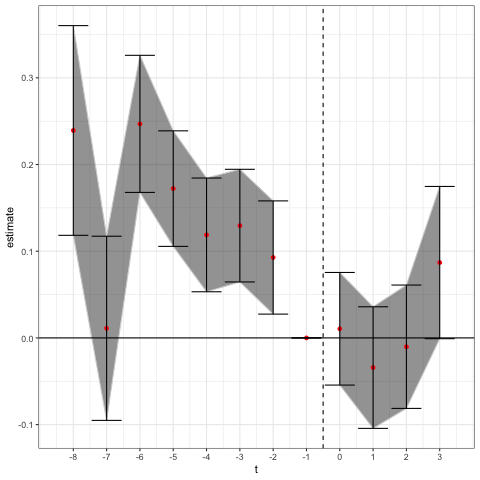
\includegraphics[width=0.55\textwidth]{Figures/stacked_dataset.png}
\begin{center}
	{\textbfFigure B: with covariates} 
\end{center}
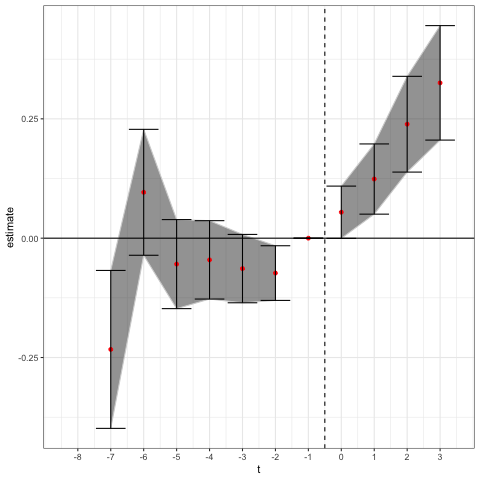
\includegraphics[width=0.55\textwidth]{Figures/stacked_dataset_wcontrols.png}
       \captionsetup{justification=centering}
       \\
 {\textbf Note: Utilize estimated coefficients from Figure \ref{fig:CDLZ} and stack them in relative time, and estimate lead and lag variables to treatment following the event-by-event analysis setup, i.e. without treatment containment from using prior treated units of controls. Analysis done stacking at the cohort level, and adding municipality and year fixed effects.}   
\end{figure}   


%%%SENSITIVITY ANALYSIS

\section{Sensitivity Analysis on violations to the parallel trends assumption \label{appendix:sensitivity}}

As an additional robustness check on parallel trends, Figure \ref{fig:pretrends_sensitivity} reports confidence sets under different assumptions about the set of possible violations of parallel trends following \citet{rambachan_roth_2019}. This allows the reader to evaluate what assumptions need to be imposed in order to obtain informative inference in this setting. In particular, I set $\Delta$ -i.e. a set of possible differential trends-\footnote{$\Delta=\{0\}$ in the presence of pretrends, for example.} equal to $\Delta^{SD}(M)$ that relaxes the assumption of linear differences in trends by stating that the slope of the differential trend among treated and non-treated municipalities can change by no more than $M$ in consecutive periods. Figure \ref{fig:pretrends_sensitivity} shows robust confidence sets at different values of $M$ for the third lag after treatment.\footnote{Similar results are found for the first year of treatment, as well as one and two lags after. Results available upon request.} I calibrate $M$ through benchmarking, that is from the largest change in slope between periods among non-treated states, and use this as the upper bound of the interval to benchmark $M$. In this case $M$ upper bound is equal to 0.5536. As noted in Figure \ref{fig:pretrends_sensitivity}, we can reject the null hypothesis equal to zero even if we allow for changes in slope more than 0.55 times as large as the upper bound for the largest changes observed for the placebo group. In other words, when we allow for linear violations of parallel trends the figure does not change dramatically and intervals do not touch 0.  

\begin{figure}[!htbp]  
\centering
\caption{Sensitivity Analysis for $\theta=\tau_3$ using $\Delta = \Delta^{SD}(M)$} 
\label{fig:pretrends_sensitivity}

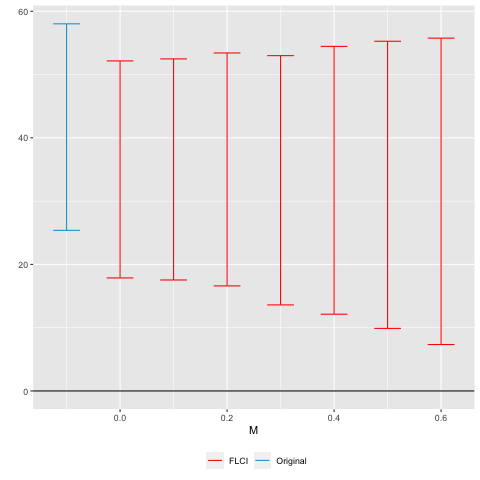
\includegraphics[width=0.7\textwidth]{Figures/pretrends_sensitivity.png}
       \captionsetup{justification=centering}
\bigskip  

{\textbf Note: $M$ lower bound=0; $M$ upper bound=0.5536. Blue confidence interval shows the third lag after treatment in Table \ref{tab:abraham_sun_lagdv} column (1) with a point estimate of 40.61\%. FLCI stands for fixed length confidence intervals given different values of $M$.} 
\end{figure}  
   
Now, I incorporate context specific knowledge into the restrictions used in the sensitivity analysis. Appendix Figure \ref{fig:pretrend_violations} develops such exercise and carries a similar exercise to that shown in Figure \ref{fig:pretrends_sensitivity}, but imposing that violations of parallel trend be (weakly) decreasing (panel A) or increasing (panel B). For the former, prior to the Electoral Reform, we notice a downward-sloping pre-trend in homicides. %(see Figure \ref{fig:event_study_wcovariates}, for instance). 
It may be valid to assume that such trend would have continued absent treatment. Thus, we could impose a negative shape restriction, i.e. a monotonically decreasing one. For the latter, we assume that pre-trend violation follows and upward slope where homicides would increase in treated states relative to control ones. In such setting, those that enacted the Electoral Reform in earlier years would have done so if they thought the reform would be a policy instrument to tackle such violent setting. In both cases (monotonically decreasing and increasing) the lower bound of the robust confidence never touches 0 (null effect), increasing assurance on the found estimates with the OLS specification. In both Figure A and B, a positive effect of reelection on logged homicides per capita is found, across multiple values of M including its upper bound. Furthermore, with the added monotonicity restrictions, the lower bound of the robust confidence in Panel A (B) falls below the lower bound of the OLS confidence interval. This is intuitive, since the restriction that is decreasing (increasing) implies that the OLS coefficient is weakly upward bias.

\clearpage 

%%%% RDD design
\section{Regression Discontinuity Design of close elections, before and after the Term Limit Removal Reform of 2014 \label{appendix:rdd}} 

I begin by visualizing the effect of the reform on incumbency advantage.  Figure \ref{fig:incumbency_advantage} presents the RDD estimate of close elections on incumbency advantage  within an optimal bandwidth distance $h$ from the cutoff (0), and a quadratic polynomial:\footnote{A triangular kernel is used. Results are almost unchanged when using other polynomial functional forms.} Panel A shows a comparison of municipalities with incumbents at $t-1$ that barely won to those that barely lost in $t$ on the probability of electoral victory at $t+1$,\footnote{Incumbency advantage measure following \citet{klasnja_titiunik_2017}.} taking into account all elections from 1979 to 2014 (i.e. prior to the term-limit reform); Panel B shows the same comparison but restricting the sample to municipalities that implemented reelection after 2014. I do not consider those municipal elections that after 2014 did not implement reelection. Table \ref{tab:rdd} shows RD estimates using multiple polynomial functional forms. Even though RD estimates are biased in this setting, especially for Panel B in Figure \ref{fig:incumbency_advantage} (and even columns in Table \ref{tab:rdd}) since in the presence of staggered treatment timing and heterogeneous treatment effects across cohorts are not causally interpretable since we are considering both early vs late adopters of the reform on the treated,\footnote{The next iteration of this working paper will show this proof in the Appendix for RD designs.} they provide a striking depiction of what occurred before and after the electoral reform. 


\begin{figure}[H]
\centering
\caption{Effect of Term Limit Reform of 2014 on Incumbency Advantage, quadratic polynomial}
  \label{fig:incumbency_advantage} 

	%{\textbf Figure A: quadratic polynomial}
 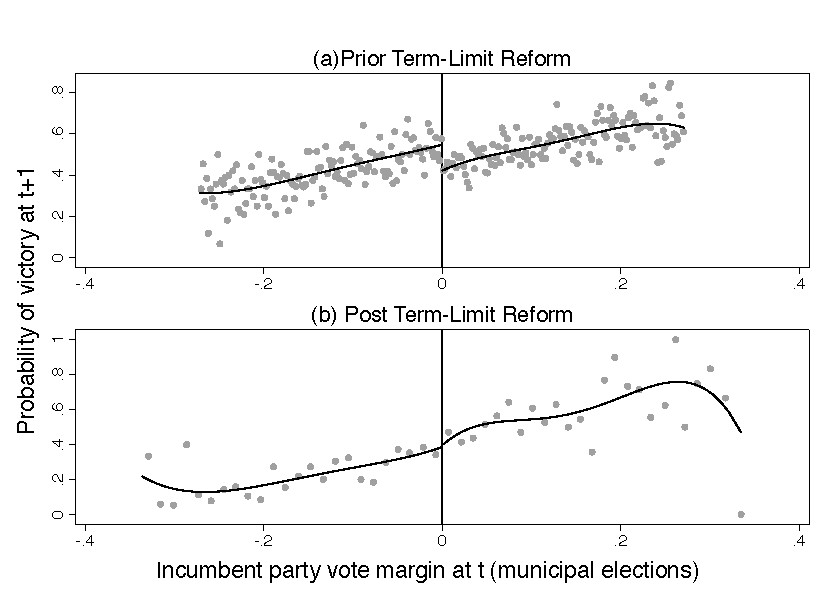
\includegraphics[width=1\textwidth]{Figures/RDD_incumbency_pol2.pdf}
     \captionsetup{justification=centering}  
       
\end{figure} 
       Note: Regression Discontinuity design of close elections on incumbency advantage. Panel (a) considers all elections from 1979 to 2014. Panel (b) considers all elections after 2014 for municipalities that implemented reelection.) 
\\
       
Before the reform, there was a negative statistical significant difference between municipalities that barely won and lost on the probability of success in the next election. This incumbency \emph{disadvantage} aligns strongly with a similar result found by \citet{klasnja_titiunik_2017} for the case of Mexico. \citet{klasnja_titiunik_2017} find that an incumbent party that is barely reelected suffers a reduction in the probability of winning the following election of 28 percentage points. In contrast, I find a reduction between 10.7 to 11.32 percentage points, a finding that considers 20 more years of elections since \citet{klasnja_titiunik_2017} cap their data from 1997 to 2009, while I consider elections since 1979 to 2014. 

More interesting is the finding that after reelection takes place the previous incumbency disadvantage disappears as noted by a positive and non-statistical significant difference between municipalities that barely lost and won an election. This initial RDD results provide suggestive evidence that the electoral reform generated an increase in the probability of victory in the next election for municipalities that barely won an election relative to those that barely lost. The next section addressed potential biases and presents robust findings of this same evidence.  


 \\ 
  
%Table:
\begin{table}[!htbp]\def\sym#1{\ifmmode^{#1}\else\(^{#1}\)\fi}
\caption{Regression Discontinuity Design of Close Elections on Incumbency Advantage, comparing pre and post-Term Limit Reform estimates}
\label{tab:rdd}
\begin{center} 
\scalebox{0.7}{
\begin{tabular}{lcccccccc}
 
\hline \hline   
\\
   
\multicolumn{9}{l}{Dependent variable:}\\
  
\\
            &\multicolumn{2}{c}{linear polynomial}      &\multicolumn{2}{c}{quadratic polynomial}   &\multicolumn{2}{c}{}                       &\multicolumn{2}{c}{}                       \\\cmidrule(lr){2-3}\cmidrule(lr){4-5}\cmidrule(lr){6-7}\cmidrule(lr){8-9}
            &\multicolumn{1}{c}{(1)}         &\multicolumn{1}{c}{(2)}         &\multicolumn{1}{c}{(3)}         &\multicolumn{1}{c}{(4)}         &\multicolumn{1}{c}{(5)}         &\multicolumn{1}{c}{(6)}         &\multicolumn{1}{c}{(7)}         &\multicolumn{1}{c}{(8)}         \\
\addlinespace
Conditional Probability of victory at t+1&      0.1138\sym{***}&      0.0640         &     -0.1074\sym{***}&      0.0724         &      0.1130\sym{***}&      0.0500         &     -0.1119\sym{***}&      0.0562         \\
            &    (0.0220)         &    (0.0711)         &    (0.0217)         &    (0.0635)         &    (0.0245)         &    (0.0863)         &    (0.0274)         &    (0.0845)         \\
\addlinespace
Observations&       8,026         &         711         &       8,622         &         888         &      11,255         &         897         &      10,125         &         956         \\
Post Reform (2014)&                     &  \checkmark         &                     &  \checkmark         &                     &  \checkmark         &                     &  \checkmark         \\
 
 
        
\hline \hline   
\multicolumn{9}{p{1.3\textwidth}}{\footnotesize{Notes: Standard errors in parentheses, with the following significance-level: $^{***}$ 1\%; $^{**}$ 5\%; and $^*$ 10\%, that refer to two-sided t-test. Optimal bandwidth following \citet{calonicoetal_2014} $^a$ Incumbency advantage measured following \citet{klasnja_titiunik_2017}. 
  }} \\  
\end{tabular}         
}
\end{center} 
\end{table} 

\clearpage

%%%% Ruling out the signing of centralization agreements

\section{\emph{Wash one's hands} of security provision \label{appendix:acuerdos}}%\label{sec:wash_hands}}

\begin{flushright}
	``I am innocent of the blood of this just person: see ye to it.'' \\
	 Pontious Pilate, Matthew 27:24, King James Version.  
\end{flushright}
\bigskip

An alternative mediator to the increase of violence is local executives refusing to take responsibility or be involved any further in the provision of public security. With reelection, non-term limited incumbents may choose to sign security cooperation agreements with upper administrative levels, including those with the state or the federal government. Some of these agreements may imply a full delegation of public security provision to governors or the president. In other words, mayors in line for reelection would \emph{wash their hands of} public security provision to refuse to take blame for violence. Those new in charge -governors or the President- may decrease public good provision or see an increase in violence since they are misinformed of local crime and how to deter it \citep{berman_lake_2019} or are simply not willing to tackle it given party electoral incentives describe in Section \ref{sec:mechanism}.

Since the presidency of Felipe Calderon (PAN, 2006-2012), there have been five broad types of security agreements between municipalities and upper level governments: (a) agreements between municipalities (e.g. to create metropolitan police forces), (b) between municipalities and the state governor (e.g. Central Command Agreements), (c) between municipalities and the federal government, (d) agreements with multiplicity of executive actors (various municipalities, states, with or without the Federal government), and (e) agreements with other branches of government, including legislative and judicial ones, also at various levels of government. While conditions vary by agreement, overall they may include any (or all) of the following items: security coordination, transit, security prevention, training, sharing of equipment and technology, research capacity, analysis and intelligence, and creation of unified criteria and procedures of the public security institutions and laws. 

Of all agreements, the creation of a state-level Police Central Commands (\emph{Mando \'Unico Policial}) has been the most prevalent in Mexico. The premise is the unification of municipal and state police forces, i.e. the centralization of public security under direction of the governor. During Calderon's presidency, Central Commands were intended to abolish municipal police forces. Later, Pena Nieto's administration proposed the creation of Unified State Forces to transition from 1,800 municipal police bodies to 32 police corporations. However, a proposed constitutional modification was stopped in the Senate since it did not reached the necessary three quarters of legislators to approve the Constitutional modification. While it did not achieve constitutional jurisdiction, by 2018 79.12\% of municipalities in the country adopted a form of centralized command according to data from the 2019 National Census of Municipal Governments and Territories of the City of Mexico.\footnote{There is a judicial discussion in Mexico on the legitimacy of centralized state level agreements, particularly that of the Centralized Command. In the framework of the Mexican federal pact, Article 21 of the Constitution that makes public ministries (\emph{Miniserios P\'ublicos}) the actor in charge of prosecution. However, they are  left aside in most security cooperation agreements. Furthermore the Constitutional figure of the ``free municipality'', makes public security centralization something unfeasible and unconstitutional \citep{moloeznik_2016}. As noted by Article 115, fraction III, item ``h" of the Constitution, municipalities are the first autonomous constitutional bodies and are granted express powers to provide public security service. For more details see \url{https://aristeguinoticias.com/0608/mexico/el-inconstitucional-mando-unico-articulo/}.}  

Appendix Figure \ref{fig:mando_unico} shows that the Term Limit Reform did not increase the likelihood of municipalities on signing security cooperation agreements. Prior to treatment we observe pretrends. Once the reform is implemented there is actually a decrease in the probability of signing an agreement, but non-significant. For those municipalities with four years of implementation we see an increase in the likelihood of having an agreement, but it is quite noisy.\footnote{For robustness, Appendix Figure \ref{fig:controlling_mando_unico} shows main estimates on the effect of the reform on violence robust to controlling for security cooperation agreement.}   

Now, while there is no effect of reelection on mayors refusing to take care of public security matters, we would expect that municipalities without Police Central Command (or other cooperation agreements) would experience lower welfare distortions (i.e. lower violence) since they would be hold more accountable by citizens on local security provision. This is exactly what we find. Appendix Figure \ref{fig:split_mando_unico} estimates the effect of the Term Limit Reform on logged homicides per capita on two subsamples: one the one hand, municipalities with security agreements prior to the implementation of the Reform (points with black lines representing 95\% confidence intervals); on the other hand, municipalities without such agreements (squares with dashed lines representing 95\% confidence intervals). As noted, both subsamples show positive effects of the reform on violence, with the exception of the first year of treatment for those without security cooperation agreements. More importantly, there is significant difference between both subsamples for all the years after the reform was implemented: municipalities with security cooperation agreements such as \emph{Mando \'Unico Policial} show a higher increase in the percentage of homicides per capita in treated municipalities relative to non-treated. 

One important concern could arise: why don't we see a null effect on municipalities without security agreements? %Is not bottom-up voter accountability biting? 
Would not these municipalities serve as placebos? To answer this there are three important caveats about security cooperation agreements -particularly Central Command Agreements- that needs to be noted. 

First, not all Central Command Agreements imply a \emph{de jure} delegation of municipal public security provision to the state. There is wide variation of what central command implies, and could take all or any of the items mentioned before, from security provision to intelligence. In other words, \emph{Mando \'Unico} in one state may not imply the same operative features in another state.  %Second, even if there is complete \emph{de jure} delegation of public security from mayors to governors (or the Federal Government), \emph{de facto} there are various degrees in which public security is provided. 
For instance, as noted by data from the National Census of Municipal Governments and Territories of the City of Mexico from 2011 to 2019, of all the municipalities that state they had a Central Command Agreement, only 72.6\% said the agreement included the delegation of public security.

Second, even with the existence of a security cooperation agreements that delegates all security provision to higher level federal authorities, citizens could still blame mayors for not lobbying federal authorities for public good provision in their municipalities. Moreover, citizens may simply not understand the terms and conditions of cooperation agreements, blaming mayors still for local level violence. Lastly, \emph{Mando \'Unico Policial} has not led to a decrease in crime incidence, especially since municipal police forces require a distinct training and objectives to those of states \citep{david_lopez_2018}, and has been deemed as either non-existent or a failure.\footnote{For more detail, see the article ``Mando \'Unico Policial: el modelo fracasado" from \url{https://www.proceso.com.mx/515386/mando-unico-policial-el-modelo-fracasado}} Given these caveats, municipalities without security cooperation agreements should not be deemed as placebos, but should show a significant difference in the level of violence as found in Appendix Figure \ref{fig:split_mando_unico}. 
 
 
  \begin{figure}[H]
\centering
\caption{Effect of Term Limit Reform on Probability of Signing a Security Cooperation Agreement}
  \label{fig:mando_unico}

 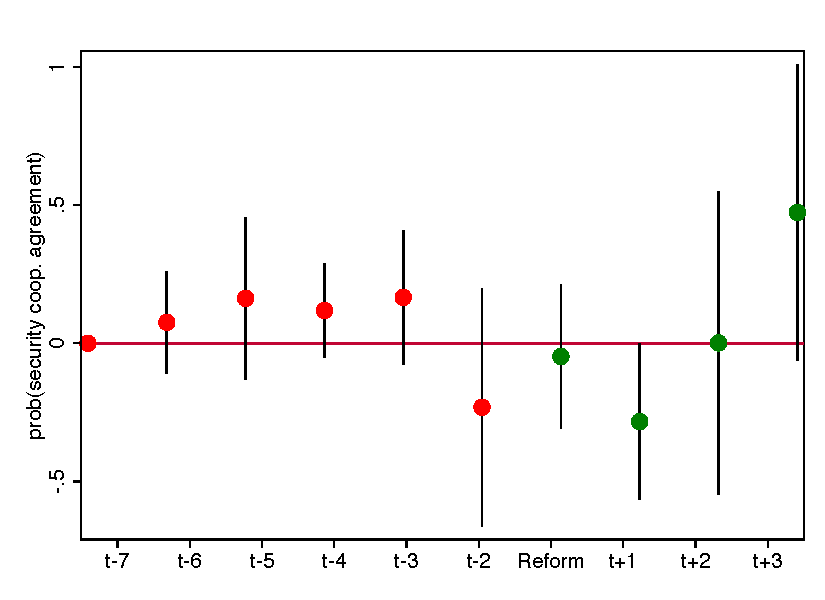
\includegraphics[width=1\textwidth]{Figures/mando_unico.pdf}
       \captionsetup{justification=centering}
 {\textbf Note: Figures shows the estimates of equation \ref{eq:abraham} using as outcome an indicator variable of whether a municipality signed a security cooperation agreement according to information from the National Census of Municipal Governments and Territories of the City of Mexico, 2011-2019. The Figure shows IW estimators with 95\% confidence intervals.} 
 
\end{figure}  

 \begin{figure}[H]
\centering
\caption{Effect of Term Limit Reform on Violence, conditional on Signing a Security Cooperation Agreement}
  \label{fig:controlling_mando_unico}

 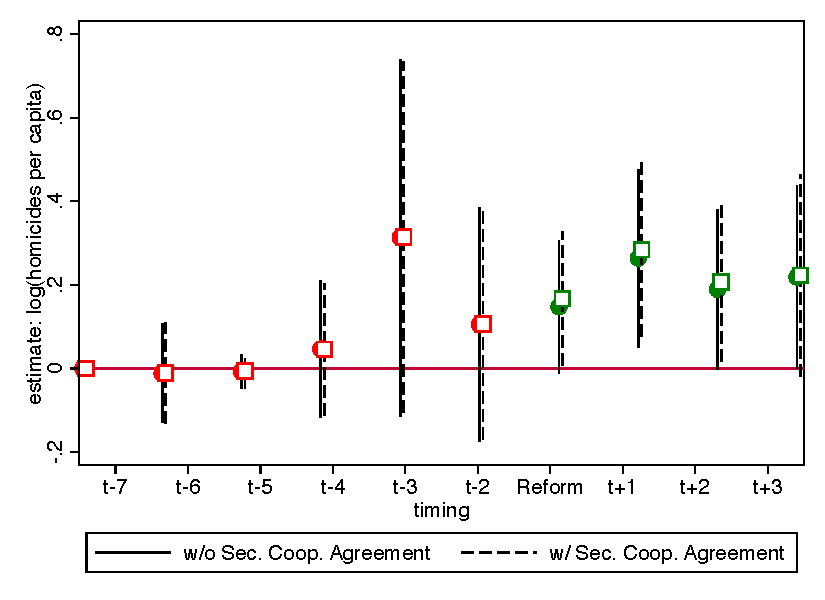
\includegraphics[width=1\textwidth]{Figures/controlling_mando_unico_log.pdf}
       \captionsetup{justification=centering}
 {\textbf Note: Figures shows the estimates of equation \ref{eq:abraham} conditional on whether a municipality signed a security cooperation agreement one year prior to treatment according to information from the National Census of Municipal Governments and Territories of the City of Mexico, 2011-2019. The Figure shows IW estimators with 95\% confidence intervals.}    
   
\end{figure} 
    
 
\begin{figure}[h]  
\centering
\caption{Effect of Term Limit Reform on Violence, by security cooperation agreement} 
\label{fig:split_mando_unico}

   
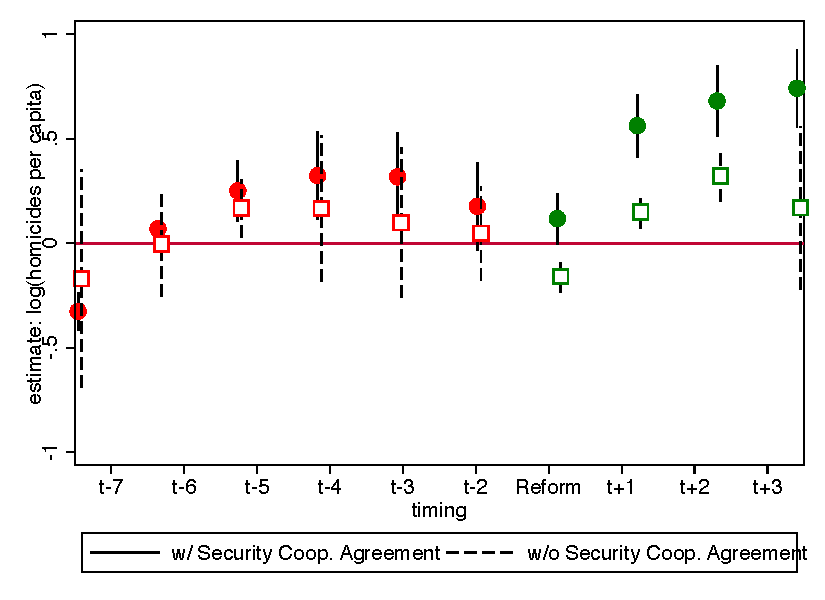
\includegraphics[width=1\textwidth]{Figures/event_study_w&wo_placebo.pdf}
  
 {\textbf Note: Line shows estimates for the subset of municipalities with a security cooperation agreement prior to treatment. Dashed line shows estimates for the subset of municipalities without a security cooperation agreement prior to treatment. The Figure shows IW estimators with 95\% confidence intervals.} 
\end{figure} 

\clearpage

%%%%%%%%%%%%%%%%%%%%%%%%%%%%%%%%%%%%%%%%%%%%%%%%%%%%%
\section{New Tables and Story \label{appendix:new_tables}} 
%%%%%%%%%%%%%%%%%%%%%%%%%%%%%%%%%%%%%%%%%%%%%%%%%%%%%
\renewcommand{\thetable}{J-\arabic{table}}
\setcounter{table}{0}
 
\renewcommand{\thefigure}{J-\arabic{figure}}
\setcounter{figure}{0}
%%%%%%%%%%%%%%%%%%%%%%%%%%%%%%%%%%%%%%%%%%%%%%%%%%%%%

%Table
\begin{comment}
\begin{table}[htbp]\def\sym#1{\ifmmode^{#1}\else\(^{#1}\)\fi}
\centering
\caption{Effect of Centralization of Public Security on Violence}
\label{tab:centralization_homicides}
\scalebox{0.8}{
\begin{tabular}{lcccc}
\hline \hline
 
            &\multicolumn{2}{c}{DV: log(homicides per capita)}&\multicolumn{2}{c}{DV: IHS(homicides per capita)}\\\cmidrule(lr){2-3}\cmidrule(lr){4-5}
            &\multicolumn{1}{c}{(1)}         &\multicolumn{1}{c}{(2)}         &\multicolumn{1}{c}{(3)}         &\multicolumn{1}{c}{(4)}         \\
\addlinespace
Agreement A in t-1&     -0.0278\sym{**} &                     &     -0.0598\sym{*}  &                     \\
            &    (0.0138)         &                     &    (0.0325)         &                     \\
\addlinespace
Agreement B in t-1&                     &     -0.0372\sym{***}&                     &     -0.0832\sym{***}\\
            &                     &    (0.0135)         &                     &    (0.0309)         \\
\addlinespace
Observations&      12,953         &      13,656         &      12,953         &      13,656         \\
R2          &                     &                     &                     &                     \\
Controls    &  \checkmark         &  \checkmark         &  \checkmark         &  \checkmark         \\
Mun. FE     &  \checkmark         &  \checkmark         &  \checkmark         &  \checkmark         \\
Year FE     &  \checkmark         &  \checkmark         &  \checkmark         &  \checkmark         \\
Mun. Cluster S.E.&  \checkmark         &  \checkmark         &  \checkmark         &  \checkmark         \\
 
          
\hline \hline
\multicolumn{5}{p{0.9\textwidth}}{\footnotesize{Notes: Standard errors with the following significance-level: $^{***}$ 1\%; $^{**}$ 5\%; and $^*$ 10\%, that refer to two-sided test with the null hypothesis equal to 0.}} \\
\end{tabular}
}
\end{table}
\end{comment}    

 %Table for presentation
\begin{table}[htbp]\def\sym#1{\ifmmode^{#1}\else\(^{#1}\)\fi}
\centering
\caption{Effect of Centralization of Public Security on Violence}
\label{tab:naive_centralization_violence}
\scalebox{0.8}{
\begin{tabular}{lcccc}
\hline \hline

            &\multicolumn{2}{c}{log(homicides per capita)}&\multicolumn{2}{c}{IHS(homicides per capita)}\\\cmidrule(lr){2-3}\cmidrule(lr){4-5}
            &\multicolumn{1}{c}{(1)}         &\multicolumn{1}{c}{(2)}         &\multicolumn{1}{c}{(3)}         &\multicolumn{1}{c}{(4)}         \\
\addlinespace
Sec. Coop. Agreement (Centralization)&     -0.0243\sym{*}  &                     &     -0.0234         &                     \\
            &    (0.0131)         &                     &    (0.0300)         &                     \\
\addlinespace
Sec. Coop. Agreement (Centralization) in t-1&                     &     -0.0309\sym{**} &                     &     -0.0539\sym{*}  \\
            &                     &    (0.0127)         &                     &    (0.0317)         \\
\addlinespace
Observations&      17,750         &      15,558         &      17,750         &      15,558         \\
R2          &                     &                     &                     &                     \\
Controls    &  \checkmark         &  \checkmark         &  \checkmark         &  \checkmark         \\
Mun. FE     &  \checkmark         &  \checkmark         &  \checkmark         &  \checkmark         \\
Year FE     &  \checkmark         &  \checkmark         &  \checkmark         &  \checkmark         \\
Mun. Cluster S.E.&  \checkmark         &  \checkmark         &  \checkmark         &  \checkmark         \\
 
          
\hline \hline
\multicolumn{5}{p{1.1\textwidth}}{\footnotesize{Notes: Municipal clustered standard errors with the following significance-level: $^{***}$ 1\%; $^{**}$ 5\%; and $^*$ 10\%, that refer to two-sided test.}} \\
\end{tabular}
}
\end{table}

%Table
\begin{table}[htbp]\def\sym#1{\ifmmode^{#1}\else\(^{#1}\)\fi}
\centering
\caption{Effect of Reelection Incentives on Security Provision Centralization}
\label{tab:naive_coop_agreements}
\scalebox{0.7}{
\begin{tabular}{lcccccccc}
\hline \hline

            &\multicolumn{1}{c}{Agreement A in t}&\multicolumn{1}{c}{in t+1}&\multicolumn{1}{c}{in t+2}&\multicolumn{1}{c}{in t+3}&\multicolumn{1}{c}{Agreement B in t}&\multicolumn{1}{c}{in t+1}&\multicolumn{1}{c}{in t+2}&\multicolumn{1}{c}{in t+3}\\\cmidrule(lr){2-2}\cmidrule(lr){3-3}\cmidrule(lr){4-4}\cmidrule(lr){5-5}\cmidrule(lr){6-6}\cmidrule(lr){7-7}\cmidrule(lr){8-8}\cmidrule(lr){9-9}
            &\multicolumn{1}{c}{(1)}         &\multicolumn{1}{c}{(2)}         &\multicolumn{1}{c}{(3)}         &\multicolumn{1}{c}{(4)}         &\multicolumn{1}{c}{(5)}         &\multicolumn{1}{c}{(6)}         &\multicolumn{1}{c}{(7)}         &\multicolumn{1}{c}{(8)}         \\
\addlinespace
Term Limit Reform&     -0.1076         &     -0.2889\sym{***}&     -0.2646\sym{**} &     -0.1039         &     -0.0842         &     -0.2386\sym{***}&     -0.2454\sym{**} &     -0.0950         \\
            &    (0.0692)         &    (0.0719)         &    (0.1043)         &    (0.1013)         &    (0.0567)         &    (0.0649)         &    (0.1047)         &    (0.1070)         \\
\addlinespace
Observations&      14,767         &      14,767         &      12,919         &      11,071         &      15,658         &      15,658         &      13,661         &      11,664         \\
R2          &                     &                     &                     &                     &                     &                     &                     &                     \\
Controls    &  \checkmark         &  \checkmark         &  \checkmark         &  \checkmark         &  \checkmark         &  \checkmark         &  \checkmark         &  \checkmark         \\
Mun. FE     &  \checkmark         &  \checkmark         &  \checkmark         &  \checkmark         &  \checkmark         &  \checkmark         &  \checkmark         &  \checkmark         \\
Year FE     &  \checkmark         &  \checkmark         &  \checkmark         &  \checkmark         &  \checkmark         &  \checkmark         &  \checkmark         &  \checkmark         \\
State Cluster S.E.&  \checkmark         &  \checkmark         &  \checkmark         &  \checkmark         &  \checkmark         &  \checkmark         &  \checkmark         &  \checkmark         \\
 
          
\hline \hline
\multicolumn{9}{p{1.4\textwidth}}{\footnotesize{Notes: Standard errors of linear hypothesis test in parentheses with the following significance-level: $^{***}$ 1\%; $^{**}$ 5\%; and $^*$ 10\%, that refer to two-sided test with the null hypothesis equal to 0.}} \\
\end{tabular}
}
\end{table}

     
 %Table
\begin{table}[htbp]\def\sym#1{\ifmmode^{#1}\else\(^{#1}\)\fi}
\centering
\caption{Effect of Reelection Incentives on Security Provision Centralization, Wild Bootstrap}
\label{tab:naive_coop_agreements}
\scalebox{0.6}{
\begin{tabular}{lcccccccc}
\hline \hline

            &\multicolumn{1}{c}{Agreement A in t}&\multicolumn{1}{c}{in t+1}&\multicolumn{1}{c}{in t+2}&\multicolumn{1}{c}{} \\\cmidrule(lr){2-2}\cmidrule(lr){3-3}\cmidrule(lr){4-4}\cmidrule(lr){5-5}
            &\multicolumn{1}{c}{(1)}         &\multicolumn{1}{c}{(2)}         &\multicolumn{1}{c}{(3)}         &\multicolumn{1}{c}{(4)}         \\
\addlinespace
Term Limit Reform&     -0.1098         &     -0.2909\sym{***}&     -0.2623\sym{**} &     -0.1018         \\
            &    (0.0697)         &    (0.0720)         &    (0.1056)         &    (0.1016)         \\
\addlinespace
Observations&      14,263         &      14,263         &      12,498         &      10,733         \\
R2          &                     &                     &                     &                     \\
Controls    &  \checkmark         &  \checkmark         &  \checkmark         &  \checkmark         \\
Mun. FE     &  \checkmark         &  \checkmark         &  \checkmark         &  \checkmark         \\
Year FE     &  \checkmark         &  \checkmark         &  \checkmark         &  \checkmark         \\
State Cluster S.E.&  \checkmark         &  \checkmark         &  \checkmark         &  \checkmark         \\
Wild CI     &[-0.176, -0.001]         &[-0.344, -0.138]         &[-0.393, -0.070]         &[-0.255, 0.056]         \\
 
          
\hline \hline
\multicolumn{9}{p{1.4\textwidth}}{\footnotesize{Notes: Standard errors of linear hypothesis test in parentheses with the following significance-level: $^{***}$ 1\%; $^{**}$ 5\%; and $^*$ 10\%, that refer to two-sided test with the null hypothesis equal to 0.}} \\
\end{tabular}
}
\end{table}

 %Table for presentation
\begin{table}[htbp]\def\sym#1{\ifmmode^{#1}\else\(^{#1}\)\fi}
\centering
\caption{Effect of Reelection Incentives on Security Provision Centralization, Wild Bootstrap}
\label{tab:naive_coop_agreements}
\scalebox{0.8}{
\begin{tabular}{lcccc}
\hline \hline

            &\multicolumn{1}{c}{Agreement A in t}&\multicolumn{1}{c}{in t+1}&\multicolumn{1}{c}{in t+2}&\multicolumn{1}{c}{in t+3}\\\cmidrule(lr){2-2}\cmidrule(lr){3-3}\cmidrule(lr){4-4}\cmidrule(lr){5-5}
            &\multicolumn{1}{c}{(1)}         &\multicolumn{1}{c}{(2)}         &\multicolumn{1}{c}{(3)}         &\multicolumn{1}{c}{(4)}         \\
\addlinespace
Term Limit Reform&     -0.1098         &     -0.2909\sym{***}&     -0.2623\sym{**} &     -0.1018         \\
            &    (0.0697)         &    (0.0720)         &    (0.1056)         &    (0.1016)         \\
\addlinespace
Observations&      14,263         &      14,263         &      12,498         &      10,733         \\
R2          &                     &                     &                     &                     \\
Controls    &  \checkmark         &  \checkmark         &  \checkmark         &  \checkmark         \\
Mun. FE     &  \checkmark         &  \checkmark         &  \checkmark         &  \checkmark         \\
Year FE     &  \checkmark         &  \checkmark         &  \checkmark         &  \checkmark         \\
State Cluster S.E.&  \checkmark         &  \checkmark         &  \checkmark         &  \checkmark         \\
Wild CI     &[-0.176, -0.001]         &[-0.344, -0.138]         &[-0.393, -0.070]         &[-0.255, 0.056]         \\
 
          
\hline \hline
\multicolumn{5}{p{1\textwidth}}{\footnotesize{Notes: State clustered tandard errors with the following significance-level: $^{***}$ 1\%; $^{**}$ 5\%; and $^*$ 10\%, that refer to two-sided test.}} \\
\end{tabular}
}
\end{table}


%Table
\begin{table}[htbp]\def\sym#1{\ifmmode^{#1}\else\(^{#1}\)\fi}
\centering
\caption{Effect of 2014 Term Limit Reform on the likelihood of signing Security Cooperation Agreements}
\label{tab:chaisemartin}
\scalebox{1}{
\begin{tabular}{lcc}
\hline \hline
\\ \multicolumn{3}{l}{Dependent variable:}\\
& \multicolumn{1}{c}{Agreement A} & \multicolumn{1}{c}{Agreement B$^{a}$} \\
& \multicolumn{1}{c}{(1)} & \multicolumn{1}{c}{(2)} \\
\cmidrule(lrr){2-2}  \cmidrule(lrr){3-3}\\
\addlinespace
Lag 5 years &        $     .^{} $ &     $     .^{} $ \\
& ($     .$) & ($     . $) \\
Lag 4 years &        $     .^{} $ &     $     .^{} $ \\
& ($     .$) & ($     . $) \\
Lag 3 years &        $ -0.000^{} $ &     $ -0.035^{} $ \\
& ($ 0.466$) & ($ 0.054 $) \\
Lag 2 years &        $ -0.000^{} $ &     $ -0.006^{} $ \\
& ($ 0.075$) & ($ 0.053 $) \\
Reform, time 0 &        $ 0.057^{} $ &     $ -0.200^{**} $ \\
& ($ 0.167$) & ($ 0.094 $) \\
Lead 1 year &         $ -0.091^{} $ &       $ -0.256^{} $ \\
& ($ 0.898$) & ($ 0.296 $) \\
Lead 2 years &         $ -0.182^{} $ &      $ -0.211^{} $  \\
& ($ 0.725$) & ($ 0.189 $) \\
\addlinespace
Controls$^b$   &    \checkmark      &   \checkmark    \\
\hline \hline
\multicolumn{3}{p{0.8\textwidth}}{\footnotesize{Notes: Coefficients show corrected estimators following \citet{chaisemarting_etal_2019}. Standard errors in parentheses are clustered at the state level, with the following significance-level: $^{***}$ 1\%; $^{**}$ 5\%; and $^*$ 10\%.$^a$ Secondary version of security cooperation agreements. $^b$ State-level controls include governor winning margin in last pre-treatment election and an indicator of whether the governor's party is the same as the federal incumbent party.}} \\
\end{tabular}
}
\end{table}


%Figure
\begin{figure}[h]  
\centering
\caption{Effect of Reelection Incentives on Centralization of Public Security (Sec. Agreement A)} 
\label{fig:chaisemartin_acuerdo}

      
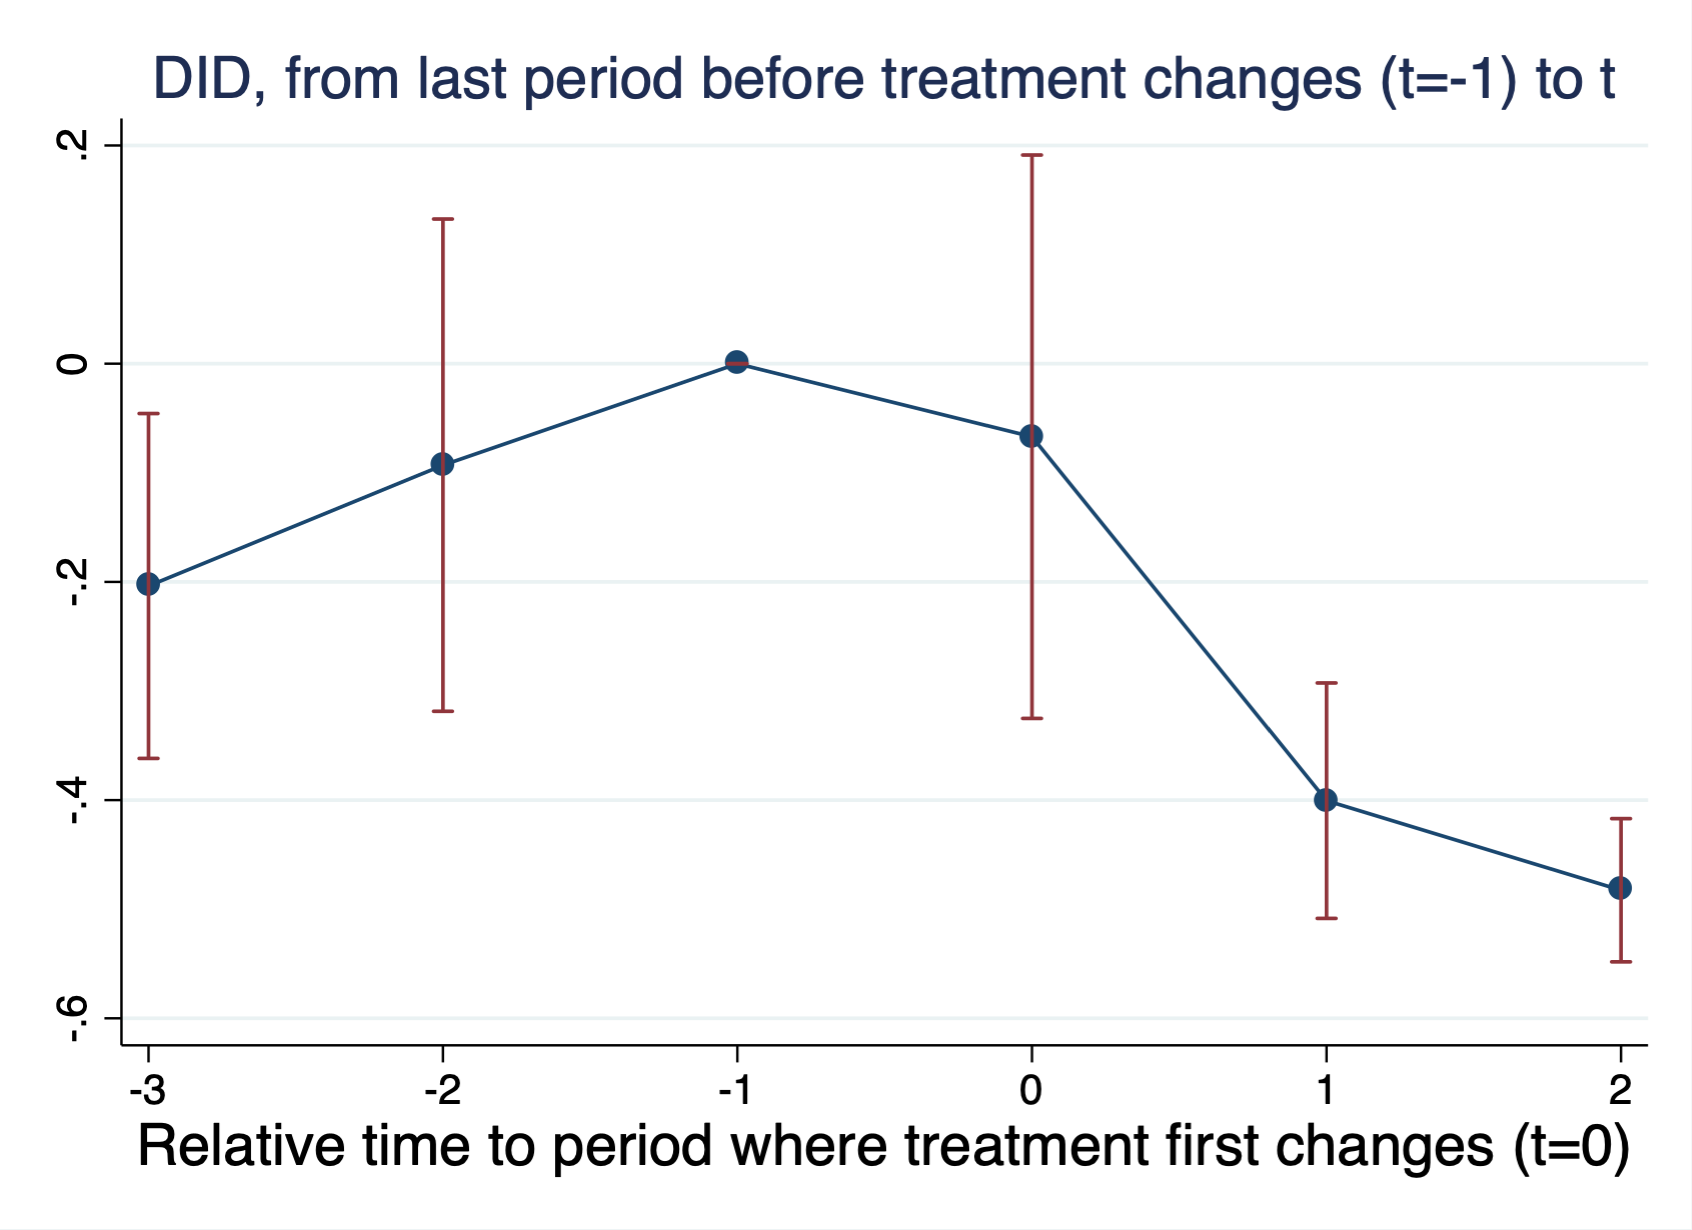
\includegraphics[width=1\textwidth]{Figures/chaisemartin_acuerdo.png}
       
 {\textbf Note: \citet{chaisemarting_etal_2019} two-way fixed effect model correction. The Figure shows 95\% confidence intervals, using 1,000 bootstrapped replications.} 
\end{figure} 

%Figure
\begin{figure}[h]  
\centering
\caption{Effect of Reelection Incentives on Centralization of Public Security (Sec. Agreement B)} 
\label{fig:chaisemartin_acuerdo2}

      
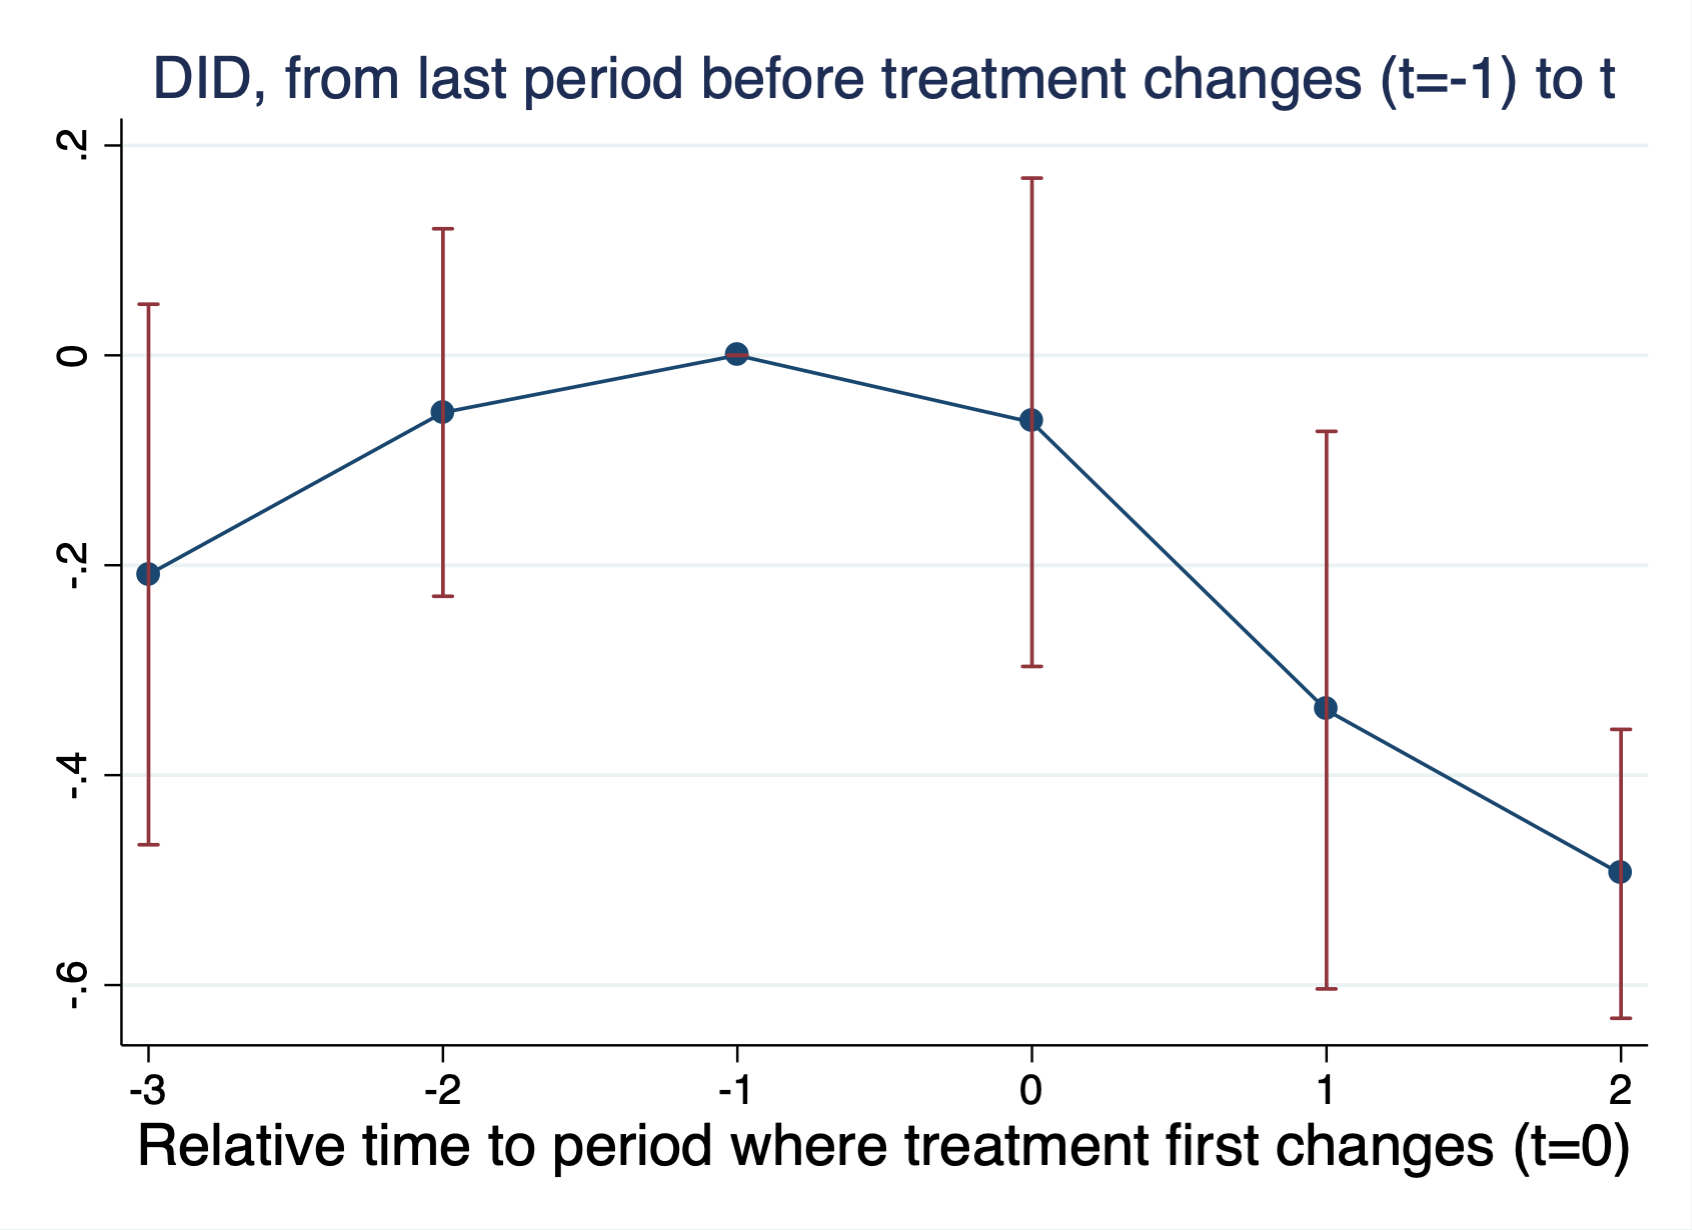
\includegraphics[width=1\textwidth]{Figures/chaisemartin_acuerdo2.png}
       
 {\textbf Note: \citet{chaisemarting_etal_2019} two-way fixed effect model correction. The Figure shows 95\% confidence intervals, using 1,000 bootstrapped replications.} 
\end{figure} 


%Figure
\begin{figure}[h]  
\centering
\caption{Effect of Reelection Incentives on Centralization of Public Security, Propensity Score Matching (Sec. Agreement A)} 
\label{fig:psm_acuerdo}

      
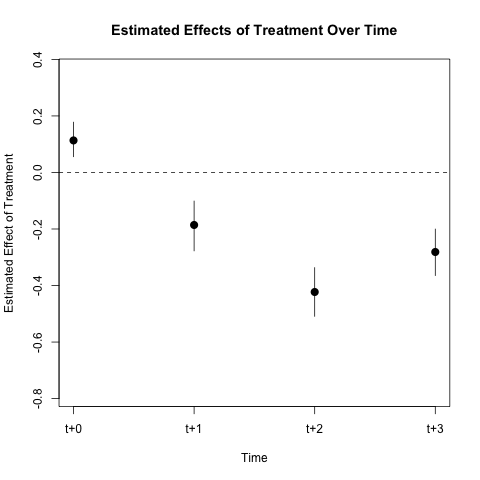
\includegraphics[width=1\textwidth]{Figures/mando_unico_psm.png}
       
 {\textbf Note: The Figure shows 95\% confidence intervals, using 1,000 bootstrapped replications.} 
\end{figure} 

%Figure
\begin{figure}[h]  
\centering
\caption{Effect of Reelection Incentives on Centralization of Public Security, Propensity Score Matching (Sec. Agreement B)} 
\label{fig:psm_acuerdo2}
   
      
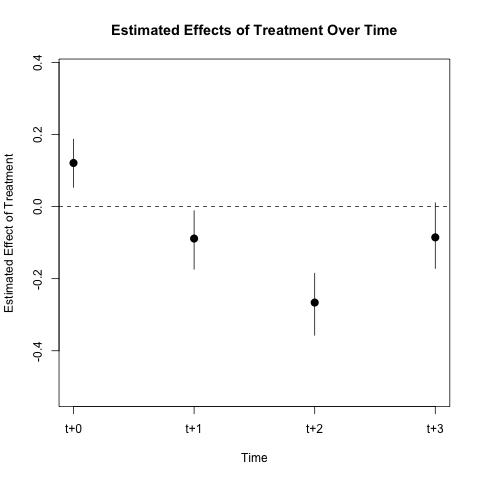
\includegraphics[width=1\textwidth]{Figures/mando_unico2_psm.png}
       
 {\textbf Note: The Figure shows 95\% confidence intervals, using 1,000 bootstrapped replications.} 
\end{figure} 

\clearpage
\subsection{Mechanism: Accountability}
 
 %Table
\begin{table}[htbp]\def\sym#1{\ifmmode^{#1}\else\(^{#1}\)\fi}
\centering
\caption{Effect of 2014 Term Limit Reform on Centralization, by security preferences}
\label{tab:chaisemartin_sec_preferences}
\scalebox{0.7}{
\begin{tabular}{lcccccccc}
\hline \hline
\\ \multicolumn{9}{l}{Dependent variable: Dummy signing Security Cooperaiton Agreement}\\
\addlinespace
& \multicolumn{2}{c}{Worried about Narco} & \multicolumn{2}{c}{Worried about insecurity} & \multicolumn{2}{c}{Worried about low punishment} & \multicolumn{2}{c}{Private expenses on home security}
& & \multicolumn{1}{c}{Below mean} & \multicolumn{1}{c}{Above mean} & \multicolumn{1}{c}{Below mean} & \multicolumn{1}{c}{Above mean} & \multicolumn{1}{c}{Below mean} & \multicolumn{1}{c}{Above mean} & \multicolumn{1}{c}{Below mean} & \multicolumn{1}{c}{Above mean} \\
& \multicolumn{1}{c}{(1)} & \multicolumn{1}{c}{(2)} & \multicolumn{1}{c}{(3)} & \multicolumn{1}{c}{(4)} & \multicolumn{1}{c}{(5)} & \multicolumn{1}{c}{(6)} & \multicolumn{1}{c}{(7)} & \multicolumn{1}{c}{(8)} \\
\cmidrule(lrr){2-3}  \cmidrule(lrr){4-5} \cmidrule(lrr){6-7} \cmidrule(lrr){8-9}  \\
\addlinespace
t-5 &        $ -0.052^{} $ &     $ -0.007^{} $ &     $ 0.000^{} $ &     $ -0.119^{} $ &    $ -0.001^{} $ &     $ 0.008^{} $ &     $ -0.052^{} $ &     $ -0.007^{} $ \\
& ($ 0.074$) & ($ 0.022 $) & ($ 0.000$) & ($ 0.082 $)  & ($ 0.001$) & ($ 0.016 $) & ($ 0.074$) & ($ 0.022 $) \\
t-4 &        $ -0.031^{} $ &     $ 0.052^{} $ &     $ 0.043^{} $ &     $ -0.038^{} $ &    $ -0.008^{} $ &     $ 0.038^{} $ &     $ -0.026^{} $ &     $ 0.063^{} $ \\
& ($ 0.024$) & ($ 0.068 $) & ($ 0.034$) & ($ 0.063 $)  & ($ 0.059$) & ($ 0.069 $) & ($ 0.023$) & ($ 0.066 $) \\
t-3 &        $ -0.007^{} $ &     $ 0.081^{} $ &     $ 0.007^{} $ &     $ 0.223^{} $ &    $ -0.004^{} $ &     $ 0.088^{} $ &     $ -0.000^{} $ &     $ 0.091^{} $ \\
& ($ 0.111$) & ($ 0.109 $) & ($ 0.035$) & ($ 0.174 $)  & ($ 0.022$) & ($ 0.129 $) & ($ 0.100$) & ($ 0.107 $) \\
t-2 &        $ 0.112^{} $ &     $ 0.141^{} $ &     $ 0.105^{} $ &     $ 0.064^{} $ &    $ 0.118^{***} $ &     $ 0.041^{} $ &     $ 0.136^{*} $ &     $ 0.091^{} $ \\
& ($ 0.128$) & ($ 0.199 $) & ($ 0.071$) & ($ 0.127 $)  & ($ 0.040$) & ($ 0.281 $) & ($ 0.076$) & ($ 0.185 $) \\
t=0 (Reform) &        $ 0.135^{} $ &     $ -0.185^{} $ &     $ 0.107^{***} $ &     $ -0.152^{} $ &    $ 0.071^{} $ &     $ -0.258^{} $ &     $ 0.145^{} $ &     $ -0.227^{} $ \\
& ($ 0.131$) & ($ 0.155 $) & ($ 0.034$) & ($ 0.135 $)  & ($ 0.127$) & ($ 0.199 $) & ($ 0.114$) & ($ 0.150 $) \\
t+1 &        $ 0.121^{} $ &     $ -0.689^{***} $ &     $ -0.159^{} $ &     $ -0.442^{**} $ &    $ -0.058^{} $ &     $ -0.732^{***} $ &     $ 0.050^{} $ &     $ -0.697^{***} $ \\
& ($ 0.121$) & ($ 0.115 $) & ($ 0.275$) & ($ 0.218 $)  & ($ 0.101$) & ($ 0.149 $) & ($ 0.135$) & ($ 0.118 $) \\
t+2 &        $ 0.109^{} $ &     $ -0.737^{***} $ &     $ -0.232^{} $ &     $ -0.402^{***} $ &    $ -0.220^{} $ &     $ -0.706^{} $ &     $ -0.022^{} $ &     $ -0.694^{***} $ \\
& ($ 0.242$) & ($ 0.096 $) & ($ 0.246$) & ($ 0.140 $)  & ($ 0.219$) & ($ 0.000 $) & ($ 0.298$) & ($ 0.122 $) \\
\addlinespace
Controls$^a$   &    \checkmark      &   \checkmark  &    \checkmark      &   \checkmark &    \checkmark      &   \checkmark &    \checkmark      &   \checkmark   \\
\hline \hline
\multicolumn{9}{p{1.5\textwidth}}{\footnotesize{Notes: Coefficients show corrected estimators following \citet{chaisemarting_etal_2019}. Standard errors in parentheses are clustered at the state level, with the following significance-level: $^{***}$ 1\%; $^{**}$ 5\%; and $^*$ 10\%.$^a$ Pre-treatment controls include the following: governor winning margin, mayor winning margin, governor and president party alignment dummies, and logged homicides per capita.}} \\
\end{tabular}
}
\end{table}

 

   
\clearpage


\subsection{Mechanism: Overgrazing} 

%\subsubsection{Bribes \& Corruption: Local police forces \& Military} 

 %Table
\begin{table}[H]\def\sym#1{\ifmmode^{#1}\else\(^{#1}\)\fi}
\centering
\caption{Bribes \& corruption: local police forces and the military level of effort}
\label{tab:reform_effort}
\scalebox{0.7}{
\begin{tabular}{lcccccccccc}
\hline \hline
    
            &\multicolumn{8}{c}{Sec. Coop. Agreement w/ Governor}                                                                                                                           \\\cmidrule(lr){2-9}
            &\multicolumn{1}{c}{(1)}         &\multicolumn{1}{c}{(2)}         &\multicolumn{1}{c}{(3)}         &\multicolumn{1}{c}{(4)}         &\multicolumn{1}{c}{(5)}         &\multicolumn{1}{c}{(6)}         &\multicolumn{1}{c}{(7)}         &\multicolumn{1}{c}{(8)}         \\
\addlinespace
t-7         &      0.0259         &      0.0984         &      0.5373         &     -0.1705\sym{**} &      0.0711         &     -0.0893         &      4.6488         &      0.1900         \\
            &    (0.2099)         &    (0.1082)         &    (0.5243)         &    (0.0814)         &    (0.0489)         &    (0.1095)         &    (4.9609)         &    (0.7083)         \\
\addlinespace
t-6         &      0.0845         &      0.1360         &     -0.0215         &     -0.0155         &     -0.2772         &     -0.0761         &     53.3145         &      1.6696\sym{**} \\
            &    (0.2927)         &    (0.1685)         &    (0.1761)         &    (0.1817)         &    (0.1989)         &    (0.0567)         &   (32.3619)         &    (0.7739)         \\
\addlinespace
t-5         &     -0.1601         &      0.1687         &     -0.0439         &     -0.3721\sym{**} &     -0.1118         &     -0.0960\sym{*}  &     17.1350\sym{*}  &      0.5027         \\
            &    (0.1914)         &    (0.1757)         &    (0.1561)         &    (0.1567)         &    (0.1257)         &    (0.0539)         &    (8.3739)         &    (0.6505)         \\
\addlinespace
t-4         &     -0.4814         &      0.0908         &     -0.0913         &     -0.5744\sym{***}&      0.0288         &     -0.0312         &     10.6996         &      0.0497         \\
            &    (0.2930)         &    (0.1378)         &    (0.1592)         &    (0.2065)         &    (0.0891)         &    (0.0309)         &    (8.4873)         &    (0.6807)         \\
\addlinespace
t-3         &     -0.2359         &      0.0429         &     -0.2455\sym{*}  &     -0.4114\sym{***}&     -0.2050         &     -0.0366         &     -4.9605         &     -1.0819         \\
            &    (0.3050)         &    (0.0748)         &    (0.1246)         &    (0.1383)         &    (0.1599)         &    (0.0401)         &    (8.1502)         &    (0.9116)         \\
\addlinespace
t-2         &     -0.1078         &     -0.0719         &     -0.2079         &     -0.3857\sym{**} &     -0.0472         &      0.0048         &      0.2610         &     -0.2297         \\
            &    (0.2224)         &    (0.0696)         &    (0.2195)         &    (0.1395)         &    (0.1694)         &    (0.0269)         &    (3.7753)         &    (0.5677)         \\
\addlinespace
Reform t=0  &      0.0272         &     -0.0567         &     -0.1501\sym{**} &     -0.0513         &     -0.0072         &     -0.0055         &      0.2961         &     -0.0721         \\
            &    (0.0622)         &    (0.0454)         &    (0.0633)         &    (0.0316)         &    (0.0147)         &    (0.0095)         &    (1.3202)         &    (0.2012)         \\
\addlinespace
t+1         &      0.0521         &     -0.0892         &     -0.2062\sym{***}&     -0.0529         &     -0.0151         &     -0.0246\sym{*}  &     -0.8786         &     -0.0030         \\
            &    (0.0985)         &    (0.0791)         &    (0.0669)         &    (0.0558)         &    (0.0392)         &    (0.0124)         &    (2.2503)         &    (0.3764)         \\
\addlinespace
t+2         &      0.0822         &     -0.1294         &     -0.2959\sym{***}&     -0.0562         &     -0.0907         &     -0.0472\sym{**} &     -0.6934         &      0.0301         \\
            &    (0.1521)         &    (0.1188)         &    (0.0930)         &    (0.0794)         &    (0.0554)         &    (0.0191)         &    (2.8772)         &    (0.5207)         \\
\addlinespace
t+3         &      0.0430         &     -0.1679         &     -0.3744\sym{***}&     -0.0466         &     -0.1088         &     -0.0698\sym{**} &      3.1119         &      0.2653         \\
            &    (0.1851)         &    (0.1595)         &    (0.1193)         &    (0.1016)         &    (0.0752)         &    (0.0253)         &    (2.9368)         &    (0.6721)         \\
\addlinespace
Observations&      14,587         &      14,587         &      14,587         &      14,587         &      14,587         &      14,587         &      14,587         &      14,587         \\
R2          &       0.839         &       0.337         &       0.359         &       0.366         &       0.856         &       0.603         &       0.655         &       0.640         \\
Controls    &  \checkmark         &  \checkmark         &  \checkmark         &  \checkmark         &  \checkmark         &  \checkmark         &  \checkmark         &  \checkmark         \\
Mun. FE     &  \checkmark         &  \checkmark         &  \checkmark         &  \checkmark         &  \checkmark         &  \checkmark         &  \checkmark         &  \checkmark         \\
Year FE     &  \checkmark         &  \checkmark         &  \checkmark         &  \checkmark         &  \checkmark         &  \checkmark         &  \checkmark         &  \checkmark         \\
State Cluster S.E.&  \checkmark         &  \checkmark         &  \checkmark         &  \checkmark         &  \checkmark         &  \checkmark         &  \checkmark         &  \checkmark         \\
Wild corr.  &                     &                     &                     &                     &                     &                     &                     &                     \\
Aggregate beta& $0.030^{}$$         &$-0.074^{}$$         &$-0.169^{***}$$         &$-0.030^{}$$         &$-0.041^{}$$         &$-0.027^{**}$$         & $0.613^{}$$         & $0.063^{}$$         \\
SE (aggregate)&       0.080         &       0.068         &       0.054         &       0.044         &       0.031         &       0.010         &       1.318         &       0.289         \\
p-value(aggregate)&       0.714         &       0.287         &       0.004         &       0.504         &       0.198         &       0.014         &       0.646         &       0.829         \\
 
                  
\hline \hline
\multicolumn{11}{p{1.5\textwidth}}{\footnotesize{Notes: Standard errors with the following significance-level: $^{***}$ 1\%; $^{**}$ 5\%; and $^*$ 10\%, that refer to two-sided test with the null hypothesis equal to 0.}} \\
\end{tabular}
} 
\end{table}

%Table
\begin{table}[htbp]\def\sym#1{\ifmmode^{#1}\else\(^{#1}\)\fi}
\centering
\caption{Effect of 2014 Term Limit Reform on effort of security forces}
\label{tab:chaisemartin_effort}
\scalebox{1}{
\begin{tabular}{lcc}
\hline \hline
\\ \multicolumn{3}{l}{Dependent variable:}\\
& \multicolumn{1}{c}{Local Police = log(detentions pc)} & \multicolumn{1}{c}{Military = log(laboratories errad.)$^{a}$} \\
& \multicolumn{1}{c}{(1)} & \multicolumn{1}{c}{(2)} \\
\cmidrule(lrr){2-2}  \cmidrule(lrr){3-3}\\
\addlinespace
Lag 3 years &        $ 0.011^{} $ &     $ -0.016^{} $ \\
& ($ 0.040$) & ($ 0.013 $) \\
Lag 2 years &        $ 0.057^{} $ &     $ -0.001^{} $ \\
& ($ 0.072$) & ($ 0.005 $) \\
Reform, time 0 &        $ -0.012^{} $ &     $ 0.006^{} $ \\
& ($ 0.039$) & ($ 0.006 $) \\
Lead 1 year &         $ -0.102^{***} $ &       $ -0.007^{**} $ \\
& ($ 0.036$) & ($ 0.003 $) \\
Lead 2 years &         $ -0.160^{} $ &      $ -0.012^{***} $  \\
& ($ 0.120$) & ($ 0.002 $) \\
\addlinespace
Controls$^b$   &    \checkmark      &   \checkmark    \\
\hline \hline
\multicolumn{3}{p{0.8\textwidth}}{\footnotesize{Notes: Coefficients show corrected estimators following \citet{chaisemarting_etal_2019}. Standard errors in parentheses are clustered at the state level, with the following significance-level: $^{***}$ 1\%; $^{**}$ 5\%; and $^*$ 10\%.$^a$ Secondary version of security cooperation agreements. $^b$ State-level controls include governor winning margin in last pre-treatment election and an indicator of whether the governor's party is the same as the federal incumbent party.}} \\
\end{tabular}
}
\end{table}


%Figure
\begin{figure}[h] 
\centering  
\caption{Effect of Term Limit Reform of 2014 on Security Forces Effort, IW estimators with 95\% confidence intervals \& SEs clustered state-level }
\label{fig:effort_security}
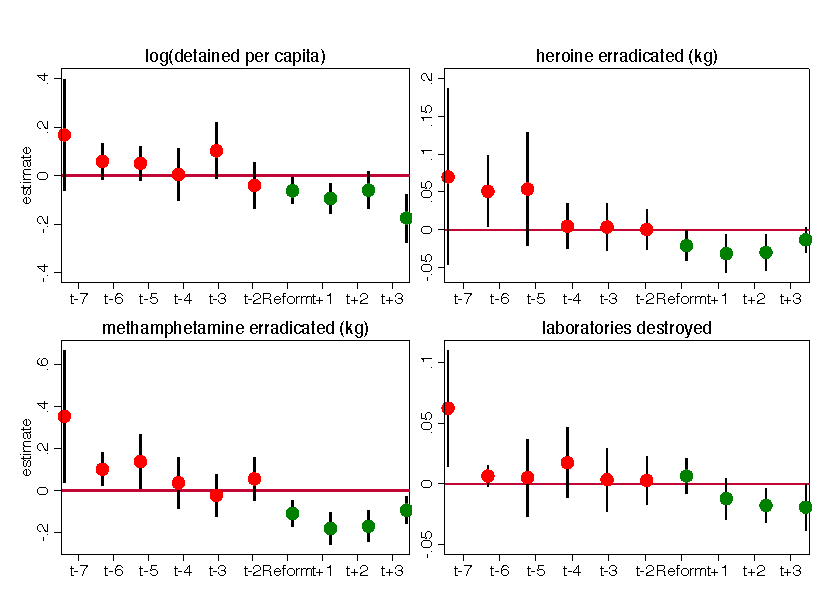
\includegraphics[width=0.65\textwidth]{Figures/effort_security.pdf}
       \captionsetup{justification=centering}

 {\footnotesize Note: IW estimators for each lead and lag relative to the first year of treatment.} 
    
 
 
\end{figure}  
       
\clearpage

    

%\subsubsection{Clientelistic Comparative Advantage: PRI vs. no PRI alignment} 
\bigskip

 %Table
\begin{table}[H]\def\sym#1{\ifmmode^{#1}\else\(^{#1}\)\fi}
\centering
\caption{Differential effect by Clientelistic Comparative Advantage}
\label{tab:alignment_pri}
\scalebox{0.7}{
\begin{tabular}{lccccccc}
\hline \hline
 
            &\multicolumn{3}{c}{DV: Agreement A}                              &\multicolumn{3}{c}{DV: Agreement B}                              \\\cmidrule(lr){2-4}\cmidrule(lr){5-7}
            &\multicolumn{1}{c}{(1)}         &\multicolumn{1}{c}{(2)}         &\multicolumn{1}{c}{(3)}         &\multicolumn{1}{c}{(4)}         &\multicolumn{1}{c}{(5)}         &\multicolumn{1}{c}{(6)}         \\
\addlinespace
Term Limit Reform&     -0.2942\sym{***}&     -0.2494\sym{***}&     -0.3477\sym{***}&     -0.2409\sym{***}&     -0.2007\sym{**} &     -0.3033\sym{***}\\
            &    (0.0716)         &    (0.0857)         &    (0.0692)         &    (0.0651)         &    (0.0786)         &    (0.0637)         \\
\addlinespace
Term Limit Reform (t-1)*Aligned (not PRI)&      0.1031         &                     &                     &      0.0458         &                     &                     \\
            &    (0.1406)         &                     &                     &    (0.1353)         &                     &                     \\
\addlinespace
Term Limit Reform (t-1)*Aligned (PRI)&                     &     -0.1253         &                     &                     &     -0.1210         &                     \\
            &                     &    (0.0917)         &                     &                     &    (0.0907)         &                     \\
\addlinespace
Term Limit Reform (t-1)*not aligned&                     &                     &      0.0929         &                     &                     &      0.1019         \\
            &                     &                     &    (0.0820)         &                     &                     &    (0.0813)         \\
\addlinespace
Observations&      14,761         &      14,761         &      14,761         &      15,652         &      15,652         &      15,652         \\
R2          &                     &                     &                     &                     &                     &                     \\
Controls    &  \checkmark         &  \checkmark         &  \checkmark         &  \checkmark         &  \checkmark         &  \checkmark         \\
Mun. FE     &  \checkmark         &  \checkmark         &  \checkmark         &  \checkmark         &  \checkmark         &  \checkmark         \\
Year FE     &  \checkmark         &  \checkmark         &  \checkmark         &  \checkmark         &  \checkmark         &  \checkmark         \\
Cluster S.E.&  \checkmark         &  \checkmark         &  \checkmark         &  \checkmark         &  \checkmark         &  \checkmark         \\
Tot.Int.    &     -0.1910         &     -0.3747         &     -0.2547         &     -0.1950         &     -0.3217         &     -0.2014         \\
S.E.(Tot. Int.)&      0.1511         &      0.0714         &      0.0871         &      0.1440         &      0.0679         &      0.0805         \\
p-value(Tot.Int.)&      0.2155         &      0.0000         &      0.0064         &      0.1853         &      0.0000         &      0.0178         \\
 
                  
\hline \hline
\multicolumn{7}{p{1.3\textwidth}}{\footnotesize{Notes: Standard errors with the following significance-level: $^{***}$ 1\%; $^{**}$ 5\%; and $^*$ 10\%, that refer to two-sided test with the null hypothesis equal to 0.}} \\
\end{tabular}
} 
\end{table}
   
%Table
\begin{table}[htbp]\def\sym#1{\ifmmode^{#1}\else\(^{#1}\)\fi}
\centering
\caption{Effect of 2014 Term Limit Reform on the likelihood of signing Security Cooperation Agreements}
\label{tab:chaisemartin_alignmentpri}
\scalebox{1}{
\begin{tabular}{lcc}
\hline \hline
\\ \multicolumn{3}{l}{Dependent variable:}\\
& \multicolumn{1}{c}{Alignment but not PRI} & \multicolumn{1}{c}{Alignment with PRI$^{a}$} \\
& \multicolumn{1}{c}{(1)} & \multicolumn{1}{c}{(2)} \\
\cmidrule(lrr){2-2}  \cmidrule(lrr){3-3}\\
\addlinespace
Lag 5 years &        $ -0.007^{} $ &     $ 0.000^{} $ \\
& ($ 0.008$) & ($ 0.000 $) \\
Lag 4 years &        $ -0.017^{} $ &     $ 0.068^{} $ \\
& ($ 0.044$) & ($ 0.052 $) \\
Lag 3 years &        $ 0.069^{} $ &     $ 0.044^{} $ \\
& ($ 0.112$) & ($ 0.055 $) \\
Lag 2 years &        $ 0.064^{} $ &     $ 0.118^{} $ \\
& ($ 0.181$) & ($ 0.097 $) \\
Reform, time 0 &        $ -0.028^{} $ &     $ -0.126^{} $ \\
& ($ 0.148$) & ($ 0.200 $) \\
Lead 1 year &         $ -0.315^{***} $ &       $ -0.505^{***} $ \\
& ($ 0.035$) & ($ 0.002 $) \\
Lead 2 years &         $ -0.426^{***} $ &      $ -0.510^{***} $  \\
& ($ 0.047$) & ($ 0.120 $) \\
\addlinespace
State Controls$^b$   &    \checkmark      &   \checkmark    \\
\hline \hline
\multicolumn{3}{p{0.6\textwidth}}{\footnotesize{Notes: Coefficients show corrected estimators following \citet{chaisemarting_etal_2019}. Standard errors in parentheses are clustered at the state level, with the following significance-level: $^{***}$ 1\%; $^{**}$ 5\%; and $^*$ 10\%.$^a$ Secondary version of security cooperation agreements. $^b$ State-level controls include governor winning margin in last pre-treatment election and an indicator of whether the governor's party is the same as the federal incumbent party.}} \\
\end{tabular}
}
\end{table}


%Table
\begin{table}[htbp]\def\sym#1{\ifmmode^{#1}\else\(^{#1}\)\fi}
\centering
\caption{Effect of 2014 Term Limit Reform on the likelihood of signing Security Cooperation Agreements}
\label{tab:chaisemartin_alignmentpri}
\scalebox{1}{
\begin{tabular}{lcc}
\hline \hline
\\ \multicolumn{3}{l}{Dependent variable:}\\
& \multicolumn{1}{c}{Alignment} & \multicolumn{1}{c}{Alignment with no PRI party$^{a}$} \\
& \multicolumn{1}{c}{(1)} & \multicolumn{1}{c}{(2)} \\
\cmidrule(lrr){2-2}  \cmidrule(lrr){3-3}\\
\addlinespace
Lag 5 years &        $ -0.011^{} $ &     $ -0.085^{} $ \\
& ($ 0.009$) & ($ 0.000 $) \\
Lag 4 years &        $ -0.003^{} $ &     $ 0.033^{} $ \\
& ($ 0.051$) & ($ 0.078 $) \\
Lag 3 years &        $ 0.056^{} $ &     $ 0.082^{} $ \\
& ($ 0.136$) & ($ 0.205 $) \\
Lag 2 years &        $ 0.113^{} $ &     $ -0.038^{} $ \\
& ($ 0.213$) & ($ 0.306 $) \\
Reform, time 0 &        $ -0.067^{} $ &     $ -0.049^{} $ \\
& ($ 0.156$) & ($ 0.259 $) \\
Lead 1 year &         $ -0.406^{***} $ &       $ -0.348^{**} $ \\
& ($ 0.049$) & ($ 0.173 $) \\
Lead 2 years &         $ -0.490^{***} $ &      $ -0.442^{} $  \\
& ($ 0.013$) & ($ 0.000 $) \\
\addlinespace
State Controls$^b$   &    \checkmark      &   \checkmark    \\
\hline \hline
\multicolumn{3}{p{0.6\textwidth}}{\footnotesize{Notes: Coefficients show corrected estimators following \citet{chaisemarting_etal_2019}. Standard errors in parentheses are clustered at the state level, with the following significance-level: $^{***}$ 1\%; $^{**}$ 5\%; and $^*$ 10\%.$^a$ Secondary version of security cooperation agreements. $^b$ State-level controls include governor winning margin in last pre-treatment election and an indicator of whether the governor's party is the same as the federal incumbent party.}} \\
\end{tabular}
}
\end{table}


 
\clearpage


\subsection{Mechanism: Capture}  

 %Table
\begin{table}[htbp]\def\sym#1{\ifmmode^{#1}\else\(^{#1}\)\fi}
\centering
\caption{Differential effect by Drug Cartel Presence}
\label{tab:centralization_homicides}
\scalebox{0.8}{
\begin{tabular}{lccccccc}
\hline \hline
 
            &\multicolumn{3}{c}{DV: Agreement A}                              &\multicolumn{3}{c}{DV: Agreement B}                              \\\cmidrule(lr){2-4}\cmidrule(lr){5-7}
            &\multicolumn{1}{c}{(1)}         &\multicolumn{1}{c}{(2)}         &\multicolumn{1}{c}{(3)}         &\multicolumn{1}{c}{(4)}         &\multicolumn{1}{c}{(5)}         &\multicolumn{1}{c}{(6)}         \\
\addlinespace
Term Limit Reform&     -0.1760         &      0.1786         &     -0.4620         &     -0.2245         &      0.0784         &     -0.4928         \\
            &    (0.4329)         &    (0.7543)         &    (0.5611)         &    (0.4524)         &    (0.8174)         &    (0.5881)         \\
\addlinespace
Term Limit Reform (t-2)*Worried about narcotraffick&      0.6773         &                     &                     &      1.1179         &                     &                     \\
            &    (2.1592)         &                     &                     &    (2.3462)         &                     &                     \\
\addlinespace
Term Limit Reform (t-2)*Worried about insecurity&                     &     -0.4750         &                     &                     &     -0.2727         &                     \\
            &                     &    (1.2076)         &                     &                     &    (1.3443)         &                     \\
\addlinespace
Term Limit Reform (t-2)*Punishment of criminals&                     &                     &      1.9447         &                     &                     &      2.1970         \\
            &                     &                     &    (2.7257)         &                     &                     &    (2.8906)         \\
\addlinespace
Observations&       7,572         &       9,097         &       9,097         &       7,909         &       9,530         &       9,530         \\
R2          &                     &                     &                     &                     &                     &                     \\
Controls    &  \checkmark         &  \checkmark         &  \checkmark         &  \checkmark         &  \checkmark         &  \checkmark         \\
Mun. FE     &  \checkmark         &  \checkmark         &  \checkmark         &  \checkmark         &  \checkmark         &  \checkmark         \\
Year FE     &  \checkmark         &  \checkmark         &  \checkmark         &  \checkmark         &  \checkmark         &  \checkmark         \\
Cluster S.E.&  \checkmark         &  \checkmark         &  \checkmark         &  \checkmark         &  \checkmark         &  \checkmark         \\
Tot.Int.    &      0.5013         &     -0.2964         &      1.4826         &      0.8934         &     -0.1943         &      1.7042         \\
S.E.(Tot. Int.)&      1.7460         &      0.4846         &      2.1881         &      1.9120         &      0.5523         &      2.3228         \\
p-value(Tot.Int.)&      0.7762         &      0.5459         &      0.5038         &      0.6441         &      0.7278         &      0.4695         \\
 
                  
\hline \hline
\multicolumn{7}{p{1.3\textwidth}}{\footnotesize{Notes: Standard errors with the following significance-level: $^{***}$ 1\%; $^{**}$ 5\%; and $^*$ 10\%, that refer to two-sided test with the null hypothesis equal to 0.}} \\
\end{tabular}
} 
\end{table}

%Table
\begin{table}[htbp]\def\sym#1{\ifmmode^{#1}\else\(^{#1}\)\fi}
\centering
\caption{Effect of 2014 Term Limit Reform on the likelihood of signing Security Cooperation Agreements}
\label{tab:chaisemartin}
\scalebox{1}{
\begin{tabular}{lcc}
\hline \hline
\\ \multicolumn{3}{l}{Dependent variable:}\\
& \multicolumn{1}{c}{No Cartel Presence} & \multicolumn{1}{c}{Cartel Presence$^{a}$} \\
& \multicolumn{1}{c}{(1)} & \multicolumn{1}{c}{(2)} \\
\cmidrule(lrr){2-2}  \cmidrule(lrr){3-3}\\
\addlinespace
Lag 5 years &        $ -0.050^{} $ &     $ -0.021^{} $ \\
& ($ 0.056$) & ($ 0.054 $) \\
Lag 4 years &        $ -0.007^{} $ &     $ 0.033^{} $ \\
& ($ 0.040$) & ($ 0.071 $) \\
Lag 3 years &        $ 0.050^{} $ &     $ 0.137^{} $ \\
& ($ 0.094$) & ($ 0.141 $) \\
Lag 2 years &        $ 0.097^{} $ &     $ 0.004^{} $ \\
& ($ 0.119$) & ($ 0.162 $) \\
Reform, time 0 &        $ -0.031^{} $ &     $ -0.170^{} $ \\
& ($ 0.112$) & ($ 0.153 $) \\
Lead 1 year &         $ -0.342^{***} $ &       $ -0.554^{**} $ \\
& ($ 0.082$) & ($ 0.266 $) \\
Lead 2 years &         $ -0.375^{***} $ &      $ -0.614^{***} $  \\
& ($ 0.086$) & ($ 0.174 $) \\
\addlinespace
State Controls$^b$   &    \checkmark      &   \checkmark    \\
\hline \hline
\multicolumn{3}{p{0.8\textwidth}}{\footnotesize{Notes: Coefficients show corrected estimators following \citet{chaisemarting_etal_2019}. Standard errors in parentheses are clustered at the state level, with the following significance-level: $^{***}$ 1\%; $^{**}$ 5\%; and $^*$ 10\%.$^a$ Secondary version of security cooperation agreements. $^b$ State-level controls include governor winning margin in last pre-treatment election and an indicator of whether the governor's party is the same as the federal incumbent party.}} \\
\end{tabular}
}
\end{table}

  
%Table 
\begin{table}[htbp]\def\sym#1{\ifmmode^{#1}\else\(^{#1}\)\fi}
\centering
\caption{Total Interaction Effect$^a$: the role of Alignment with the Party of the Governor and President}
\label{tab:abraham_sun_heteffects}
\scalebox{0.8}{
\begin{tabular}{lcccc}
\hline \hline
\\ \multicolumn{5}{l}{Dependent variable:}\\
& \multicolumn{2}{c}{acuerdo} & \multicolumn{2}{c}{acuerdo2$^{b}$} \\
& \multicolumn{1}{c}{(1)} & \multicolumn{1}{c}{(2)} & \multicolumn{1}{c}{(3)} & \multicolumn{1}{c}{(4)} \\
\cmidrule(lrr){2-3}  \cmidrule(lrr){4-5}\\
\addlinespace
Reform (t+3)*Dummy Cartel presence &     $ -0.4223^{**} $ &  &  $ -0.4594^{**} $  & \\
&     ($ 0.1705 $) &  & ($ 0.1893 $)  & \\
Reform (t+3)*Num. Carteles  &    &   $ -0.4088^{**} $ &  &  $ -0.5273^{**} $ \\
&    &     ($ 0.1671 $) & & ($ 0.2220 $)  \\
\\
\addlinespace
Observations       &             11,492    &             11,490    &          11,492      &           7,500  \\
R-squared       &        0.4599    &        0.4739    &     0.4599      &     0.4399  \\
Mun. FEs      &     \checkmark         &  \checkmark   &     \checkmark         &  \checkmark    \\
Year. FEs    &     \checkmark         &  \checkmark   &     \checkmark         &  \checkmark   \\
State Controls$^c$  &  \checkmark       &       \checkmark  &  \checkmark        &   \checkmark    \\
Cohort weighted$^d$  &   \checkmark      &       \checkmark  &   \checkmark       &   \checkmark    \\
\hline \hline
\multicolumn{5}{p{1\textwidth}}{\footnotesize{Notes:$^a$ Total interaction effect tests the linear hypothesis of the estimated coefficient of alignment with Federal Government indicator (winning margin) + estimated coefficient of the interaction of alignment (winning margin)*lead t=3. This is a post-estimation test using the same specification as that of Table \ref{tab:abraham_sun_lagdv} column (1). Other leads and the indicator at time t=0 when reform came to effect are omitted due to collinearity. Standard errors of linear hypothesis test in parentheses with the following significance-level: $^{***}$ 1\%; $^{**}$ 5\%; and $^*$ 10\%, that refer to two-sided test with the null hypothesis equal to 0. Main regression with standard errors clustered at the state-level. $^b$ Refers to the inverse hyperbolic sine transformation. $^c$ State-level controls include governor winning margin in last pre-treatment election and an indicator of whether the governor's party is the same as the federal incumbent party. I also include the lag of the outcome, i.e. logged homicides per capita as control. $^d$ Estimates weighted by each cohort's relative share of the sample following \citet{abraham_sun_2020}.}} \\
\end{tabular}
}
\end{table}

 
\clearpage 


\clearpage 


\end{appendix}
 
              

\begin{comment}
	 
\section{Potential sources of bias}

\begin{enumerate}
	\item Horizontal accountability institutions following \citet{weaver_2000}. 
	\item Information following Ethan bueno de mesquita paper. 
\end{enumerate}.  
\end{comment}

%Cites
%https://es.wikipedia.org/wiki/Anexo:Presidentes_municipales_de_Puebla_(2018-2021)
 
%http://www.snim.rami.gob.mx

%mechanisms: incumbency advantage, monitoring capacity of incumbent, 

\clearpage  
	


  
\end{document}
